\documentclass[sn-mathphys-num]{sn-jnl}%,authoryear

%\usepackage{apacite}


\usepackage{xcolor}
\newenvironment{mrevised}{\color{blue}}{}


\usepackage[utf8]{inputenc}


\usepackage{hyperref}
\hypersetup{
  linkcolor  = blue,
  citecolor  = blue,
  urlcolor   = blue,
  colorlinks = true,
}

\usepackage{soul}

%\usepackage{caption}
%\captionsetup[table]{skip=0.5pt}
\usepackage{graphicx}
\usepackage{amsmath}
\usepackage{amsthm}

\usepackage{latexsym}
\usepackage{amssymb}
\usepackage{amsfonts}
\usepackage[textwidth=0.65in,textsize=scriptsize]{todonotes}
\usepackage{proof}
\usepackage{verbatim}
\usepackage{url}
\usepackage{enumitem}
\usepackage{xspace}
\usepackage[draft]{fixme}
\usepackage[english]{babel}
\usepackage{stmaryrd}
\usepackage{upgreek}
\usepackage{cleveref}
\usepackage{booktabs}
%\usepackage{lineno}
%\usepackage[font=scriptsize,skip=0pt]{caption}
\usepackage[justification=centering]{caption}

% just for fixing font warnings
\usepackage{lmodern}
\usepackage{fix-cm}
\usepackage{stmaryrd}
\SetSymbolFont{stmry}{bold}{U}{stmry}{m}{n}

\usepackage{multicol}
\setlength{\multicolsep}{4pt plus 2pt minus 2pt}


% lists
\newlist{inlineenum}{enumerate*}{1}
\setlist[inlineenum,1]{label=\textbf{\textit{(\roman*)}}}

\newlist{compactitemize}{itemize}{1}
\setlist[compactitemize,1]{label=$\bullet$, leftmargin=1em, itemsep=0em}


% Environments
\theoremstyle{plain}
\newtheorem{theorem}{Theorem}
\newtheorem{proposition}[theorem]{Proposition}
\newtheorem{lemma}[theorem]{Lemma}
\newtheorem{corollary}[theorem]{Corollary}
\newtheorem{acknowledgements}[theorem]{Acknowledgements}
\newtheorem{claim}[theorem]{Claim}

\theoremstyle{definition}
\newtheorem{definition}[theorem]{Definition}
% \newtheorem{observation}[theorem]{Observation}

\theoremstyle{remark}
% \newtheorem{fact}[theorem]{Fact}
% \newtheorem{question}[theorem]{Question}
\newtheorem{example}[theorem]{Example}
%\newtheorem{remark}[theorem]{Remark}
% \newtheorem{sketch}[theorem]{Sketch}
% \newenvironment{nscenter}
%  {\parskip=2pt\par\nopagebreak\centering}
%  {\par\noindent\ignorespacesafterend}

\newenvironment{ctabular}[1]
{\begin{center}\begin{tabular}{#1}}
{\end{tabular} \end{center}}

\newenvironment{ltabular}[1]
{\begin{flushleft}\begin{tabular}{#1}}
{\end{tabular} \end{flushleft}}

\newenvironment{lttabular}[1]
{\begin{flushleft}\begin{tabular}[t]{#1}}
{\end{tabular} \end{flushleft}}

\newcommand{\nsparagraph}[1]{\noindent\textbf{#1}\,}
\newcommand{\ssparagraph}[1]{\bigskip\noindent\textbf{#1}\,}

\newcommand{\ti}[1]{\textit{#1}}
% \newcommand{\bs}[1]{\boldsymbol{#1}}
\newcommand{\ITM}[1]{{\bfseries \itshape (#1)}}

%Class of models
\newcommand{\classults}{\mathbf{M}}
\newcommand{\cultsfnu}{\mathbf{M}^{\mathbf{F}}_{\mathbf{NU}}}
\newcommand{\cultsfd}{\mathbf{M}_{\mathbf{FD}}}
\newcommand{\cultsnu}{\mathbf{M}_{\mathbf{NU}}}
\newcommand{\cultsac}{\mathbf{M}_{\mathbf{AC}}}
\newcommand{\cultsba}{\mathbf{M}_{\mathbf{BA}}}

\newcommand{\sults}{\mathbf{M}^1}

%Models
\newcommand{\modlts}{\mathcal{S}}
\newcommand{\modults}{\mathcal{M}}
\newcommand{\cmodel}{\modults^\Gamma}
\newcommand{\annsemantics}[2]{#1_{!#2}}
\newcommand{\annmodel}[1]{\modults_{!#1}}
\newcommand{\annmodelchi}{\annmodel{\chi}}
\newcommand{\arrowsemantics}[2]{#1_{{#2}}}
\newcommand{\arrowmodel}[1]{\modults_{{#1}}}
\newcommand{\arrowmodelU}{\arrowmodel{U}}

\newcommand{\clts}{\lts^\Gamma}
\newcommand{\D}[1]{\operatorname{D}_{#1}}
\newcommand{\DS}[1]{\operatorname{P}_{#1}}

\newcommand{\W}{\operatorname{W}}
\newcommand{\R}{\operatorname{R}}
\newcommand{\N}{\operatorname{N}}
\renewcommand{\S}{\operatorname{\asda}}
\newcommand{\Unc}{\operatorname{U}}
\newcommand{\Sother}{\operatorname{\mathbb{T}}}
\newcommand{\Ster}{\operatorname{\mathbb{U}}}
\newcommand{\V}{\operatorname{V}}
\newcommand{\compose}{{;}}
\newcommand{\REACH}[1]{(\leadsto_{#1}^*)}

\newcommand{\lts}{\textup{LTS}\xspace}
\newcommand{\ltss}{{\lts}s\xspace}
\newcommand{\ults}{\textup{LTS$^\text{\textup{U}}$}\xspace}
\newcommand{\ultss}{{\ults}s\xspace}

% Logical and proof symbols
\newcommand{\mldiam}[1]{\tup{#1}}
\newcommand{\mlbox}[1]{[#1]}
\newcommand{\kh}{{\sf Kh}}
\newcommand{\khi}{{\sf Kh}_i}
\newcommand{\lh}[2]{\tup{#1,#2}}
\newcommand{\blh}[2]{[#1,#2]}
\newcommand{\dialhepis}[1]{\tup{#1}}
\newcommand{\boxlhepis}[1]{[#1]}
\newcommand{\learn}{{\sf L}}
\newcommand{\arefdiam}{\tup{\not\sim}}
\newcommand{\arefbox}{[\not\sim]}
\newcommand{\gann}[1]{[!#1]}
\newcommand{\dgann}[1]{\tup{!#1}}
\newcommand{\refdiam}[2]{\tup{#1{\,\not\sim\,}#2}}
\newcommand{\refbox}[2]{[{#1{\,\not\sim\,}#2}]}
% \newcommand{\sarrowdiam}[2]{\tup{\tup{#1,#2}}}
% \newcommand{\sarrowbox}[2]{[\tup{#1,#2}]}
% \newcommand{\arrowdiam}[1]{\tup{#1}}
\newcommand{\arrowbox}[1]{[#1]}
\newcommand{\srefdiam}[1]{\tup{!#1}}
\newcommand{\srefbox}[1]{[!#1]}
\newcommand{\E}{{\sf E}}
\newcommand{\A}{{\sf A}}
\newcommand{\past}{\lozenge^{-1}}
\newcommand{\bpast}{\Box^{-1}}
\newcommand{\arbitrary}{{\mathsf{X}}}

\newcommand{\card}[1]{|{#1}|}
\newcommand{\subs}[1]{[#1]}
\newcommand{\natnum}{\mathbb{N}}
\newcommand{\intint}[2]{[#1 \mathop{...} #2]}

\newcommand\utimes{\mathbin{\ooalign{$\cup$\cr%
   \hfil\raise0.42ex\hbox{$\scriptscriptstyle\times$}\hfil\cr}}}
% \newcommand\utimes{\mathop{\ooalign{$\bigcup$\cr%
%    \hfil\raise0.36ex\hbox{$\scriptscriptstyle\boldsymbol{\times}$}\hfil\cr}}}

\newcommand{\PAL}{\textsf{PAL}\xspace}
\newcommand{\KHlogic}{\mathsf{L}_\kh}
\newcommand{\KHilogic}{\mathsf{L}_{\khi}}
\newcommand{\KHiMLlogic}{\mathsf{L}_{\khi,\square}}
\newcommand{\PAKHilogic}{\mathsf{PAL}_{\khi}}
\newcommand{\LHlogic}{\mathsf{L_{Lh}}}
\newcommand{\Reflogic}{\mathsf{L_{Ref}}}
\newcommand{\AReflogic}{\mathsf{L_{ARef}}}
\newcommand{\PlanReflogic}{\mathsf{L}_{\khi,\square,\srefbox{\plan}}}
\newcommand{\AtomReflogic}{\mathsf{L}_{\khi,\square,\srefbox{a}}}
\newcommand{\AgentReflogic}{\mathsf{L}_{\khi,\square,\srefbox{\plan,i}}}
% \newcommand{\SArrowlogic}{\mathsf{L_{SAU}}}
\newcommand{\AUL}{\mathsf{AUL}}
\newcommand{\AUKHilogic}{\AUL_{\khi}}
\newcommand{\KHaxiom}{\mathcal{L}_{\kh}}
\newcommand{\KHiaxiom}{\mathcal{L}_{\khi}\xspace}
\newcommand{\axset}{\mathcal{L}}
\newcommand{\axm}[1]{\textsf{#1}}

% completeness proof
\newcommand{\smcs}{\Upphi}
\newcommand{\restkh}[1]{#1\vert_{\kh}}
\newcommand{\restnkh}[1]{#1\vert_{\lnot\kh}}
\newcommand{\restkhi}[1]{#1\vert_{\khi}}
\newcommand{\restnkhi}[1]{#1\vert_{\lnot\khi}}
\newcommand{\resta}[1]{#1\vert_{\A}}
\newcommand{\restna}[1]{#1\vert_{\lnot\A}}
\newcommand{\restarbitrary}[1]{#1|_{\arbitrary}}
\newcommand{\restnarbitrary}[1]{#1|_{\lnot\arbitrary}}

% Tuples \tup{x,y} = <x,y>
\newcommand{\tup}[1]{\langle #1 \rangle}
% Tuples \ttup{x,y} = <<x,y>>
\newcommand{\ttup}[1]{\langle\!\langle \mathrm{#1} \rangle\!\rangle}

% Sets \set{x,y} = {x,y}
\newcommand{\set}[1]{\{ #1 \}}
% Sets with condition \setof{y}{xRy} = {y | xRy}
\newcommand{\setof}[2]{\{ #1  \mid #2 \}}

\newcommand{\ddiam}[1]{\ttup{#1}}
\newcommand{\pow}[1]{\mathcal P #1}
\newcommand{\setpaths}[1]{\mathcal P^{#1}}
\newcommand{\seqprop}{\bar{p}}
\newcommand{\seq}[1]{{\sf Seq}(#1)}
\newcommand{\lmodel}[3]{{#1}^{#2}_{#3}}

% Arrows
\renewcommand{\iff}{\mbox{\it iff}}
\newcommand{\siffs}{\;\iff\;}
\newcommand{\iffdef}{\ensuremath{\mbox{\it iff}_{\mbox{\tiny\it  def}}}}
\newcommand{\siffdefs}{\iffdef}
\newcommand{\ra}{\rightarrow}
\newcommand{\To}{\Rightarrow}
\newcommand{\lra}{\leftrightarrow}
\renewcommand{\implies}{\ra}
\newcommand{\inter}{\overset{int}{\longrightarrow}}
\newcommand{\rewtr}{\overset{\Tr}{\longrightarrow}}
\newcommand{\darrow}{\leftrightarrow}

% Definitions
\newcommand{\PROP}{{\rm \sf Prop}\xspace}
\newcommand{\FORM}{{\rm \sf Form}\xspace}
\newcommand{\AGT}{{\rm \sf Agt}\xspace}
\newcommand{\ACT}{{\rm \sf Act}\xspace}
\newcommand{\plans}{\uppi}
\newcommand{\plan}{\sigma}

% bisimulation
\newcommand{\bisim}{\xspace\mathrel{\raisebox{.5ex}{\small\ensuremath{\underline{\!\leftrightarrow\!}}}}\xspace}

% modal equivalence
\newcommand{\modequiv}{\leftrightsquigarrow}
\newcommand{\planequiv}{\mathrel{\leftrightarrows}}

% truth-set
\newcommand{\truthset}[2]{\llbracket #2 \rrbracket^{#1}}
\newcommand{\truthsetsyn}[2]{\mathopen{\{\!\vert} #2 \mathopen{\vert\!\}^{#1}}}

% format
\newcommand{\itm}[1]{{\bfseries \itshape (#1)}}



\newcommand{\exec}{\operatorname{E}}
\newcommand{\stexec}{\operatorname{SE}}


% arrows for executability
\newcommand{\ultsExec}{\Rightarrow}
\newcommand{\ultsExecStrat}[1]{\stackrel{#1}{\ultsExec}}
\newcommand{\ultsExecAgi}{\stackrel{i}{\ultsExec}}


\newcommand{\learnset}[3]{\operatorname{learn}(#1, #2, #3)}
\newcommand{\splitstr}[4]{#1 \leadsto^{#3}_{#4} #2}


%Partition
% To write notes in the text
\newcommand{\raul}[1]{\todo[color=red!30]{{\bf Raul:} {\footnotesize #1}}\xspace}
\newcommand{\bigraul}[1]{\todo[inline,color=red!30]{{\bf Raul:} {\footnotesize #1}}}

\newcommand{\fer}[1]{\todo[color=blue!20]{{\bf Fer:} {\footnotesize #1}}\xspace}
\newcommand{\bigfer}[1]{\todo[inline,color=blue!20]{{\bf Fer:} {\footnotesize #1}}}

\newcommand{\carlos}[1]{\todo[color=green!20]{{\bf Carlos:} {\footnotesize #1}}\xspace}
\newcommand{\bigcarlos}[1]{\todo[inline,color=green!20]{{\bf Carlos:} {\footnotesize #1}}}

\newcommand{\andres}[1]{\todo[color=cyan!20]{{\bf ARS:} {\footnotesize #1}}\xspace}
\newcommand{\bigandres}[1]{\todo[inline,color=cyan!20]{{\bf ARS:} {\footnotesize #1}}}

\newenvironment{comfer}
{ \color{blue} }
{ \normalcolor }


\newenvironment{comraul}
{ \color{red} }
{ \normalcolor }

\newcommand{\colornuevo}{orange}
\newcommand{\nuevo}[1]{\textcolor{\colornuevo}{#1}}

\newenvironment{textonuevo}
{\color{\colornuevo}}
{\normalcolor}

\newcommand{\hlight}[1]{{\setlength{\fboxsep}{2pt}\colorbox{yellow!75!red}{#1}}}
%{\sethlcolor{yellow!25!red}\hl{#1}}

\newcommand{\nota}[1]{\textcolor{red}{#1}}
\newcommand{\notabis}[1]{\textcolor{blue}{#1}}


%Abbreviated Cref
\Crefname{definition}{Def.}{Defs.}
\Crefname{equation}{Eq.}{Eqs.}
\Crefname{figure}{Fig.}{Figs.}
\Crefname{proposition}{Prop.}{Props.}
\Crefname{theorem}{Thm.}{Thms.}
\Crefname{example}{Ex.}{Exs.}
\Crefname{corollary}{Cor.}{Cors.}
\Crefname{inlineenumi}{Item}{Items}
\Crefname{enumi}{Item}{Items}
\Crefname{section}{Sec.}{Secs.}
\Crefname{appendix}{App.}{Apps.}

\newcommand{\Crefitem}[1]{\Cref{#1}}



\usepackage{tikz}
%\usetikzlibrary{automata,arrows,backgrounds,positioning,fit,calc,matrix,decorations.pathmorphing}
\usetikzlibrary{arrows,decorations,shapes,automata,positioning,decorations.pathmorphing}

\tikzset{
  every picture/.style = {
    thick,
    >=stealth',
    node distance = 1.5em and 3em,
  }
  ,
  cross line/.style = {
    preaction = {
      draw=white,
      -,
      line width=4pt
    }
  }
  ,
  state/.style = {
    rectangle,
    rounded corners = 5pt,
    font = \footnotesize,
    draw,
    minimum width = 1em,
    minimum height = 1em
  }
  , % labels of states
  label-state/.style = {
    sloped,
    font = \scriptsize,
    label distance = -2pt
  }
  , % labels of edges
  label-edge/.style = {
    font = \scriptsize,    
    label distance = -2pt
  }
}

% Complexity
\newcommand{\NP}{{\rm\textsf{NP}}\xspace}
\newcommand{\Poly}{{\rm\textsf{P}}\xspace}
\newcommand{\PSPACE}{{\rm\textsf{PSpace}}\xspace}
\newcommand{\EXPSPACE}{{\rm\textsf{ExpSpace}}\xspace}
\newcommand {\EXPTIME} {\rm\textsf{ExpTime}\xspace}
\newcommand {\NEXPTIME} {\rm\textsf{NExpTime}\xspace}
\newcommand{\PH}{{\rm\textsf{PH}}\xspace}



\begin{document}

\title[The Dynamics of Knowing How]{The Dynamics of Knowing How}

\author*[1,2]{\fnm{Carlos} \sur{Areces}}\email{carlos.areces@unc.edu.ar}
\author*[1,2]{\fnm{Raul} \sur{Fervari}}\email{rfervari@unc.edu.ar}
\author*[1,2]{\fnm{Andr\'es R.} \sur{Saravia}}\email{andresrsaravia@mi.unc.edu.ar}
\author*[3]{\fnm{Fernando R.} \sur{Vel\'azquez-Quesada}}\email{fernando.velazquezquesada@uib.no}

\affil[1]{\orgname{Consejo Nacional de Investigaciones Científicas y Técnicas ({CONICET})}, \country{Argentina}}
% \orgdiv{Department}, 
% \orgaddress{\street{Godoy Cruz}, \city{Ciudad Autónoma de Buenos Aires}, \postcode{C1425FQB}, \state{CABA}}

\affil[2]{\orgname{Universidad Nacional de Córdoba (UNC)}, \orgaddress{\state{Córdoba}, \country{Argentina}}}
% \orgaddress{\street{Av. Medina Allende}, \city{Córdoba}, \postcode{X5000HUA}, \state{Córdoba}, 

\affil[3]{\orgname{Universitetet i Bergen}, \orgaddress{\state{Bergen}, \country{Norway}}}

%\linenumbers

\abstract{
We investigate dynamic operations acting over a knowing how logic. Our approach uses a recently introduced semantics for the knowing how operator, based on an indistinguishability relation between plans, and arguably closer to the standard presentation of knowing that modalities in classic epistemic logic. 
Here, we discuss how the new indistinguishability-based semantics enables us to define dynamic modalities representing different ways in which an agent can learn how to achieve a goal. In this regard, we study different alternatives for implementing two types of updates: ontic and epistemic.
For the former, we provide axiomatizations over a restricted class of models. For the latter, we investigate some semantic properties and discuss what are the difficulties in axiomatizing dynamic modalities. In turn, we introduce a novel dynamic epistemic modality for which we have reduction axioms, over an extended static language of knowing how.
}

\keywords{Knowing how, updates, axiomatization, decidability}

\maketitle

%\newpage
%\tableofcontents

\section{Introduction}
\label{sec:intro}
%\begin{textonuevo}
% #4.1: knowing that + its dynamics + how those ideas can be used for knowing how (KH)
The notion of \emph{knowing that} has been one of the fundamental study subjects in Epistemology. It concerns the knowledge an agent might have about the truth-value of propositions, and as such has driven most of the field's research agenda, with some authors even claiming that it subsumes many other forms of knowledge~(see, e.g., \cite{BoenLycan75,stanley2001knowing,Snowdon2004}). 

 
One of the most successful tools for studying this concept has been Epistemic Logic (EL; \cite{Hintikka:kab}), a formal logical framework which, on the semantic side, typically relies on pointed Kripke models~\cite{mlbook,HML}. In more detail, a Kripke model is a relational structure whose domain's elements (called possible states/situations/worlds) represent the different ways the real world can be, and in which a binary \emph{epistemic indistinguishability} relation represents the agent's uncertainty. Then, a pointed Kripke model is a Kripke model with a distinguished evaluation state, usually understood as describing the actual situation. With this, knowledge about the truth-value of propositions is defined as follows: at a given state $w$, the agent knows that a proposition $\varphi$ is true if and only if $\varphi$ holds in all the states she cannot distinguish from $w$. Asking for the indistinguishability relation to be reflexive, transitive and Euclidean (i.e., an equivalence relation) makes knowledge truthful, positively and negatively introspective. EL has proved to be a useful tool for developments in, e.g., Philosophy~\cite{rfe,Holliday2018}, Computer Science~\cite{RAK}, AI~\cite{elfaics} and Economics~\cite{egepgt}. In achieving this, one of its most appealing aspects is that it can be used to reason about information change. Indeed, actions that increase the agent's knowledge can be straightforwardly represented as model operations that remove edges, thus reducing the agent's uncertainty. Further research on this idea has given rise to Dynamic Epistemic Logic (DEL), a field that studies how the attitudes of a set of agents change through diverse informational actions (see, e.g.,~\cite{DELbook,vanBenthem2011ldii}). 

%\smallskip

% #1: motivating KH
Still, knowing that is not the only form of knowledge an agent might have/use. In fact, the last few years have witnessed the emergence of formal frameworks for reasoning about knowing whether, knowing how, knowing why, knowing what, and so on (see~\cite{Wang16} for an overview). Among them, knowing how (e.g.,~\cite{Pavese22}) is one of the most important, as it concerns the knowledge an agent has about her \emph{ability} to achieve a given outcome. Intuitively, an agent knows how to achieve~$\varphi$ given~$\psi$ if she has at her disposal a suitable \emph{course of action} guaranteeing that $\varphi$ will be the case whenever she is in a situation in which $\psi$ holds. It is worthwhile to study  this notion not only from a philosophical perspective, but also from a computer science point of view, as the concept can be seen, for example, as a formal account for automated planning and strategic reasoning in AI (see, e.g.,~\cite{KandA15}).

% #2: knowing that (KT) + ability is not enough, and a brief description of LTS semantics
Most traditional approaches for representing knowing how rely on combining logics of knowing that with logics of action (see, e.g.,~\cite{Mccarthy69,Les00,HerzigT06}). However, while a combination of operators for knowing that and \emph{ability} (e.g.,~\cite{wiebeetal:2003}) produces a \emph{de dicto} reading of the concept (\emph{``the agent knows she has an action that guarantees the goal''}), a proper notion of \emph{``knowing how to achieve $\varphi$''} requires a \emph{de re} clause (\emph{``the agent has an action that she knows guarantees the goal''}; see~\cite{JamrogaA07,Herzig15} for a discussion). Based on these considerations, \cite{Wang15lori,Wang2016} introduced a framework based on a knowing how binary modality $\kh(\psi,\varphi)$. At the semantic level, this language is also interpreted over relational models --- called labeled transition systems (LTSs) in this context. The difference with respect to the EL setting is that, here, relations describe the actions an agent considers she has at her disposal (in some sense, her \emph{epistemic abilities}).
%An edge labeled $a$ going from state $w$ to state $u$ indicates that the agent can execute action $a$ to go from $w$ to $u$. Thus,
Then, $\kh(\psi,\varphi)$ holds if and only if there is a ``proper plan'' (a sequence of actions satisfying certain constraints) in the LTS that unerringly leads from every $\psi$-state only to $\varphi$-states.


% #3: introducing indistinguishability and discussing its benefits
While variants of this idea have been explored in the literature (see, e.g.,~\cite{Li17,LiWang17,FervariHLW17,Wang19a,LiW24}),
%weakens the contraints on the required plan, \cite{LiWang17} adds requirements on the plan's intermediate states, \cite{FervariHLW17} combines it with a \emph{knowing that} operator.}
most of them share the fundamental feature mentioned above: relations in the model are interpreted as the agent epistemic take on her available actions. Due to this, the epistemic abilities of an agent depend \emph{only} on what these actions can achieve. The framework presented in~\cite{AFSVQ21,AFSVQ23report} changed this by adding a notion of indistinguishability between plans, related to the notion of \emph{strategy indistinguishability} (e.g.,~\cite{JamrogaH04,Belardinelli14}). Two main insights are introduced in these articles. The first is simple: while certain plans might be available in a given environment, they might not be available \emph{to a given agent} (e.g., she might not know about them, or did not consider them at the given time). Hence, not all possible plans are available to all agents.  More importantly, she might consider some of these plans \emph{indistinguishable} from some others\footnote{The exact meaning of ``indistinguishable'' is left open. In particular, it does not necessarily mean that the agent cannot tell the plans apart, it might just be that she considers the differences not relevant.}. In such cases, having available a proper plan $\plan$ that leads from any $\psi$-state to only $\varphi$-states is not enough: the agent also needs for \emph{all the plans she cannot distinguish from $\plan$} to satisfy the same requirement. 
As argued in~\cite{AFSVQ21}, the benefits of these new semantics are threefold. First, it provides an indistinguishability-based view of an agent's epistemic abilities, akin to the EL approach for modeling knowing that. Second, it can deal with multi-agent scenarios more naturally. Third, it leads to a natural definition of operators representing dynamic aspects of knowing how, akin to the DEL approach for modeling dynamics of knowing that.
%
% This is in sharp contrast with standard epistemic logic (EL)~\cite{Hintikka:kab}, where relational models have two kinds of information: ontic facts about a given situation (represented by the current state in the model), and the particular perspective that agents have (represented by the possible states available in the model, and their respective indistinguishability relation between them). If one would like to mirror the situation of EL, it seems natural that \emph{knowing how} should be defined in terms of some kind of indistinguishability over the  information provided by an LTS.  Such an extended model would be able to capture both the abilities of an agent as given by her available actions, together with the (in)abilities that arise when considering two different actions/plans/executions indistinguishable.
%
%Syntactically, its main component is a binary modality $\khi(\psi,\varphi)$, for each agent~$i$.  Semantically, the crucial idea is the inclusion of an indistinguishability relation between plans over an \lts for each agent $i$, on top of the \lts.
%
%The new structures are called \emph{uncertainty-based \lts} (\ults). Then, formulas are interpreted over \ultss. In this proposal, an agent may have different alternatives at her disposal to try to achieve a goal, all ``as good as any other'' (and in that sense indistinguishable) as far as she can tell. In this way, \ultss aim to reintroduce the notion of epistemic indistinguishability, now at the level of plans.
%
%\end{textonuevo}

%\smallskip


This article focuses on the latter point, using this in\-dis\-tin\-guisha\-bil\-i\-ty-based semantics to study several dynamic operators describing changes in the agents' epistemic abilities. To the best of our knowledge, this is the first time this theme is addressed (except by the brief discussion in~\cite{Wang2016} about knowing how and announcements, and the work in~\cite{AFSV22} that this article extends). The proposals follow the DEL approach, using changes in the model to represent changes in the situation they describe. In doing so, we take advantage of the fact that, in these structures, there is a clear distinction between ontic and epistemic information. Indeed, while the underlying LTS contains \emph{ontic} facts common to all agents (the available actions as well as their effect), the indistinguishability relation over plans represents the \emph{epistemic} perception of each particular agent (the plans an agent considers available, as well as her capacity to distinguish between thems). Thus, model-update operations affecting different parts of the model have a clear-cut interpretation: while changes in the LTS can be seen as ontic updates (with possible epistemic consequences), changes in plan indistinguishability relation can be seen as direct epistemic ones. 

%-----------------------
% The previous text

%\fer{Still to revise from here to the end of the intro}The paper starts by investigating operators that update models based on some sort of \emph{announcement}, in the spirit of~\cite{Plaza89:lopc}. By following closely standard definitions of announcements, the operation results in an ontic update in our setting. This is because accessibility relations and states in the LTS represent objective information available for the agents. Then, we will define operations that perform epistemic updates. In particular, we will discuss ways in which the indistinguishability relation between plans can be refined, causing some change in the agents' knowledge. With these proposals, we illustrate the difficulties of dealing with this kind of modalities in the context of knowing how logics. More precisely, we will present the main challenges that arise in axiomatizing these new dynamic modalities. We discuss both how the failure of the uniform substitution property in the logics, and the weak expressive power of the base static logic are obstacles in defining a complete axiomatization for some dynamic modalities. As a consequence, as a novelty with respect to~\cite{AFSV22}, we introduce a new proposal, in which we extend the underlying (static) knowing how logic, with basic modalities $\mlbox{a}$, for each action $a$, and with a dynamic modality $\srefbox{\plan}$, revealing the possibility of executing $\plan$, and differentiating it from the rest of the available plans. With this additional expressivity, we can obtain a completeness result for the resulting dynamic logic, via reduction axioms.

%\smallskip

%\noindent\textbf{Outline:} This article is organized as follows. \Cref{sec:basic} recalls the basic definitions of the indistinguishability-based knowing how setting (\cite{AFSVQ21,AFSVQ23report}), including results that are useful in the rest of this manuscript.  Interestingly, we show that one of the axioms presented in~\cite{AFSVQ21,AFSVQ23report} can be removed as it is derivable from the others. In~\Cref{sec:ontic} ontic updates are investigated, based on public announcements~\cite{Plaza89:lopc} and arrow updates~\cite{KooiR11}. We discuss the properties of the operations, and provide reduction axioms over a very restricted class of models. In~\Cref{sec:epistemic-basic} we provide alternatives for epistemic updates, and discuss some of their semantic properties. In particular, we prove that uniform substitution does not hold in general. \Cref{sec:extension} introduces a new proposal in which epistemic updates are defined over an extended language, and provides a complete axiomatization via reduction axioms. Moreover, we show that the satisfiability problem for the resulting logics is decidable, using filtrations. Finally, in~\Cref{sec:final} we offer some final remarks and discuss future lines of work.

%-----------------------
% an initial attempt

%The paper starts by investigating \emph{ontic} change, and the focus is two-fold: first, an operation removing states (in the spirit of~\cite{Plaza89:lopc}), and then one removing edges (in the spirit of~\cite{KooiR11}). Still, the main focus is \emph{epistemic} change. In the initial phase, the focus is two-fold too: first, an operation eliminating uncertainty between specific plans, and then one that quantifies over the former by quantifying over plan refinement. 

%The modalities used for describing the effects of all these operations increase the expressivity of the basic language, and thus an axiomatisation via reduction axioms is not possible. In the case of ontic updates, this leads to an alternative strategy: restrict the setting to a particular class of models. In the case of epistemic updates, this leads to a second phase in which the basic language is extended with a standard modality for each basic action. In this new setting, a further model-update operation is studied, for which a reduction-axiom-based axiomatisation is provided.

%\smallskip

%\noindent\textbf{Outline:} This article is organized as follows. \Cref{sec:basic} recalls the basic definitions of the indistinguishability-based \emph{knowing how} setting, including results that are useful in the rest of this manuscript. (Interestingly, we show that one of the axioms is derivable from the others.) \Cref{sec:ontic} investigates ontic updates via (variations of) well-known state-removing and edge-removing operations, then providing reduction axioms over a restricted class of models. \Cref{sec:epistemic-basic} is the initial exploration of alternatives for epistemic updates, and \Cref{sec:extension} extends the basic setting to introduce a new proposal in which epistemic updates are defined over an extended language. \Cref{sec:final} closes by offering some final remarks and discussing future lines of work.

%-----------------------
% new version

\medskip

\begin{mrevised}
The rest of the article is organized in the following way. \Cref{sec:basic} recalls the basic definitions of the indistinguishability-based knowing how setting \cite{AFSVQ21,AFSVQ23report}, including some new results. In particular, we show that one of the axioms presented in the axiomatization introduced in \cite{AFSVQ21,AFSVQ23report} is derivable from the others, while a new axiom is needed to fix a small gap in the completeness argument. We also discuss some results concerning the expressive power of the basic knowing how logic over particular classes of models. 

\Cref{sec:ontic,sec:epistemic-basic,sec:extension} constitute the core of the contribution. Indeed, \Cref{sec:ontic}, investigates \emph{ontic} updates by introducing model operations that affect the ontic components of the models: first an operation that removes states (in the spirit of~\cite{Plaza89:lopc}) and then one that removes edges (in the spirit of~\cite{KooiR11}). Then, \Cref{sec:epistemic-basic,sec:extension} are devoted to \emph{epistemic} updates. While \Cref{sec:epistemic-basic} discusses two operations for eliminating uncertainty between plans (the first works over two given plans; the second quantifies over the parameters of the first),\footnote{The dynamic operators associated with these updates were first introduced in~\cite{AFSV22}. Here we provide a more detailed analysis and complete proofs.} \Cref{sec:extension}
introduces an epistemic update that makes a given plan distinguishable from any other. \Cref{sec:final} closes the article by offering some final remarks and discussing future lines of work.

Among the results presented in \Cref{sec:ontic,sec:epistemic-basic,sec:extension}, one can highlight the following. First, it is  shown that the modalities capturing the model updates from \Cref{sec:ontic,sec:epistemic-basic} lead to an increase of the expressive power of the resulting logic, w.r.t.\ the classical knowing how logic. Hence, an axiomatization via reduction axioms is not possible. For the ontic updates, reduction axioms can be defined when we restrict the logic to a particular class of models, but this approach does not work for the epistemic modalities. The modality associated to the update of \Cref{sec:extension} also increases the expressive power, and hence no reduction axioms exist. However, reduction axioms can be obtained by further extending the language with standard modalities for each basic action. 
 
\end{mrevised}


\section{Preliminaries}
\label{sec:basic}
%\nsparagraph{Syntax and semantics.}
This section recalls the syntax and semantics of the knowing how framework as presented in~\cite{AFSVQ21} as well as a complete axiomatization and a suitable notion of bisimulation (both from~\cite{AFSVQ23report}). It also discusses some complexity and expressivity results. Throughout the text, let $\PROP$ be a countable set of propositional symbols, $\ACT$ a denumerable set of action symbols, and $\AGT$ a non-empty finite set of agents.

\medskip

\begin{definition}\label{def:khsyntax}
Formulas of the language $\KHilogic$ are defined by the following grammar:
\begin{spcenter}
  $\varphi ::= p \mid \neg\varphi \mid \varphi\vee\varphi \mid \khi(\varphi,\varphi)$,
\end{spcenter}
with $p \in \PROP$ and $i\in\AGT$. Other Boolean connectives are defined as usual. Formulas as $\khi(\psi,\varphi)$ state that \emph{``when $\psi$ is the case, agent $i$ knows how to make $\varphi$ true''}. Define also the abbreviations $\A\varphi:=\khi(\neg\varphi,\bot)$ for an arbitrary $i$, and $\E\varphi:=\neg\A\neg\varphi$.
% as established in~\cite{AFSVQ21}, they behave exactly as the universal and existential modalities (see, e.g.~\cite{GorankoP92}), respectively.
\end{definition}
\medskip

In~\cite{Wang15lori,Wang2016}, formulas are interpreted
over \emph{labeled transition systems} (\ltss): relational
models in which each (basic) relation indicates the source and target
of a particular type of action the agent can perform.
In the setting introduced in~\cite{AFSVQ21}, \lts{s} are extended with a notion of \emph{uncertainty} between plans.

% \begin{definition}[Labeled Transition Systems]\label{def:abmap}
%   A \emph{labeled transition system (LTS)} is a tuple
%   $\modlts=\tup{\W,\R,\V}$ where $\W$ is a non-empty set of states (called the domain and
%   denoted by $\D{\lts}$),
%   $\R = \setof{\R_a \subseteq \W \times \W}{a \in \ACT}$ is a
%   collection of binary relations on $\W$, and $\V:\W \to 2^\PROP$ is a
%   labeling function. For $w\in\W$, the pair $(\modlts,w)$ is a
%   \emph{pointed LTS}, with parentheses usually dropped.
% \end{definition}
\medskip

\begin{definition}[Actions and plans]
Let $\ACT^*$ be the set of finite sequences over $\ACT$. Elements of
$\ACT^*$ are called \emph{plans}, with $\epsilon$ being the
\emph{empty plan}. %Let $\ACT^+ := \ACT^* \setminus  \set{\epsilon}$.
Given $\plan \in \ACT^*$, we use $\card{\plan}$ to denote its length (in particular, $\card{\epsilon} = 0$). For
$0 \le k \le \card{\plan}$, the plan $\plan_k$ is $\plan$'s initial
segment up to (and including) the $k$th position (with
$\plan_0 := \epsilon$). For $0 < k \le \card{\plan}$, the action
$\plan[k]$ is the one in $\plan$'s $k$th position.
\end{definition}

\medskip

\begin{definition}[Uncertainty-based \lts]\label{def:ults}
%Let \AGT be a finite non-empty set of agents.
An \emph{uncertainty-based \lts (\ults)} for $\PROP$, $\ACT$ and $\AGT$ is a tuple $\modults = \tup{\W,\R,\Unc,\V}$ where $\W$ is a non-empty set of states (the domain, also denoted by $\D{\modults}$), $\R = \setof{\R_a \subseteq \W \times \W}{a \in \ACT}$ is a collection of binary relations on $\W$, $\Unc = \setof{\Unc(i) \subseteq 2^{\ACT^*}\setminus \set{\emptyset}}{i \in \AGT}$ assigns to every agent a non-empty collection of pairwise disjoint non-empty sets of plans (i.e., $\Unc(i) \neq \emptyset$, $\plans_1, \plans_2 \in \Unc(i)$ with $\plans_1 \neq \plans_2$ implies $\plans_1 \cap \plans_2 = \emptyset$, and $\emptyset \notin \Unc(i)$) and $\V:\W \to 2^\PROP$ is the valuation function. The tuple $\tup{\W,\R,\V}$ is called an LTS. Given an \ults $\modults$ and $w \in \D{\modults}$, the pair $(\modults,w)$ (parentheses usually dropped) is called a \emph{pointed \ults}.
\end{definition}
\medskip


Intuitively, $\DS{i} = \bigcup_{\plans \in \Unc(i)} \plans$ is the set of plans agent $i$ has at her disposal (alternatively, is aware of), and each $\plans \in \Unc(i)$ is an indistinguishability class. As discussed in~\cite{AFSVQ21}, there is a one-to-one correspondence between each $\Unc(i)$ and an indistinguishability relation ${\sim_i} \subseteq \DS{i} \times \DS{i}$ describing the agent's \emph{uncertainty} over her available plans ($\plan_1 \sim_i \plan_2$ iff there is $\plans \in \Unc(i)$ such that $\set{\plan_1, \plan_2} \subseteq \plans$). The presentation used here simplifies some of the definitions that will follow.

Given her uncertainty over (a subset of) $\ACT^*$, the epistemic abilities of an agent $i$ depend not on what a single plan can achieve, but rather on what a set of them can guarantee.

\medskip

\begin{definition}
Given $\R=\setof{\R_a \subseteq \W \times \W}{a\in\ACT}$ and $\plan \in \ACT^*$, define $\R_\plan \subseteq \W \times \W$  inductively as: $\R_\epsilon := \set{(w,w) \mid w \in W}$ and $\R_{{\plan}a} := \R_\plan \circ \R_a$ (first $\R_{\plan}$ and then $\R_a$). Then, for $\plans \subseteq \ACT^*$ and $U \cup \{u \} \subseteq \W$, define $\R_\plans := \bigcup_{\plan \in \plans} \R_{\plan}$, $\R_{\plans}(u) := \bigcup_{\plan \in \plans} \R_\plan(u)$, and $\R_{\plans}(U) := \bigcup_{u \in U} \R_{\plans}(u)$.
\end{definition}

\medskip

In what follows, we introduce the notion of strong executability of plans (see, e.g.,~\cite{Wang15lori,AFSVQ23report} for further discussions), a condition which determines that a given plan (or a set of them) is appropriate for achieving a certain goal.

\medskip


\begin{definition}[Strong executability of plans]\label{def:plans-exec}
Let $\modults=\tup{\W, \R, \Unc, \V}$ be an $\ults$, with $\R=\setof{\R_a\subseteq \W \times \W}{a\in\ACT}$. A \emph{plan} $\plan \in \ACT^*$ is \emph{strongly executable} (SE) at $u \in \W$ if and only if $v \in \R_{\plan_k}(u)$ implies $\R_{\plan[k+1]}(v) \neq \emptyset$ for every $k \in \intint{0}{\card{\plan}-1}$.
The set $\stexec^\modults(\plan):= \set{w\in\W \mid \plan \mbox{ is SE at }w}$ contains the states in $\modults$ where $\plan$ is SE. Then, a \emph{set of plans} $\plans \subseteq \ACT^*$ is \emph{strongly executable} at $u \in \W$ if and only if \emph{every} plan $\plan \in \plans$ is \emph{strongly executable} at~$u$.
The set $\stexec^\modults(\plans) = \bigcap_{\plan \in \plans} \stexec^\modults(\plan)$ contains the states in $\modults$ where $\plans$ is SE.
\end{definition}
\medskip


Thus, while \emph{a plan} is strongly executable (at a state) when \emph{all its partial executions} (from that state) %(including~$\epsilon$) 
can be completed, \emph{a set of plans} is strongly executable when \emph{all its plans} are strongly executable. When the model is clear from context, we drop the superscript $\modults$, simply writing $\stexec(\plan)$ and $\stexec(\plans)$.

% \smallskip

Now, we have all the ingredients to define the semantics for $\KHilogic$.
\medskip

\begin{definition}\label{def:sem-esm}
Let $\modults=\tup{\W,\R,\Unc,\V}$ be an \ults and $w \in \W$.
The satisfiability relation $\models$ for $\KHilogic$ is inductively defined as:
\begin{spcenter}
$\begin{array}{l@{\ \ \ }c@{\ \ \  }l}
\modults, w \models p & \text{iff} & p \in \V(w) \\
\modults, w \models \neg\varphi & \text{iff} & \modults, w \not\models \varphi \\
\modults, w \models \psi\vee\varphi & \text{iff} & \modults, w \models \psi \mbox{ or }\modults, w \models \varphi \\
\modults, w \models \khi(\psi,\varphi) & \text{iff} & \text{there is } \plans \in \Unc(i) \;\text{such that:} \\
& & \ \ \text{\bfseries \itshape (i)} \; \truthset{\modults}{\psi} \subseteq \stexec(\plans),\; \text{and} \\
& & \ \ \text{\bfseries \itshape (ii)} \; \R_\plans(\truthset{\modults}{\psi}) \subseteq \truthset{\modults}{\varphi},
\end{array}$
\end{spcenter}
with $\truthset{\modults}{\chi} := \setof{w\in\W}{\modults,w\models\chi}$. Any $\plans$ making true the existential statement in the semantic clause of $\khi(\psi,\varphi)$ is called a \emph{witness} for $\khi(\psi,\varphi)$. Define $\modults\models\varphi$ iff  $\truthset{\modults}{\varphi}=\W$, and $\models\varphi$ iff $\modults\models\varphi$, for all \ults $\modults$. These notions are extended as expected for all the logics in the rest of the article.
\end{definition}

\medskip

Some comments are useful here. First note how the modality $\A$ (respectively, $\E$), defined by abbreviation in~\Cref{def:khsyntax}, is actually the universal (respectively, existential) \emph{global modality} from, e.g.,~\cite{GorankoP92}. Indeed, for every model $\modults$ and every state $w$, $\modults,w\models\A\varphi$ ($\modults,w\models\E\varphi$) holds if and only if $\varphi$ is true in every (some) state in $\modults$ (see~\cite{AFSVQ21,AFSVQ23report} for details). %This will be of use in the rest of the paper.
Second, notice that $\KHilogic$ is a very `simple' language. In particular, even though the $\khi$ modality has fairly complex requirements for its witness $\plans$, the language is `blind' to the actual actions that appear in the semantics.  Indeed, as we are going to discuss below, the sets of plans in a given model can be drastically changed without affecting the agents' abilities as described by the language. 

\medskip

% \begin{example}\label{ex:aircraft}
%     An unmanned aircraft (the agent $i$) needs to fly from safe zones (states
%     labeled by the propositional symbol $s$) to safe zones while avoiding
%     turbulent     areas ($t$-states). There are two actions: fly to
%     the west ($w$) or fly to the east ($e$). Order of the actions
%     matters: from the leftmost state in the \ults $\modults$ below (states
%     showing only atoms true at them), a plan $we$ (first west then east)
%     leads to safe zones, but $ew$ does not. To reach a safe
%     zone from a turbulent one, the aircraft needs to pass through a
%     non-turbulent zone first. This is achieved by flying east again, and
%     finally west.

%       \begin{nscenter}
%       \begin{tikzpicture}[->]
%         \node [state] (w1) {$s$};
%         \node [state, below right = of w1] (w2) {};
%         \node [state, right = of w2] (w3) {$s$};
%         \node [state, above = of w3] (w4) {};
%         \node [state, above right = of w1] (w5) {$t$};
%         \node [state, right = of w5] (w6) {};

%         \path (w1) edge[bend right] node [label-edge, below] {$w$} (w2)
%               (w2) edge[bend right] node [label-edge, above] {$e$} (w1)
%               (w1) edge node [label-edge, above] {$e$} (w5)
%               (w2) edge[bend right] node [label-edge, below] {$e$} (w3)
%               (w3) edge[bend right] node [label-edge, above] {$w$} (w2)
%               (w4) edge node [label-edge, right] {$w$} (w3)
%               (w5) edge node [label-edge, below] {$e$} (w4)
%                    edge node [label-edge, above] {$w$} (w6);
%       \end{tikzpicture}
%       \begin{picture}(90,0)
%       \put(10,40){$\Unc(i) = \left\{
%         \begin{array}{c}
%         \{ew\},\\
%         \{we, eew\}
%         \end{array}
%       \right\}$}
%       \end{picture}\vspace*{-3mm}
%     \end{nscenter}
%     The diagram shows, on the right, the set of indistinguishable actions in $\Unc(i)$, containing two sets: $\plans_1=\set{ew}$ and
%     $\plans_2=\set{we,eew}$. Notice that $\modults\models\khi(s,s)$,
%     i.e., the aircraft knows how to reach a safe zone, given it is at a
%     safe zone: for each $s$-state, there is a plan in $\plans_2$
%     which leads the aircraft only to $s$-states. This is due to the fact
%     that the agent \emph{distinguishes} $ew$ from the other plans.
%   \end{example}

\begin{example}\label{ex:cook}
Consider a simple scenario in which two agents $i$ and $j$ attempt to bake a good cake (represented by~$g$). Suppose they follow a similar recipe, and they have all the ingredients ($h$). The recipe states that $g$ is achieved via the following steps: adding eggs ($e$), beating the eggs ($b$), adding flour ($f$), adding milk ($m$), stirring these ingredients ($s$) and finally baking the preparation ($p$). Thus, the plan needed to achieve $g$ is $\mathit{ebfmsp}$, whenever the agents have all the ingredients ($h$). Agent $i$, an experienced chef, is aware that this is the way to get a good cake. On the other hand, agent $j$  has no cooking experience, so she considers that the order of the steps does not matter (e.g., she thinks she can add milk before adding the flour).
\begin{spcenter}
\hspace*{-1cm}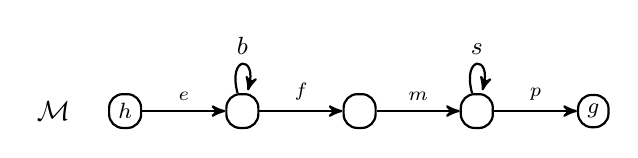
\begin{tikzpicture}[->]
    \node [state] (w1) {$h$};
    \node [left  = 0.35cm of w1] (m) {$\modults$};
    \node [state, right = of w1] (w2) {\phantom{$h$}};
    \node [state, right = of w2] (w3) {\phantom{$h$}};
    \node [state,  right = of w3] (w4) {\phantom{$h$}};
    \node [state, right = of w4] (w5) {$g$};

    \path (w1) edge[right] node [label-edge, above] {$e$} (w2)
        %(w2) edge[bend right] node [label-edge, above] {$e$} (w1)
        (w2) edge[->,loop above] node {\small$b$} (w2)
        (w2) edge[right] node [label-edge, above] {$f$} (w3)
        (w3) edge[right] node [label-edge, above] {$m$} (w4) 
        (w4) edge[->,loop above] node {\small$s$} (w4)
        (w4) edge node [label-edge, above] {$p$} (w5);
        %(w5) edge node [label-edge, below] {$e$} (w4)
            %    edge node [label-edge, above] {$w$} (w6);
\end{tikzpicture}
\begin{picture}(90,0)
    \small
\put(15,20){$\Unc(i) = \left\{
    \begin{array}{c}
    \{\mathit{ebfmsp}\}
    \end{array}
\right\}$}
\put(15,5){$\Unc(j) = \left\{
    \begin{array}{c}
    \{\mathit{ebfmsp},\mathit{ebmfsp}\}
    \end{array}
\right\}$}
\end{picture}
\end{spcenter}
The diagram shows, on the right, the set of indistinguishable plans in $\Unc(i)$ and in~$\Unc(j)$. %, containing two sets: $\plans_1=\set{ew}$ and   $\plans_2=\set{we,eew}$.
Agent $i$ knows how to bake a good cake, provided she has all the ingredients (i.e., $\modults\models\khi(h,g)$). This is because agent $i$ \emph{distinguishes} $\mathit{ebfmsp}$ as the ``good plan''. On the other hand, $j$ considers that adding milk and adding flour can be done in any order (i.e., $\mathit{ebfmsp}$ and $\mathit{ebmfsp}$ are indistinguishable), leading to $\modults\not\models\kh_j(h,g)$, as the plan
$\mathit{ebmfsp}$ is not strongly executable in the model.
\end{example}

\medskip 

%\ssparagraph{Bisimulations.} 
The notion of \emph{bisimulation} is a crucial tool for understanding the expressive power of a modal language. Here we recall the notion of bisimulation for $\KHilogic$ over \ultss~\cite{AFSVQ23report}. We start by providing some useful abbreviations.

\medskip

\begin{definition}\label{def:notation}
Let $\modults=\tup{\W,\R,\Unc,\V}$ be an \ults over \PROP, \ACT and \AGT. Take $\plans \in 2^{(\ACT^*)}$, $U, T \subseteq \W$ and $i \in \AGT$.
\begin{itemize} \itemsep 0pt
    \item Write $U \ultsExecStrat{\plans} T$ $\siffdefs$ $U \subseteq \stexec(\plans)$ and $\R_{\plans}(U) \subseteq T$.

    \item Write $U \ultsExecAgi T$ $\siffdefs$ there is $\plans \in \Unc(i)$ such that $U \ultsExecStrat{\plans} T$.
\end{itemize}
Additionally, $U \subseteq \W$ is propositionally definable in $\modults$ if and only if there is a propositional formula $\varphi$ such that $U = \truthset{\modults}{\varphi}$.
\end{definition}

\medskip

Now we are ready to introduce the notion of bisimulation for $\KHilogic$. 

\medskip 

\begin{definition}[$\KHilogic$-bisimulation]\label{def:bisim-khi}
Let $\modults = \tup{\W,\R,\Unc,\V}$ and $\modults' = \tup{\W',\R',\Unc',\V'}$ be $\ultss$.
%Take $Z \subseteq \W \times \W'$, $u \in \W$, $U \subseteq \W$, $u' \in \W'$, and $U' \subseteq \W'$.
%\begin{itemize}\itemsep 0cm
%  \item Let %$Z(u)$, $Z(U) \subseteq \W'$ as
%      \begin{nscenter}
%        \begin{tabular}{@{}c@{}}
%          $Z(u) := \setof{u' \in \W'}{uZu'}$, $Z(U) := \bigcup_{u \in U} Z(u)$.
%        \end{tabular}
%      \end{nscenter}
%
%  \item Let % $Z^{-1}(u)$, $Z^{-1}(U) \subseteq \W$ as
%      \begin{nscenter}
%        \begin{tabular}{@{}c@{}}
%          $Z^{-1}(u') := \setof{u \in \W}{uZu'}$; $Z^{-1}(U') := \bigcup_{u' \in U'} Z(u')$.
%        \end{tabular}
%      \end{nscenter}
%    \end{itemize}
A non-empty $Z \subseteq \W \times \W'$ is called an $\KHilogic$-bisimulation between $\modults$ and $\modults'$ if and only if $wZw'$ implies all of the following:
\begin{itemize} 
    \item \textbf{Atom}: $\V(w)=\V'(w')$.

    \item \textbf{$\khi$-Zig}: for any \emph{propositionally} definable $U \subseteq \W$, if $U \ultsExecAgi T$ for some $T \subseteq \W$, then there is $T' \subseteq \W'$ such that: 
%      \begin{nscenter}
%      \begin{multicols}{2}
%        \begin{enumerate}
        1) $Z(U) \ultsExecAgi T'$, and
        2) $T' \subseteq Z(T)$.
%        \end{enumerate}
%      \end{multicols}
%    \end{nscenter}

    \item \textbf{$\khi$-Zag}: % analogous to \textbf{$\khi$-Zig}.
    for any \emph{propositionally} definable $U' \subseteq \W'$, if $U' \ultsExecAgi T'$ for some $T' \subseteq \W'$, then there is $T \subseteq \W$ such that: 
%      \begin{nscenter}
%      \begin{multicols}{2}
%        \begin{enumerate}
        1) $Z^{-1}(U') \ultsExecAgi T$, and
        2) $T \subseteq Z^{-1}(T')$.
%        \end{enumerate}
%      \end{multicols}
%    \end{nscenter}

    \item \textbf{$\A$-Zig}: for all $u\in\W$ there is a $u'\in\W'$ such that $uZu'$.

    \item \textbf{$\A$-Zag}: for all $u'\in\W'$ there is a $u\in\W$ such that $uZu'$.
\end{itemize}
We write $\modults,w \bisim \modults',w'$ when there is an
$\KHilogic$-bisimulation $Z$ between $\modults$ and $\modults'$ such that
$wZw'$.
\end{definition}

\medskip

The following theorem establishes a classical adequacy result.

\medskip

\begin{theorem}[\cite{AFSVQ23report}]
Let $\modults,w$ and $\modults',w'$ be two \ultss. $\modults,w\bisim\modults',w'$ implies $\modults,w\models\varphi$ iff $\modults',w'\models\varphi$, for all $\KHilogic$-formulas $\varphi$. %Moreover, if $\modults$ and $\modults'$ are finite, the converse also holds.
\end{theorem}

\medskip 

% \ssparagraph{Axiomatization.} 

Another important element to consider is the axiom system for $\KHilogic$~\cite{AFSVQ21,AFSVQ23report}. 

\begin{table}[t]
\begin{tabular}{l@{\quad \quad  }l@{\quad}l}
\toprule
$\mbox{Axioms}$
& \axm{Taut}  & $\vdash \varphi \mbox{ for $\varphi$ a propositional tautology}$ \\
& \axm{DistA} & $\vdash \A(\varphi\ra\psi) \ra (\A\varphi \ra \A\psi)$ \\

& \axm{TA}    & $\vdash \A\varphi \ra \varphi$ \\
& \axm{4KhA}  & $\vdash \khi(\psi,\varphi) \ra \A\khi(\psi,\varphi)$ \\
& \axm{5KhA}  & $\vdash \neg\khi(\psi,\varphi) \ra \A\neg\khi(\psi,\varphi)$ \\
& \axm{KhA}   & $\vdash \left(\A(\chi \rightarrow \psi) \land \khi(\psi,\varphi) \land \A(\varphi \rightarrow \theta)\right) \rightarrow \khi(\chi, \theta)$ \\
& \axm{G} & $\vdash \khi(\varphi,\bot) \ra \kh_j(\varphi,\bot)$ \\
\midrule
\mbox{Rules}
&  \axm{MP}   & $\mbox{From $\vdash \varphi$ and $\vdash \varphi \rightarrow \psi$ infer $\vdash \psi$ }$ \\
&  \axm{NecA} & $\mbox{From $\vdash \varphi$ infer $\vdash \A\varphi$}$ \\
\bottomrule
\end{tabular}
\caption{Axiomatization $\axset_{\khi}$ for $\KHilogic$ w.r.t.\ $\ultss$.}\label{tab:khiaxiom}
\end{table}

\medskip

\begin{theorem}[\cite{AFSVQ21,AFSVQ23report}]\label{th:khi-completeness}
The axiom system from~\Cref{tab:khiaxiom} is sound and strongly complete with respect to the class of all \ultss.
\end{theorem}

\medskip

It is worth noticing two differences between the system in \Cref{tab:khiaxiom} and the one presented in~\cite{AFSVQ23report}. First, the formula $\left(\E\psi \land \khi(\psi,\varphi)\right) \rightarrow \E\varphi$, called \axm{KhE} and part of the axiom system presented in \cite{AFSVQ23report}, is omitted here. This is because it is derivable in the system, as proved below by showing the derivability of the equivalent formula $(\E\psi \wedge \khi(\psi,\varphi) \wedge \A\neg\varphi) \ra \bot$. One can start with
% , $\left(\E\psi \land \khi(\psi,\varphi) \land \A \neg\varphi \right) \rightarrow \bot$, using \axm{KhA}. %\raul{To write down the syntactic proof in detail here.}
%
% By \axm{TAUT}, it is equivalent to prove that
%
%
% \begin{equation}\label{eq:khe0}
% \vdash (\E\psi \wedge \khi(\psi,\varphi) \wedge \A\neg\varphi) \ra \bot.
% \end{equation}
%
% For this, we establish a series of implications and, using transitivity, we get \axm{KhE}. By applying \axm{TAUT}, we have that
%
\begin{spcenter}
\begin{small}
$\begin{array}{lll}
%\begin{align*}
                  & \vdash (\E\psi \wedge \khi(\psi,\varphi) \wedge \A\neg\varphi) \ra (\E\psi \wedge \khi(\psi,\varphi) \wedge \A\neg\varphi)                                 & \axm{TAUT} \\ 
  \Leftrightarrow & \vdash (\E\psi \wedge \khi(\psi,\varphi) \wedge \A\neg\varphi) \ra (\E\psi \wedge \A(\psi \ra \psi) \wedge \khi(\psi,\varphi) \wedge \A(\varphi \ra \bot)) & \axm{TAUT},\axm{NECA}
%\end{align*}
\end{array}$
\end{small}
\end{spcenter}
%
%
% \begin{equation*}
% \vdash (\E\psi \wedge \khi(\psi,\varphi) \wedge \A\neg\varphi) \ra (\E\psi \wedge \khi(\psi,\varphi) \wedge \A\neg\varphi).
% \end{equation*}
% %
% Taking \axm{TAUT} ($\vdash \neg\varphi \lra (\varphi \ra \bot)$, $\vdash \psi \ra \psi$) and \axm{NECA}, we replace $\A\neg\varphi$ by $\A(\varphi \ra \bot)$ and add $\A(\psi \ra \psi)$, which is a tautology. Thus,
% %
% \begin{equation}\label{eq:khe1}
% \vdash (\E\psi \wedge \khi(\psi,\varphi) \wedge \A\neg\varphi) \ra (\E\psi \wedge \A(\psi \ra \psi) \wedge \khi(\psi,\varphi) \wedge \A(\varphi \ra \bot)).
% \end{equation}
%
Then, by using an instance of \axm{KhA}, we have that
\begin{spcenter}
\begin{small}
$\begin{array}{lll}
%\begin{align*}
    & \vdash (\A(\psi \ra \psi) \wedge \khi(\psi,\varphi) \wedge \A(\varphi \ra \bot)) \ra (\khi(\psi,\bot)) & \\
    \Leftrightarrow &  \vdash (\E\psi \wedge \A(\psi \ra \psi) \wedge \khi(\psi,\varphi) \wedge \A(\varphi \ra \bot)) \ra (\E\psi \wedge \khi(\psi,\bot)) & \axm{TAUT} \\
    \Leftrightarrow & \vdash (\E\psi \wedge \A(\psi \ra \psi) \wedge \khi(\psi,\varphi) \wedge \A(\varphi \ra \bot)) \ra (\neg\A\neg\psi \wedge \A\neg\psi) & \mbox{Def. } \A,\E \\
    \Leftrightarrow & \vdash (\E\psi \wedge \A(\psi \ra \psi) \wedge \khi(\psi,\varphi) \wedge \A(\varphi \ra \bot)) \ra \bot & \mbox{Def. } \bot
%\end{align*}
\end{array}$
\end{small}
\end{spcenter}
%
% \begin{equation*}
% \vdash (\A(\psi \ra \psi) \wedge \khi(\psi,\varphi) \wedge \A(\varphi \ra \bot)) \ra (\khi(\psi,\bot)).
% \end{equation*}
% %
% Adding $\E\psi$ to both sides (by using an instance of \axm{TAUT}),
% %
% \begin{equation*}
% \vdash (\E\psi \wedge \A(\psi \ra \psi) \wedge \khi(\psi,\varphi) \wedge \A(\varphi \ra \bot)) \ra (\E\psi \wedge \khi(\psi,\bot)).
% \end{equation*}
% %
% By definition of $\E$ y $\A$,
% %
% \begin{equation*}
% \vdash (\E\psi \wedge \A(\psi \ra \psi) \wedge \khi(\psi,\varphi) \wedge \A(\varphi \ra \bot)) \ra (\neg\A\neg\psi \wedge \A\neg\psi).
% \end{equation*}
% %
% And by definition of $\bot$,
% %
% \begin{equation}\label{eq:khe2}
% \vdash (\E\psi \wedge \A(\psi \ra \psi) \wedge \khi(\psi,\varphi) \wedge \A(\varphi \ra \bot)) \ra \bot.
% \end{equation}
%
Given the implications proved above, \axm{KhE} follows by transitivity.

\begin{mrevised}The second difference  is the presence of the axiom \axm{G} (standing for `global' formulas).  This axiom indicates that the validity of formulas of the form $\khi(\varphi,\bot)$ is shared among all agents.  Notice that these formulas are particular, as they describe conditions that would lead to the impossible case of a goal satisfying $\bot$.  The axiom states that these formulas do not depend on the particular agent under consideration. 
%	It states that knowing how formulas that are trivially validated for an agent (in the sense that as the goal to be achieved is impossible, ), are also trivially validated for other agents. In a sense, some form of `general knowledge' is preserved between agents. 
This axiom needs to be added as a consequence of a gap in the arguments  in~\cite[Prop.~4]{AFSVQ23report}. The validity called \axm{SCond} cannot be proved without axiom \axm{G} (since the universal modality $\A$ is defined in that article as a disjunction, the last step in~\cite[Prop.~4]{AFSVQ23report} is not an equivalence). By adding \axm{G} here, we fix this issue.
\end{mrevised}

% \ssparagraph{Complexity.} 

Strong completeness of the axiomatization above is established in~\cite{AFSVQ21,AFSVQ23report} via a canonical model construction (modulo the correction just mentioned). In addition, starting from the canonical model, a careful selection function can be used to prove a small (polynomial) model property that leads to the following complexity results.

\medskip 

\begin{theorem}[\cite{AFSVQ21,AFSVQ23report}]
    The model-checking problem for $\KHilogic$ is in \Poly, while the satisfiability problem for $\KHilogic$ is \NP-complete.
\end{theorem}


\medskip

We mentioned before that the semantic interpretation for $\khi$ is `blind' to certain aspects of its witness. In fact, as the completeness proof in~\cite{AFSVQ21} shows, it cannot distinguish between the class of all arbitrary \ults and the class in which, for every agent $i$, every set in $\Unc(i)$ is a set of one-step plans (i.e., a set of basic actions). Formally, we can define this class as follows: 
\medskip 

\begin{definition}\label{def:class-m-one}
	Define $\cultsba$ (\textbf{BA} stands for `basic actions') as the class of models $\modults = \tup{\W, \R, \Unc, \V}$ in which, for all $i \in \AGT$, we have that $\plans \in \Unc(i)$ implies $\plans \subseteq \ACT$.
\end{definition}

\medskip 

$\cultsba$ (denoted $\sults$ in~\cite{AFSV22}) is a restricted class of models, which could be interpreted as a more abstract representation of the actions available to agents. In this class, every plan is modeled as a single atomic action (similar to what is done in formal verification using the so-called `path abstraction' technique, see e.g.~\cite{AbrahamJWKB10} for an example). 

\medskip	
	
\begin{proposition}
	A formula in $\KHilogic$ is valid over the class of all $\ults$ if and only if 
	it is valid over $\cultsba$.
\end{proposition}	
\medskip

The last proposition can be interpreted as a limitation on the expressivity of $\KHilogic$: since actions do not appear in its syntax, the logic is unable to distinguish between models in which witnesses are arbitrary plans and those in which they are all single atomic actions.


% Moreover, a small (polynomial) model property can be proved using selection functions and, as a corollary, the satisfiability and model checking problems of $\KHilogic$ are \NP-complete and \Poly, respectively~\cite{AFSVQ21,AFSVQ23report}. As a consequence, we have the following corollary.

% \medskip

% \begin{corollary}\label{cor:satcultsker} \carlos{Este resultado esta fuera de lugar acá. No se estiende su relación con complejidad ni su utilidad.}
% Let $\cultsfnu $ be the class of all finite \ultss such that the agents consider only basic actions distinguishable from each other (\textbf{FNU}): \raul{there are two notations, \textbf{NU} and \textbf{FNU}. Are both necessary? or are they always used together?}
% \[
% \cultsfnu := \setof{\modults}{\modults \text{ is a finite \ults and for all } i \in \AGT,\ \Unc(i) \subseteq  \setof{\set{a}}{a \in \ACT}}.
% \]
% Then, $\varphi$ is satisfiable if and only if $\varphi$ is satisfiable in $\cultsfnu$, i.e., there is $\modults \in \cultsfnu$ and $w \in \D{\modults}$ such that $\modults,w \models \varphi$.
% \end{corollary}



%\subsection{Dynamics: a brief discussion}
\medskip

After recalling the previous basic definitions and useful results of the uncertainty-based semantics for knowing how, it is time to discuss dynamic operators. The underlying idea is that of DEL: updates in the model are linked to model-changing operations, and their effect can be described by modalities whose semantic interpretation relies not only on the initial model, but also on the modified one. 

In an \ults $\tup{\W,\R,\Unc,\V}$ there is a clear distinction between ontic and epistemic information. On the one hand, the underlying \lts $\tup{\W,\R,\V}$ provides \emph{ontic}/\emph{objective} facts indicating what the actions themselves (and the plans derived from them) can do. On the other hand, the indistinguishability sets in $\Unc$ describe the \emph{epistemic} state of the agents, indicating which plans are available and the level to which the agents can discern among them. Thus, while changes in the underlying \lts can be seen as changes in a `dynamic' world to which the agents react by adjusting their epistemic state accordingly (analogous to  \emph{belief update} in the belief change literature~\cite{sep-logic-belief-revision} and to ontic changes in DEL~\cite{vanDitmarschKooi2008}), changes in the indistinguishability sets can be seen as changes in the agents' capacity to discern the world (analogous to \emph{belief revision} in the belief change literature and to epistemic changes in DEL).

The following sections explore different model-changing operations one can perform over \ultss, discussing their interpretations as well as technical results. While some examples of ontic changes will be discussed in \Cref{sec:ontic}, the main focus of the article is on epistemic updates (\Cref{sec:epistemic-basic,sec:extension}).


% pal for KH?
%For example, one of the better-known dynamic epistemic logic is \emph{Public Announcement Logic} (\PAL)~\cite{Plaza89:lopc}.  \PAL extends basic epistemic logic with an operator for public announcements which, semantically, updates a model by removing the worlds that do not satisfy the announced formula. In standard epistemic logic, this corresponds to an act of \emph{epistemic communication}: it is publicly stated that a formula $\varphi$ is the case, thus worlds stating the opposite are not longer considered as possible and deleted from the model.  Can we define similar operators in $\KHilogic$?



%In the rest of this article we will consider both ontic and epistemic updates. Some of these types of updates have been studied in~\cite{AFSV22}. In this article, we introduce a novel, more general approach, in which we enrich the logic with modalities that express explicitly that a given action can be executed. Notice that in previous works, the basic language of knowing how lacks the ability to talk explicitly about the actions. With this new feature at hand, we will be able to obtain completeness results for a dynamic language via reduction axioms.


%\section{Dynamic Knowing How Logics}
%\label{sec:dynamic}

\section{Ontic updates}
\label{sec:ontic}

This section discusses model operations updating the underlying \lts in an \ults. We discuss operations that remove states (possibly changing also the accessibility relations) and operations that directly delete edges. Within the EL setting, these two operations have a natural interpretation: they represent ways in which an agent's uncertainty changes (in this sense, the second can be seen as a generalization of the first). Here, they are reinterpreted to match what the affected model components (domain and relations) represent in the indistinguishability-based knowing how setting. In each case, we present a discussion, a modality for describing the effects of the operation, and a sound and complete axiomatization using reduction axioms, over a particular class of models.

\subsection{Removing states}
\label{sec:pal}
% Let us start by considering \PAL-like announcements in the context of knowing how logics. For the $\kh$ modality first introduced in~\cite{Wang15lori}, such an announcement would result in updating the labelled transition system in which the formula is interpreted, producing a change in the agent's abilities. In that setting, these abilities coincide with her knowledge.

%As discussed in the previous sections, our goal is to take ideas from standard epistemic logic to perform operations that update an agent's know-how.

A typical way of updating a relational model is by removing states~\cite{Plaza89:lopc,DELbook}. This model update, interpreted in the just referred literature as an announcement indicating to all agents that $\chi$ is true (hence the setting's name: \emph{public announcement logic}; \PAL), is typically described with a modal operator $[\chi]$. Given an $\ults$ $\modults=\tup{\W,\R,\Unc,\V}$, its semantic interpretation is defined as:
\[
\modults,w\models[\chi]\varphi \ \ \iff \ \  \modults,w\models\chi \mbox{ implies } \modults_{\chi},w\models\varphi,
\]
with the $\ults$ $\modults_\chi=\tup{\W_\chi,\R_\chi,\Unc_\chi,\V_\chi}$ given by
\[
\begin{array}{l@{\quad \quad \quad }l}
\W_\chi = \set{w \mid \modults,w\models\chi} & (\R_\chi)_a = \R_a \cap \W_\chi^2, \mbox{ for each } a\in\ACT \\
\V_\chi(w) = \V(w), \mbox{ for all } w\in\W_\chi & \Unc_\chi = {\Unc}.
\end{array}	
\]

Thus, $\modults_\chi$ is obtained by taking $\truthset{\modults}{\chi}$ as the new domain, then restricting relations and valuation accordingly (the indistinguishability classes $U(i)$ are left unchanged). 

A couple of remarks might be useful here. First recall that, in the \emph{knowing how} setting, states other than the evaluation point do not represent epistemic possibilities (as they do in EL), but rather situations reachable by actions. Thus, in the \emph{knowing how} setting, the elimination of some states indicates not that they are no longer \emph{possible}, but rather that they are no longer \emph{reachable}. Moreover, in the original \emph{knowing how} setting, the relations define the agents' abilities. Hence, under that semantics, removing states corresponds to both an ontic and an epistemic change: the effect of available actions changes, and hence so do the agents' abilities~\cite{Wang2016}. However, in the \ults-based semantics, relations provide only ontic information; thus, removing states produces an \emph{ontic} change that might affect, indirectly, the agents' abilities.

In the $\ults$ setting, it can be shown that the update operator adds expressivity to $\KHilogic$ (a similar result was established in~\cite{Wang2016} for the original $\lts$ setting).

\medskip 

\begin{proposition}\label{prop:pal-exp}
Adding $[\chi]$ to $\KHilogic$ increases the expressive power.
\end{proposition}

\begin{proof}
  The \ultss $\modults$ and $\modults'$ below (with $\Unc(i)=\Unc'(i)=\set{\set{a}}$, and with dashed lines indicating nodes and edges to be removed after an update with $p$) are $\KHilogic$-bisimilar (\Cref{def:bisim-khi}), and thus indistinguishable in $\KHilogic$. 
\begin{center}
    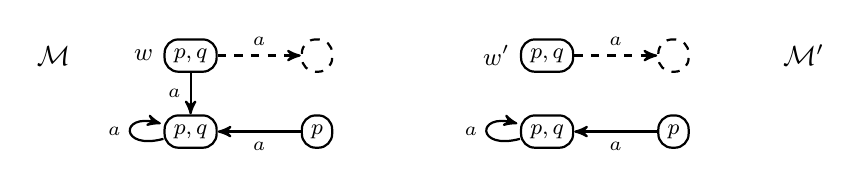
\begin{tikzpicture}[->]
      \node [state,label=left:\small$w$] (w1) {$p,q$};
      \node [state, below = of w1] (w2) {$p,q$};
      \node [state, dashed, right = of w1] (w3) {\phantom{$p$}};
      \node [state, below = of w3] (w4) {$p$};
      \node[left = of w1] (m) {$\modults$};

      \path (w1) edge node [label-edge, left] {$a$} (w2)
             (w2) edge[loop left] node [label-edge, left] {$a$} (w2)
             (w1) edge[dashed] node [label-edge, above] {$a$} (w3)
             (w4) edge node [label-edge, below] {$a$} (w2);

        \node[right = of w3] (phan) {};
        \node [state,right = of phan,label=left:\small$w'$] (w1) {$p,q$};
        \node [state, below = of w1] (w2) {$p,q$};
        \node [state, dashed, right = of w1] (w3) {\phantom{$p$}};
        \node [state, below = of w3] (w4) {$p$};
        \node[right = of w3] (mp) {$\modults'$};

        \path (w2) edge[loop left] node [label-edge, left] {$a$} (w2)
            (w1) edge[dashed] node [label-edge, above] {$a$} (w3)
            (w4) edge node [label-edge, below] {$a$} (w2);

    \end{tikzpicture}
  \end{center}
However, $\modults,w\models[p]\khi(p,q)$ whereas
$\modults',w'\not\models[p]\khi(p,q)$.
\end{proof}

A consequence of~\Cref{prop:pal-exp} is that the modality for \PAL-like updates, $[\chi]$, is not reducible to the underlying language $\KHilogic$. This makes sense: while $\KHilogic$ can express the agents' abilities to achieve certain goals from given situations (the modality $\khi$), it cannot talk about more specific properties of the courses of action on which the abilities rely. This is in contrast with what happens when these modalities are added to standard epistemic logic, where reduction axioms can be defined (see, e.g.,~\cite{DELbook}).

In such situations, the axiomatization can be approached in different ways. The `extend the basic language' method has already been explored in \cite{Wang2016}. Here, the strategy is to look for a variation of the operation, and then to restrict the setting to a particular class of models.

\medskip

\begin{definition}\label{def:annupdate}\label{def:pakhsyntax}
Let $\modults = \tup{\W, \R, \Unc, \V}$ be an \ults, and let $\chi$ be a formula. The $\ults$ $\annmodelchi = \tup{\annsemantics{\W}{\chi}, \annsemantics{\R}{\chi}, \annsemantics{\Unc}{\chi}, \annsemantics{\V}{\chi}}$ is given by:
\begin{itemize}
\item $\annsemantics{\W}{\chi} = \truthset{\modults}{\chi}$,
\item $(\annsemantics{\R}{\chi})_a = \setof{(w,v) \in \R_a}{w \in \truthset{\modults}{\chi} \text{ and } \R_a(w) \subseteq \truthset{\modults}{\chi}}$ for every $a \in \ACT$,
\item $\annsemantics{\Unc}{\chi} = \Unc$, and 
\item $\annsemantics{\V}{\chi}(w) = \V(w)$ (for all $w\in\annsemantics{\W}{\chi}$).
\end{itemize}
\smallskip
The language $\PAKHilogic$ extends $\KHilogic$ with formulas of the form $\gann{\chi}\varphi$. The semantic interpretation of the new formulas is given by
\[
	\modults,w \models \gann{\chi}\varphi \ \ \iff \ \ \modults,w \models \chi \mbox{ implies } \annmodelchi,w \models \varphi.
\]
\end{definition}

Thus, given a model $\modults$, the only difference between the standard $\modults_{\chi}$ and the just defined $\annmodelchi$ is in the definition of 
its relations. Indeed, in the former, each $(\R_\chi)_a$ restricts the original $\R_a$ to the new domain. In the latter, however, each $(\annsemantics{\R}{\chi})_a$ is defined point-wise: it is exactly as $\R_a(w)$ if all the states $\R_a(w)$ can reach will survive the operation ($\R_a(w) \subseteq \truthset{\modults}{\chi}$ implies $(\annsemantics{\R}{\chi})_a(w) = \R_a(w)$), and is empty otherwise ($\R_a(w) \not \subseteq \truthset{\modults}{\chi}$ implies $(\annsemantics{\R}{\chi})_a(w) = \emptyset$).

%\footnote{The two forms of model update discussed here resemble to the two forms of updating neighbourhood models, see~\cite{MaS18} for details.}
%Recall that a neighbourhood model~\cite{pacuit17} is given by: a non-empty domain $\W$, an atomic valuation, and a neighbourhood function $\N:\W \to 2^{2^{\W}}$, assigning a set of sets of states to each possible state. Let $U \subseteq \W$ be a non-empty set of states. On the one hand, the \emph{$U$-intersection} submodel defined in~\cite{MaS18} has $U$ as its domain, with its neighbourhood function built by restricting each set in a neighbourhood to the new domain, analogous to what $\modults_{\chi}$ (a standard announcement) does.
% On the other hand, the \emph{$U$-subset} submodel therein also has $U$ as its domain, but its neighbourhood function is built by keeping only those sets that are already a subset of the new domain, analogous to what $\annsemantics{\modults}{\chi}$ does. We argue that this second approach is more appropriate in the context of knowing how.}.

Even with this, more restricted, version of an update, the resulting logic fails to have reduction axioms: adding $\gann{\chi}$ to $\KHilogic$ increases the expressive power.

\medskip 

\begin{proposition}\label{prop:exppal}
	$\PAKHilogic$ is more expresive than $\KHilogic$ over arbitrary \ultss.
\end{proposition}

\begin{proof}
	Let $\modults$ and $\modults'$ be the single agent models depicted below, with $\Unc(i):=\set{\set{ab}}$ and $\Unc'(i):=\set{\set{a}}$:

	%\centerline{DESCOMENTAR IMAGENES ABAJO!!!}
	\begin{center}
		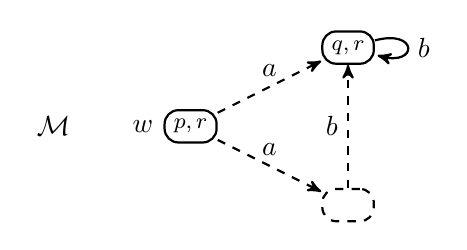
\begin{tikzpicture}[->, grow' = right, level/.style={sibling distance = 3em/#1}, level distance = 3.5em]
		\node at (0,1) [state,label=left:$w$] (p) {$p,r$} ;
		\node at (2,0) [state,dashed] (nr) {\phantom{$q,r$}};
		\node at (2,2) [state] (q) {$q,r$};
		\node[left = of p] (m) {$\modults$};

		\path (p) edge [dashed, above] node {$a$} (q);
		\path (q) edge [loop right] node [right] {$b$} (q);
		\path (p) edge [dashed,above] node {$a$} (nr);
		\path (nr) edge [dashed,left] node {$b$} (q);
		\end{tikzpicture}
		\hspace{2cm}
		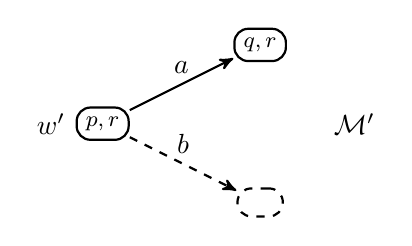
\begin{tikzpicture}[->, grow' = right, level/.style={sibling distance = 3em/#1}, level distance = 3.5em]
		\node[state] at (0,1) (p) [label=left:$w'$]{$p,r$};
		\node[state,dashed] at (2,0) (nr) {\phantom{$\neg r$}};
		\node[state] at (2,2) (q) {$q,r$};
		\node[right = 7em of p] (m) {$\modults'$};
		\path (p) edge [above] node {$a$} (q);
		\path (p) edge [dashed,above] node {$b$} (nr);
		\end{tikzpicture}
\end{center}

Both models are $\KHilogic$-bisimilar (\Cref{def:bisim-khi}); hence, they satisfy the same formulas in $\KHilogic$. However, $\modults,w \not\models \gann{r}\khi(p,q)$ since $\modults,w \models r$ and $\annmodel{r},w \not\models \khi(p,q)$, whereas $\modults',w' \models \gann{r}\khi(p,q)$ since $\modults',w' \models r$ and $\annmodel{r}',w \models \khi(p,q)$.
	%
	% \begin{nscenter}
	%   \scalebox{.7}{
	% \begin{tikzpicture}[->, grow' = right, level/.style={sibling distance = 3em/#1}, level distance = 3.5em]
	% \node[state] at (0,1) (p) [label=left:$w$]{$p,r$};
	% \node[state] at (2,2) (q) {$q,r$};
	% \path (q) edge [loop above] node {$b$} (q);
	% \end{tikzpicture}
	% \hspace{2cm}
	% \begin{tikzpicture}[->, grow' = right, level/.style={sibling distance = 3em/#1}, level distance = 3.5em]
	% \node[state] at (0,1) (p) [label=left:$w'$]{$p,r$};
	% \node[state] at (2,2) (q) {$q,r$};
	% \path (p) edge [above] node {$a$} (q);
	% \end{tikzpicture}
	%   }
	% \end{nscenter}
\end{proof}

In models $\modults$ and $\modults'$ from the above proposition, it is useful to notice the following. First, they both make the formula $\khi(p,q)$ true, their respective witnesses being $\set{ab}$ and $\set{a}$. But, as discussed, after eliminating worlds in which $r$ is false this is no longer the case: the formula fails in $\annmodel{r}$ but holds in $\annmodel{r}'$. Part of the reason is that, while the witness for the first contains a two-step plan, the witness for the second contains only one-step plans (i.e., actions). This makes a difference because, by removing intermediate steps, $\PAKHilogic$ can tell these two models apart. 

But, as mentioned before, the semantic interpretation for $\khi$ is `blind' to certain aspects of its witness. In fact, as the completeness proof shows~\cite{AFSVQ21}, it cannot distinguish between an arbitrary \ults and one in which, for every agent $i$, every plan in $\Unc(i)$ is a singleton containing only one action (i.e., a model in which $\plans \in \Unc(i)$ implies $\plans = \set{a}$ for some $a \in \ACT$). This suggests that, by restricting the class of models, one can still get agents with `the same abilities' while also stopping $\PAKHilogic$ from being able to tell $\KHilogic$-bisimilar models apart.

\medskip 

\begin{definition}\label{def:class-m-one}
Define $\cultsba$ as the class of models $\modults = \tup{\W, \R, \Unc, \V}$ in which, for all $i \in \AGT$, we have that $\plans \in \Unc(i)$ implies $\plans = \set{a}$ for some $a \in \ACT$.
\end{definition}

\medskip 

The class $\cultsba$ (denoted as $\sults$ in \cite{AFSVQ21}) constitutes a restricted class of models, which could correspond, for example, to a more abstract representation of the abilities of the agents (every plan is modelled as a single action). The reduction axioms from~\Cref{tab:palaxiom} are valid in the class of models $\cultsba$. Moreover, we can use them to eliminate announcements by iteratively replacing the innermost occurrence of a $\gann{\chi}$ modality. Thus, we get completeness for $\PAKHilogic$.

\begin{table}[t]
\begin{tabular}{l@{\quad}l}
\toprule
\axm{RAtom} & $\vdash \gann{\chi}p \leftrightarrow (\chi \implies p)$ \\
\axm{R$\neg$} & $\vdash \gann{\chi}\neg\varphi \leftrightarrow (\chi \implies \neg\gann{\chi}\varphi)$ \\
\axm{R$\vee$} & $\vdash \gann{\chi}(\varphi\vee\psi) \leftrightarrow \gann{\chi}\varphi \vee\gann{\chi}\psi$ \\
\axm{RKh} & $\vdash \gann{\chi}\khi(\varphi,\psi) \leftrightarrow (\chi \implies \khi(\chi \wedge \gann{\chi}\varphi,\chi \wedge \gann{\chi}\psi))$ \\
\axm{RE$_{\gann{}}$} & $\text{From } \vdash \varphi \leftrightarrow \psi \text{ derive } \vdash \gann{\chi}\varphi \leftrightarrow \gann{\chi}\psi$ \\
\bottomrule
\end{tabular}
\caption{Reduction axioms $\axset_{\PAKHilogic}$.}\label{tab:palaxiom}
\end{table}

\medskip 

To establish the validity of the reduction axioms, we first need to prove the following semantic properties.

\medskip 

\begin{lemma}\label{lem:palproperties} Let $\chi$ and $\varphi$ be $\PAKHilogic$-formulas; let $\modults$ be an arbitrary \ults.
	%\fer{Arbitrary models, correct?} 
	The following equalities hold:
	\begin{enumerate}
	\item $\truthset{\modults}{\gann{\chi}\varphi} = \truthset{\modults}{\neg\chi} \cup \truthset{\annmodelchi}{\varphi}$.
	\item $\truthset{\annmodelchi}{\varphi} = \truthset{\modults}{\chi \wedge \gann{\chi}\varphi}$.
	\end{enumerate}
	\end{lemma}
	
	\begin{proof}
 For Item 1, let $w \in \truthset{\modults}{\gann{\chi}\varphi}$, we have that $\modults,w \models \gann{\chi}\varphi$. Thus, $\modults,w \models \chi$ implies $\annmodelchi,w \models \varphi$, which can be rewritten as $\modults,w \models \neg\chi$ or $\annmodelchi,w \models \varphi$. Hence, $w \in \truthset{\modults}{\neg\chi} \cup \truthset{\annmodelchi}{\varphi}$. The other inclusion behaves the same way.
 
 
For Item 2, let $w \in \truthset{\annmodelchi}{\varphi}$, we have that $w \in \annsemantics{\W}{\chi} = \truthset{\modults}{\chi}$ and $w \in \truthset{\annmodelchi}{\varphi}$. Thus, $w \in \truthset{\modults}{\chi} \cap \truthset{\annmodelchi}{\varphi}$. The previous set is in the form of $(A \cap B)$. By set reasoning, it is equal to $(A \cap (A^c \cup B))$.
	In other words, the statement above is equivalent to $w \in \truthset{\modults}{\chi} \cap (\truthset{\modults}{\neg\chi} \cup \truthset{\annmodelchi}{\varphi})$. Using the result of the first item, $w \in \truthset{\modults}{\chi} \cap \truthset{\modults}{\gann{\chi}\varphi}$. Hence, $w \in \truthset{\modults}{\chi \wedge \gann{\chi}\varphi}$.
	The other inclusion behaves the same way.
	\end{proof}

\begin{lemma}\label{lemma:palkh-valid}
	The reduction axioms from~\Cref{tab:palaxiom} are valid in $\cultsba$.
	\end{lemma}
	
	\begin{proof} The proof proceeds by cases for each axiom. We will focus only on the case of $\axm{RKh}$, while the rest follow similarly as for classical $\PAL$.

	By the definition of $\gann{\chi}$, $\modults,w \models \gann{\chi}\khi(\varphi,\psi)$ iff $\modults,w \models \chi$ implies $\annmodelchi,w \models \khi(\varphi,\psi)$. Using the definition of $\khi$, $\annmodelchi,w \models \khi(\varphi,\psi)$ iff there is $\plans \in (\annsemantics{\Unc}{\chi})(i)$ with $\plans \subseteq \ACT$ s.t. $\truthset{\annmodelchi}{\varphi} \subseteq \stexec^{\annmodelchi}(\plans)$ and $(\annsemantics{\R}{\chi})_\plans(\truthset{\annmodelchi}{\varphi}) \subseteq \truthset{\annmodelchi}{\psi}$.
	By the definition of $\annmodelchi$, $(\annsemantics{\Unc}{\chi})(i)=\Unc(i)$. Using \Cref{lem:palproperties}, $\truthset{\annmodelchi}{\varphi} = \truthset{\modults}{\chi \wedge \gann{\chi}\varphi}$ and $\truthset{\annmodelchi}{\psi} = \truthset{\modults}{\chi \wedge \gann{\chi}\psi}$.
	Thus, $\annmodelchi,w \models \khi(\varphi,\psi)$ iff there is $\plans \in \Unc(i)$ with $\plans \subseteq \ACT$ s.t. $\truthset{\modults}{\chi \wedge \gann{\chi}\varphi} \subseteq \stexec^{\annmodelchi}(\plans)$ and $(\annsemantics{\R}{\chi})_\plans(\truthset{\modults}{\chi \wedge \gann{\chi}\varphi}) \subseteq \truthset{\modults}{\chi \wedge \gann{\chi}\psi}$.
	Let $a \in \plans$ and $w \in \annsemantics{\W}{\chi}$. If $w \in \truthset{\modults}{\chi \wedge \gann{\chi}\varphi}$, then:
	\begin{itemize}
		\item $(\annsemantics{\R}{\chi})_a(w) \neq \emptyset$ (since $w \in \stexec^{\annmodelchi}(a)$) and
		\item $(\annsemantics{\R}{\chi})_a(w) \subseteq \truthset{\modults}{\chi \wedge \gann{\chi}\psi}$.
	\end{itemize}
	Using \Cref{def:annupdate}, the first item is equivalent to $w \in \truthset{\modults}{\chi}$, $\R_a(w) \subseteq \truthset{\modults}{\chi}$ and $\R_a(w) \neq \emptyset$ and with this information, $(\annsemantics{\R}{\chi})_a(w) = \R_a(w)$ that is useful for the second item.
	Hence, if $w \in \truthset{\modults}{\chi \wedge \gann{\chi}\varphi}$, then:
	\begin{itemize}
		\item $w \in \truthset{\modults}{\chi}$, $\R_a(w) \subseteq \truthset{\modults}{\chi}$ and $\R_a(w) \neq \emptyset$ and
		\item $\R_a(w) \subseteq \truthset{\modults}{\chi \wedge \gann{\chi}\psi}$.
	\end{itemize}
	Note that $w \in \truthset{\modults}{\chi}$ and $\R_a(w) \subseteq \truthset{\modults}{\chi}$ are redundant as $w \in \truthset{\modults}{\chi \wedge \gann{\chi}\varphi}$ and $\R_a(w) \subseteq \truthset{\modults}{\chi \wedge \gann{\chi}\psi}$.
	With this, if $w \in \truthset{\modults}{\chi \wedge \gann{\chi}\varphi}$, then:
	\begin{itemize}
		\item $\R_a(w) \neq \emptyset$ (thus, $w \in \stexec^\modults(a)$) and
		\item $\R_a(w) \subseteq \truthset{\modults}{\chi \wedge \gann{\chi}\psi}$.
	\end{itemize}
	Since we prove for arbitrary $a \in \plans$ and $w \in \annsemantics{\W}{\chi}$, the result yields for all $a \in \plans$ and $w \in \annsemantics{\W}{\chi}$.
	Moreover, it can be generalized for all $w \in \W$ as if $w \in \truthset{\modults}{\chi \wedge \gann{\chi}\varphi}$, then $w \in \annsemantics{\W}{\chi}$.
	Now $\annmodelchi,w \models \khi(\varphi,\psi)$ iff there is $\plans \in \Unc(i)$ with $\plans \subseteq \ACT$ s.t. $\truthset{\modults}{\chi \wedge \gann{\chi}\varphi} \subseteq \stexec(\plans)$ and $\R_\plans(\truthset{\modults}{\chi \wedge \gann{\chi}\varphi}) \subseteq \truthset{\modults}{\chi \wedge \gann{\chi}\psi}$.
	This happens iff $\modults,w \models \khi(\chi \wedge \gann{\chi}\varphi,\chi \wedge \gann{\chi}\psi)$. Since for this equivalence we prove assuming $\modults,w \models \chi$, then $\modults,w \models \chi$ implies $\annmodelchi,w \models \khi(\varphi,\psi)$ iff $\modults,w \models \chi$ implies $\modults,w \models \khi(\chi \wedge \gann{\chi}\varphi,\chi \wedge \gann{\chi}\psi)$. Thus, iff $\modults,w \models \chi \implies \khi(\chi \wedge \gann{\chi}\varphi,\chi \wedge \gann{\chi}\psi)$.
	\end{proof}
	
	

Since all the reduction axioms are valid, we can state the intended result. 

\medskip 

\begin{theorem}\label{th:palcomplete}
$\axset_{\khi}$ together with the reduction axioms for $\gann{\chi}$ in~\Cref{tab:palaxiom} are a sound and strongly complete axiomatization for $\PAKHilogic$ with respect to $\cultsba$.
\end{theorem}

\begin{proof}
The result follows by the correctness of the axioms and rule from~\Cref{tab:palaxiom} stated in~\Cref{lemma:palkh-valid} (which enables us to eliminate all the occurences of a $\gann{\chi}$ modality), together with the fact that the system in~\Cref{tab:khiaxiom} is also complete with respect to $\cultsba$ (see the proof in~\cite{AFSVQ21,AFSVQ23report}).
\end{proof}


% \begin{definition}\label{def:palredtokh}
% We introduce the following reduction axioms:
% \begin{enumerate}
% \item\label{item:palredp} $\gann{\chi}p \leftrightarrow (\chi \implies p)$;
% \item\label{item:palredneg} $\gann{\chi}\neg\varphi \leftrightarrow (\chi \implies \neg\gann{\chi}\varphi)$;
% \item\label{item:palredand} $\gann{\chi}(\varphi_1\wedge\varphi_2) \leftrightarrow \gann{\chi}\varphi_1 \wedge \gann{\chi}\varphi_2$;
% \item\label{item:palredkhi} $\gann{\chi}\khi(\varphi_1,\varphi_2) \leftrightarrow (\chi \implies \khi(\chi \wedge \gann{\chi}\varphi_1,\chi \wedge \gann{\chi}\varphi_2))$.
% \end{enumerate}
% \end{definition}

To finish this discussion, we prove that the satisfiability problem for $\PAKHilogic$ is decidable at least over $\cultsba$.

\medskip 

\begin{corollary}\label{cor:palsat}
The satisfiability problem for $\PAKHilogic$ over $\cultsba$ is decidable.
\end{corollary}
\begin{proof}
Let $\varphi$ be a formula of $\PAKHilogic$. By using the reduction axioms from~\Cref{tab:palaxiom} repeatedly, $\varphi$ can be translated (in a finite amount of steps) into a formula $\varphi'$, such that $\varphi$ and $\varphi'$ are equivalent in the class $\cultsba$ (\Cref{lemma:palkh-valid}). 
Since the satisfiability problem for $\KHilogic$ is decidable (\cite{AFSVQ21,AFSVQ23report}), there is a procedure, although non-deterministic, such that in a finite amount of steps determines whether $\varphi'$ is satisfiable or not.
As a result, there are two possible outcomes:
\begin{inlineenum}
\item If $\varphi'$ is satisfiable, then it is satisfiable in the class $\cultsba$, since as established in~\cite{AFSVQ21,AFSVQ23report}, every formula is satisfiable if it satisfiable in a finite model where each $\Unc(i)\subseteq\set{\set{a} \mid a\in\ACT}$, a subclass of models strictly contained in $\cultsba$.  
% As $\cultsfnu \subseteq \cultsba$, since each $\Unc(i)$ has singleton sets of actions, then $\varphi$ is satisfiable in $\cultsba$.
\item If $\varphi'$ is not satisfiable, then clearly neither it is satisfiable in $\cultsba$. %Then, $\varphi$ is not in $\cultsba$.
\end{inlineenum}
Thus, there is a procedure that decides satisfiability of $\PAKHilogic$ over $\cultsba$. 
\end{proof}
\bigfer{Just to tie loose ends: if we work in $\cultsba$, do we have reduction axioms for the standard update operation? Or does this `trick' work only for the alternative version of the operation?}


\subsection{Removing edges}
\label{sec:aul}
% For this section we will use models $\modults = \tup{\W, \R, \Unc, \V}$ such that for all $i \in \AGT$ and all $\strategy \in \Unc(i)$, $\strategy \subseteq \ACT$ i.e. models where the knowledge every agent has are about the basic actions.
Another way to update \ltss is by modifying their relations directly while keeping the domain intact. Although there are different ways to do so (see, e.g., \cite{ArecesFH15}), in the EL context the focus has been on operations that remove edges, as this represents actions that reduce the agents' uncertainty. The \emph{arrow update logic} ($\AUL$) of~\cite{KooiR11} is a general way to do this. Its operator takes as a parameter a list of arrow specifications (triples of the form formula-action-formula). Then, an edge with label $a$ from state $w$ to state $v$ will not be deleted if and only if there is an arrow specification $(\varphi_1, a, \varphi_2)$ such that $w$ satisfies $\varphi_1$ and $v$ satisfies $\varphi_2$. 

The version of the $\AUL$ framework presented below differs from the original in two aspects. First, an arrow specification is a pair formula-formula; thus, it works for any basic action. Second, similarly as we did in~\Cref{def:annupdate}, an edge with label $a$ from state $w$ to state $v$ will not be deleted when there is an arrow specification $(\varphi_1, \varphi_2)$ such that $w$ satisfies $\varphi_1$ and \emph{all} states that can reached via $a$-edges from $w$ satisfy $\varphi_2$.
The reason for this last change relies on the same difficulties discussed with the $[\chi]$ operator. The original $\AUL$ modality has an edge-by-edge focus instead of having an group-edge one, something needed for $\khi$ formulas to have a proper translation.
The answer of whether there is a class of models compatible with this standard operator remains unclear.

\bigfer{Some questions. (1) For tying loose ends, what happens with `standard' arrow updates in the class $\cultsba$? Does the modality increase the expressivity too, thus making reduction axioms impossible? (2) Where is this variation of the arrow specification (the one that does not mention the label of the action) discussed? (3) Is axiom \axm{RJoin} taken from somewhere? If so, we can cite the reference when arguing for its validity; otherwise, some explanation might be useful.}
\bigfer{Del comentario arriba, dejo las preguntas cuya respuesta falta ser incorporada (en caso de que las queramos incorporar). Para 2 y 3, si la presentación y el axioma son originales, vale la pena mencionar eso (¿se demuestra la validez de \axm{RJoin} en el texto de DALI?)}

\medskip 

\begin{definition}
Let $\modults = \tup{\W, \R, \Unc, \V}$ be an \ults; let $U = (\theta_1,\theta'_1),\dots,(\theta_n,\theta'_n)$ be a finite list of arrow specifications with $\theta_i,\theta'_i$ formulas for every $0\leq i \leq n$. The \ults $\arrowmodelU = \tup{\W, \arrowsemantics{\R}{U}, \Unc,\V}$ is such that, for every $a\in\ACT$,
%\[
	$(\arrowsemantics{\R}{U})_a = \setof{(w,v) \in \R_a(w)}{w \in \truthset{\modults}{\bigwedge_{i=1}^n \theta_i} \text{, } \R_a(w) \subseteq \truthset{\modults}{\bigwedge_{i=1}^n \theta'_i}}$.
%\]
\end{definition}

%\bigfer{About the definition of the new model. I guess the `standard' version would be with $(\arrowsemantics{\R}{U})_a = \setof{(w,v) \in \R_a(w)}{w \in \truthset{\modults}{\bigwedge_{i=1}^n \theta_i} \text{ and } v \in \truthset{\modults}{\bigwedge_{i=1}^n \theta'_i}}$. Is that correct? If so, it seems different from the standard arrow update, at least in that the existential quantification is not explicit. Are we taking this presentation from some other source? If not, it might be worthwhile to explain it a bit.}

Note that if $w \in \truthset{\modults}{\bigwedge_{i=1}^n \theta_i}$ and $\R_a(w) \subseteq \truthset{\modults}{\bigwedge_{i=1}^n \theta'_i}$, then $(\arrowsemantics{\R}{U})_a(w) = \R_a(w)$. Moreover, $(\arrowsemantics{\R}{U})_a(w) \neq \emptyset$ iff $w \in \truthset{\modults}{\bigwedge_{i=1}^n \theta_i}$, $\R_a(w) \subseteq \truthset{\modults}{\bigwedge_{i=1}^n \theta'_i}$ and $\R_a(w) \neq \emptyset$.

\medskip

Now, the language.

\medskip

\begin{definition}\label{def:arrowsyntax}\label{def:arrowupdate}
Formulas of the language $\AUKHilogic$ are defined by the following grammar
\[
\begin{array}{lcl}
\varphi & ::= & p \mid \neg\varphi \mid \varphi\vee\varphi \mid
\khi(\varphi,\varphi) \mid \arrowbox{U}\varphi, \\
U & ::= & (\varphi,\varphi) \mid U,(\varphi,\varphi),
\end{array}
\]
with $p \in \PROP$ and $i\in\AGT$. 
%Other Boolean connectives are defined as usual. We also define
%$\arrowbox{U}\varphi := \neg \arrowbox{U} \neg\varphi$.
For the semantics, formulas already in $\KHilogic$ are interpreted as before. For the new type of formulas, 
\begin{spcenter}
	$\modults,w \models \arrowbox{U}\varphi \mbox{ iff } \arrowmodelU,w \models \varphi$.
\end{spcenter}
%Moreover, $\modults,w\models \arrowbox{U}\varphi$ iff $\modults,w\models \arrowbox{U}\varphi$ (i.e., the modality $\arrowbox{U}$ is self-dual).
\end{definition}

%\medskip 

%As in the $\PAL$ case, $\AUL$ performs ontic updates rather than epistemic %updates over $\ults$-based knowing how.

Adding the defined arrow-update modalities increases the language's expressivity.

\medskip

\begin{proposition}\label{prop:expaul}
$\AUKHilogic$ is more expressive than $\KHilogic$ over arbitrary \ultss.
\end{proposition}
\begin{proof}
By using the models from~\Cref{prop:exppal}, we have that $\modults,w \not\models [(r,r)]\khi(p,q)$ and $\modults',w' \models[(r,r)]\khi(p,q)$.
\end{proof}

Still, the reduction axioms from~\Cref{tab:aulaxiom} are valid in the class of models $\cultsba$, and we can use them to eliminate all occurrences of the $\arrowbox{U}$ modality. %Thus, we get completeness for $\AUKHilogic$.
Something worth noting is that axiom \axm{RJoin} is a semantic consequence of the definition of $\arrowbox{U}$. If we have a finite list of pair of formulas in an update $U$, we can group all formulas into a pair $(\theta,\theta')$.

\begin{table}[t]
\begin{tabular}{l@{\quad}l}
\toprule
\axm{RJoin} & $\arrowbox{U}\varphi \leftrightarrow \arrowbox{(\bigwedge_{i=1}^n \theta_i,\bigwedge_{i=1}^n \theta'_i)}\varphi$ \\
\axm{RAtom} & $\arrowbox{(\theta,\theta')}p \leftrightarrow p$ \\
\axm{R$\neg$} & $\arrowbox{(\theta,\theta')}\neg\varphi \leftrightarrow \neg \arrowbox{(\theta,\theta')}\varphi$ \\
\axm{R$\vee$} & $\arrowbox{(\theta,\theta')}(\varphi \vee \psi) \leftrightarrow \arrowbox{(\theta,\theta')}\varphi \vee \arrowbox{(\theta,\theta')}\psi$ \\
\axm{RKh} & $\arrowbox{(\theta,\theta')}\khi(\varphi,\psi) \leftrightarrow \A(\arrowbox{(\theta,\theta')}\varphi \implies \theta) \wedge \khi(\arrowbox{(\theta,\theta')}\varphi,\theta' \wedge \arrowbox{(\theta,\theta')}\psi)$ \\
\axm{RE$_U$} & $\text{From } \vdash \varphi \leftrightarrow \psi \text{ derive } \vdash \arrowbox{(\theta,\theta')}\varphi \leftrightarrow \arrowbox{(\theta,\theta')}\psi$ \\
\bottomrule
\end{tabular}
\caption{Reduction axioms $\axset_{\AUKHilogic}$ with $U = (\theta_1,\theta'_1),\dots,(\theta_n,\theta'_n)$.}\label{tab:aulaxiom}
\end{table}

\medskip 

\begin{lemma}\label{lemma:arrow-kh-valid}
	The reduction axioms from \Cref{tab:aulaxiom} are valid in $\cultsba$.
\end{lemma}

\begin{proof} The proof proceeds by cases. We only discuss $\axm{RKh}$.
	% \item For \axm{RBase}, let $U' = (\bigwedge_{i=1}^n \theta_i,\bigwedge_{i=1}^n \theta'_i) = (\alpha_1,\theta'_1)$, note that $\arrowsemantics{\W}{U} = \arrowsemantics{\W}{U'} = \W$, $\arrowsemantics{\Unc}{U} = \arrowsemantics{\Unc}{U'} = \Unc$ and $\arrowsemantics{\V}{U}(p) = \arrowsemantics{\V}{U'}(p) = \V(p)$ for every $p$. Let $a \in \ACT$, $(w,v) \in (\arrowsemantics{\R}{U})_a$ iff $w \in \truthset{\modults}{\bigwedge_{i=1}^n \theta_i}$, $\R_a(w) \subseteq \truthset{\modults}{\bigwedge_{i=1}^n \theta'_i}$.
	% Since $\truthset{\modults}{\bigwedge_{i=1}^n \theta_i} = \truthset{\modults}{\alpha_1} = \truthset{\modults}{\bigwedge_{i=1}^1 \alpha_i}$ and $\truthset{\modults}{\bigwedge_{i=1}^n \theta'_i} = \truthset{\modults}{\theta'_1} = \truthset{\modults}{\bigwedge_{i=1}^1 \theta'_i}$, $(w,v) \in (\arrowsemantics{\R}{U})_a$ iff $(w,v) \in (\arrowsemantics{\R}{U'})_a$.
	% With this, $(\arrowsemantics{\R}{U})_a = (\arrowsemantics{\R}{U'})_a$ for all $a \in \ACT$, $\arrowmodelU = \arrowmodel{U'}$ and satisfy the same formulas.
	% Thus, $\modults,w \models \arrowbox{U}\varphi$ iff $\modults,w \models \arrowbox{U'}\varphi$.
	
	% \item For \axm{RAtom}, let $U = (\theta,\theta')$, $\modults,w \models \arrowbox{U}p$ iff $\arrowmodelU,w \models p$. Since $\arrowsemantics{\V}{U}(w) = \V(w)$, $p \in \arrowsemantics{\V}{U}(w)$ iff $w \in \V(p)$. Thus, $\modults,w \models \arrowbox{U}p$ iff $\modults,w \models p$.
	
	% \item For \axm{R$\neg$}, let $U = (\theta,\theta')$, $\modults,w \models \arrowbox{U}\neg\varphi$ iff $\arrowmodelU,w \models \neg\varphi$ iff $\arrowmodelU,w \not\models \varphi$ iff $\modults,w \not\models \arrowbox{U}\varphi$ iff $\modults,w \models \neg\arrowbox{U}\varphi$.
	
	% \item For \axm{R$\vee$}, let $U = (\theta,\theta')$,
	% $\modults,w \models \arrowbox{U}(\varphi \vee \psi)$ iff $\arrowmodelU,w \models \varphi \vee \psi$ iff $\arrowmodelU,w \models \varphi$ or $\arrowmodelU,w \models \psi$ iff $\modults,w \models \arrowbox{U}\varphi$ or $\modults,w \models \arrowbox{U}\psi$ iff $\modults,w \models \arrowbox{U}\varphi \vee \arrowbox{U}\psi$.
	
	Let $U = (\theta,\theta')$, by the definition of $\arrowbox{U}$, $\modults,w \models \arrowbox{U}\khi(\varphi,\psi)$ iff $\arrowmodelU,w \models \khi(\varphi,\psi)$.
	Using the definition of $\khi$, $\arrowmodelU,w \models \khi(\varphi,\psi)$ iff there is $\plans \in (\arrowsemantics{\Unc}{U})_i$ with $\plans \subseteq \ACT$ s.t. $\truthset{\arrowmodelU}{\varphi} \subseteq \stexec^{\arrowmodelU}(\plans)$ and $(\arrowsemantics{\R}{U})_\plans(w)(\truthset{\arrowmodelU}{\varphi}) \subseteq \truthset{\arrowmodelU}{\psi}$.
	By the definition of $\arrowmodelU$, $(\arrowsemantics{\Unc}{\chi})_i=\Unc(i)$. Using the definition of $\arrowbox{U}$, $\truthset{\arrowmodelU}{\varphi} = \truthset{\modults}{\arrowbox{U}\varphi}$ and $\truthset{\arrowmodelU}{\psi} = \truthset{\modults}{\arrowbox{U}\psi}$.
	Thus, $\arrowmodelU,w \models \khi(\varphi,\psi)$ iff there is $\plans \in \Unc(i)$ with $\plans \subseteq \ACT$ s.t. $\truthset{\modults}{\arrowbox{U}\varphi} \subseteq \stexec^{\arrowmodelU}(\plans)$ and $(\arrowsemantics{\R}{U})_\plans(w)(\truthset{\modults}{\arrowbox{U}\varphi}) \subseteq \truthset{\modults}{\arrowbox{U}\psi}$.
	Let $a \in \plans$ and $w \in \arrowsemantics{\W}{U}$. If $w \in \truthset{\modults}{\arrowbox{U}\varphi}$, then:
	\begin{itemize}
	\item $(\arrowsemantics{\R}{U})_a(w) \neq \emptyset$ (since $w \in \stexec^{\arrowmodelU}(a)$) and
	\item $(\arrowsemantics{\R}{U})_a(w) \subseteq \truthset{\modults}{\arrowbox{U}\psi}$.
	\end{itemize}
	By \Cref{def:arrowupdate}, the first item is equivalent to $w \in \truthset{\modults}{\theta}$, $\R_a(w) \subseteq \truthset{\modults}{\theta'}$ and $\R_a(w) \neq \emptyset$ and hence $(\arrowsemantics{\R}{U})_a(w) = \R_a(w)$, useful for the second item.
	If $w \in \truthset{\modults}{\arrowbox{U}\varphi}$ then:
	\begin{itemize}
	\item $w \in \truthset{\modults}{\theta}$,
	\item $\R_a(w) \neq \emptyset$ (thus, $w \in \stexec^\modults(a)$),
	\item $\R_a(w) \subseteq \truthset{\modults}{\theta'}$ and $\R_a(w) \subseteq \truthset{\modults}{\arrowbox{U}\psi}$.
	\end{itemize}
	Since the first item is independent of $\plans$, we can put it outside the expression.
	It is easy to see now that $\modults,w \models \A(\arrowbox{U}\varphi \implies \theta)$ and if $w \in \truthset{\modults}{\arrowbox{U}\varphi}$, then:
	\begin{itemize}
	\item $\R_a(w) \neq \emptyset$ (thus, $w \in \stexec^\modults(a)$),
	\item $\R_a(w) \subseteq \truthset{\modults}{\theta' \wedge \arrowbox{U}\psi}$.
	\end{itemize}
	
	Since $a \in \plans$ and $w \in \arrowsemantics{\W}{U} = \W$ were arbitrary, the result yields for all $a \in \plans$ and $w \in \W$.
	Now $\arrowmodelU,w \models \khi(\varphi,\psi)$ iff $\modults,w \models \A(\arrowbox{U}\varphi \implies \theta)$ and there is $\plans \in \Unc(i)$ with $\plans \subseteq \ACT$ s.t. $\truthset{\modults}{\arrowbox{U}\varphi} \subseteq \stexec(\plans)$ and $\R_\plans(\arrowbox{U}\varphi) \subseteq \truthset{\modults}{\theta' \wedge \arrowbox{U}\psi}$.
	This happens iff $\modults,w \models (\A(\arrowbox{U}\varphi \implies \theta) \wedge \khi(\arrowbox{U}\varphi,\theta' \wedge \arrowbox{U}\psi))$ with $U = (\theta,\theta')$.
\end{proof}

As a corollary, we obtain the intended result.

\medskip 

\begin{theorem}\label{th:aulcomplete}
$\axset_{\khi}$ together with the reduction axioms for $[U]$ in~\Cref{tab:aulaxiom} are a sound and strongly complete axiomatization for $\AUKHilogic$ w.r.t. $\cultsba$.
\end{theorem}

\begin{proof}
Similar to~\Cref{th:palcomplete}.
\end{proof}

We can claim that the satisfiability problem for $\AUKHilogic$ is decidable over $\cultsba$.

\medskip 

\begin{corollary}\label{cor:aulsat}
The satisfiability problem for $\AUKHilogic$ over $\cultsba$ is decidable.
\end{corollary}
\begin{proof}
Similar to~\Cref{cor:palsat} (using~\Cref{lemma:arrow-kh-valid}).
\end{proof}


\section{Epistemic updates: a first attempt}
\label{sec:epistemic-basic} 

This section presents a first attempt at defining \emph{epistemic} updates over knowing how.  No complete axiomatization is available yet for the operators to be introduced. Instead, we  discuss their expressivity, some interesting properties, and the challenges in obtaining complete axiomatic axiomatic systems systems. 

\subsection{Removing uncertainty between two plans}
\label{sec:ref}
As it has been discussed, \ults{s} allow a natural representation of the actions that affect the abilities of an agent as well as those affecting her epistemic state. In an \ults, the crucial epistemic components are the sets $\Unc(i)$, defining the plans agent $i$ is aware of, and the degree at which she can discern among them. Thus, we can represent changes in the epistemic state of an agent by means of operations that modify $\Unc(i)$. 

\medskip

\begin{example}\label{ex:ref}
    Let $\modults$ be the \ults from \Cref{ex:cook}.
    Recall that $\modults\not\models\kh_j(h,g)$. The conflicting plan is $\mathit{ebmfsp}$, which does not lead to a good cake. Thus, if agent $j$ is able to tell apart $\mathit{ebmfsp}$ from $\mathit{ebfmsp}$ (which is the good plan), she would be able to know how to bake a good cake, provided she has the ingredients. If agent $j$ \emph{learns} that the
    order of the actions matters (so $\mathit{ebmfsp}$ is now considered distinguishable from $\mathit{ebfmsp}$), the set $\plans=\set{\mathit{ebfmsp}, \mathit{ebmfsp}}$ is split into two singleton sets (i.e., $\Unc'(j)=\set{\set{\mathit{ebfmsp}},\set{\mathit{ebmfsp}}}$, where $\Unc'(j)$ are the indistinguishability sets in the updated model). After the splitting, the agent knows how to achieve $g$ given $h$.
\end{example}

\medskip


% \begin{example}
% Let $\modults'$ be the \ults from \Cref{ex:aircraft}, but with $\Unc(i)$ containing a
% unique set of plans $\plans=\set{ew,we,eew}$. Now,
% $\modults'\not\models\khi(s,s)$. The conflicting plan is $we$, since
% from a safe zone (an $s$-state) it leads to a non-safe zone.
% Thus, if agent $i$ is able to \emph{distinguish} between $we$ and the
% rest of the plans, she would be able to know how to fly to a safe
% zone, departing from a safe zone. If agent $i$ \emph{learns} that the
% order of the actions matter (so $we$ is distinct from $ew$), she can
% split $\plans$; one way of doing this produces
% the set $\Unc(i)$ from \Cref{ex:aircraft}, where she now knows how to achieve
% $s$ given $s$.
% \end{example}

% Moreover, knowing how frameworks deal with \emph{goal-oriented} knowledge.
% So, simply removing the uncertainty between two plans might not be helpful
% (for instance, stating $\epsilon$ distinct to $we$ is not helpful in order to
% learn how to achieve $s$). However, an alternative is to look for a splitting
% of $\Unc$ that \emph{ensures} how to achieve $s$, given $s$. This approach is
% more goal-oriented, such as knowing how frameworks usually are.

% This section is devoted to explore such ideas, taking advantage of the
% facilities given by the new uncertainty-based semantics we introduced.

% One possible way of updating $\Unc$ is by adding some new plancei
% $\plan \in \ACT^*$ to $\DS{\Unc}$. An operation that takes an arbitrary {\ults}
% $\modults=\tup{\W,\R,\Unc,\V}$ and returns an {\ults}
% $\modults'=\tup{\W,\R,\Unc',\V}$ in which $\plan \in \DS{\Unc'}$ can be
% understood as an action through which the agent `becomes aware of'
% $\plan$. The actual epistemic effect of this action depends on the
% precise way in which $\plan$ is added. For example, becoming aware of
% $\plan$ while also getting to know exactly which are its effects
% (analogous to the \emph{explicit seeing} discussed in
% \cite{BenthemVel09:tdoa} in the context of awareness logic) can be
% represented by an operation in which $\plan$ gets its own strategy:
% $\Unc' := \Unc \cup \set{\set{\plan}}$. On the other hand, one could
% also add $\plan$ to an existing strategy $\plans$ (i.e.,
% $\Unc'_{\plans} := (\Unc \setminus \plans) \cup \set{\plans \cup
%   \set{\plan}}$); this might not help the agent to get new
% abilities, and it might even ruin old ones, as $\plan$ might not
% behave as the other plans that now cannot be distinguished from it.
% \footnote{In this informal discussion it has been assumed that
% $\plan \notin \DS{\Unc}$. A more general operation that does not make
% the assumption requires more care, as the condition $\plans_1,
% \plans_2 \in \Unc'$ imply $\plans_1 \cap \plans_2 =
% \emptyset$ must be preserved. Additional care is also needed when
% additional model conditions are imposed (e.g., those discussed in
% \Cref{subsec:compos}), as they also must be preserved.}

% But even if the agent does not `become aware of' new plans, she might
% still get new abilities simply by realizing that two previously
% indistinguishable plans are in fact different. The remainder of this
% section discusses two ways in which this idea can be implemented.

% The \emph{goal-oriented learning-how} modality of
% \Cref{def:goallearnsem} looks for a way to split an existing strategy
% $\plans$ to ensure that an agent knows how to make $\psi$ true when
% $\chi$ is the case.
We define an operation that eliminates uncertainty between specific
plans.  
%In an {\ults}, there might be different ways of
%making distinguishable two previously indistinguishable plans:  the
%different ways one can split a set containing both. 
First,
we introduce some notation.

%For now, we will talk about the one-agent version of $\KHilogic$ for $\ults$ models, $\KHilogic$.

\medskip

\begin{definition}
Let $\plans, \plans_1, \plans_2 \in 2^{\ACT^*}$, and $S \subseteq 2^{\ACT^*}$.  We write $\plans = \plans_1\uplus\plans_2$ iff $\plans=\plans_1\cup\plans_2$ and $\plans_1\cap\plans_2=\emptyset$.
For $\plans \in S$ and $\plans=\plans_1\uplus\plans_2$, define  $\lmodel{S}{\plans}{\set{\plans_1,\plans_2}} \subseteq 2^{\ACT^*}$ as the result of splitting, within $S$, the set of plans $\pi$ into $\pi_1$ and $\pi_2$. In other words, $\lmodel{S}{\plans}{\set{\plans_1,\plans_2}} := (S\setminus\set{\plans})\cup\set{\plans_1,\plans_2}$.
\end{definition}

\medskip

We define a relation that links sets before an update with those after the update.

\medskip

\begin{definition}\label{def:splitstr}
Let $S,S' \subseteq 2^{\ACT^*}$; and let $\plan_1,\plan_2 \in \ACT^*$ be such that $\plan_1\neq\plan_2$.
We write $\splitstr{S}{S'}{\plan_1}{\plan_2}$ if and only if either
\begin{itemize} \itemsep 0cm
\item $S' = S$ and there is no $\plans\in S$ satisfying $\set{\plan_1, \plan_2} \subseteq \plans$, or
\item $S' = \lmodel{S}{\plans}{\set{\plans_1,\plans_2}}$ for some $\plans \in S$ satisfying $\set{\plan_1, \plan_2} \subseteq \plans$, with $\plans_1, \plans_2 \in 2^{\ACT^*}$ such that
$\plans = \plans_1\uplus\plans_2$ and
$\plan_1 \in \plans_1$, $\plan_2 \in \plans_2$.
\end{itemize}
\end{definition}

\medskip

Notice that $\splitstr{}{}{\plan_1}{\plan_2}$ is serial. Moreover, if $S$ is the set of sets of plans for a given agent~$i$ in some \ults (i.e., $S=\Unc(i)$) and $S'$ is a set satisfying $\splitstr{S}{S'}{\plan_1}{\plan_2}$, then the structure resulting from replacing $S$ by $S'$ is an \ults.

\medskip

\begin{definition}
  Let $\Unc=\set{\Unc(i)}_{i\in\AGT}$ and $\Unc'=\set{\Unc'(i)}_{i\in\AGT}$ assign, to every agent in $\AGT$, a non-empty
collection of pairwise disjoint non-empty sets of plans (so $\Unc(i), \Unc'(i) \subseteq 2^{\ACT^*}$); let $\plan_1,\plan_2$ be plans in $\ACT^*$. We write $\splitstr{\Unc}{\Unc'}{\plan_1}{\plan_2}$ iff $\splitstr{\Unc(i)}{\Unc'(i)}{\plan_1}{\plan_2}$ for every $i\in\AGT$. If $\modults=\tup{\W,\R,\Unc,\V}$ is an \ults, denote by $\modults^{\Unc}_{\Unc'}$ the \ults obtained by replacing $\Unc$ by $\Unc'$.

%\fer{Minor thing, but the notation for the new model ($\modults^{\Unc}_{\Unc'}$) does not mention the plans that define the split, namely $\sigma_1, \sigma_2$}
%, and $\card{\Unc}=\card{\Unc'}$.
\end{definition}

\medskip

% The definition above guarantees there is a one-to-one correspondence between the sets in $\Unc$ and those in $\Unc'$. 
%In a sense, $\Unc'$ is a refinement of the sets in $\Unc$, for each particular agent, potentially eliminating some uncertainty for them. With these definitions in place, we introduce a new modality, $\refdiam{\plan_1}{\plan_2}$, intuitively describing an action through which all agents learn that plans $\plan_1$ and $\plan_2$ are different. The extension of $\KHilogic$ with formulas of the form $\refdiam{\plan_1}{\plan_2}\varphi$ is denoted $\Reflogic$ ({\small\textsf{Ref}} for ``refinement'').

\medskip

\begin{definition}\label{def:ref-sem}
Let $\modults=\tup{\W,\R,\Unc,\V}$ be an \ults and $w \in \W$.
For $\plan_1\neq\plan_2$,
\begin{spcenter}
$\begin{array}{l@{\ \ }c@{\ \ }l}
\modults,w\models \refdiam{\plan_1}{\plan_2}\varphi & \iffdef & \text{there is } \Unc' \text{ such that } \splitstr{\Unc}{\Unc'}{\plan_1}{\plan_2} \text{ and }  \modults^{\Unc}_{\Unc'},w \models \varphi.
\end{array}$
\end{spcenter}
As usual, we define $\refbox{\plan_1}{\plan_2}\varphi := \lnot \refdiam{\plan_1}{\plan_2}\lnot\varphi$.
\end{definition}

\medskip

Formulas like $\refdiam{\plan_1}{\plan_2}\varphi$ state that \emph{``after it is (publicly) stated that plans $\plan_1$ and $\plan_2$ are distinguishable, $\varphi$ holds''}. For instance, in~\Cref{ex:ref}, $\refdiam{\mathit{ebmfsp}}{\mathit{ebfmsp}}\kh_j(h,g)$ means that \emph{``after it is stated that $\mathit{ebmfsp}$ and $\mathit{ebfmsp}$ are different, agent $j$ knows how to bake a good cake, provided she has the ingredients''}. This modality has some natural properties. First, it is normal and serial but not deterministic (\ref{itm:distref} through \ref{itm:nodeterref} below). Moreover, it represents an idempotent action in which order does not matter and in which two consecutive applications cannot always be collapsed into a single one (\ref{itm:idempref} through \ref{itm:nocollapseref} below). 

\medskip

\begin{proposition}\label{prop:ref-normal-serial}
It follows from the semantics (\Cref{def:ref-sem}) that:
\begin{enumerate}
\item\label{itm:distref} $\models \refbox{\plan_1}{\plan_2}(\varphi \ra \psi) \ra (\refbox{\plan_1}{\plan_2}\varphi \ra
\refbox{\plan_1}{\plan_2}\psi)$.
\item\label{itm:necessitationref} If $\models \varphi$, then $\models \refbox{\plan_1}{\plan_2}\varphi$.
\item\label{itm:serialityref}  $\models \refbox{\plan_1}{\plan_2}\varphi \ra \refdiam{\plan_1}{\plan_2}\varphi$.

\item\label{itm:nodeterref}  $\not\models \refdiam{\plan_1}{\plan_2}\varphi \ra \refbox{\plan_1}{\plan_2}\varphi$.

\item\label{itm:idempref} $\models \refbox{\plan_1}{\plan_2}\refbox{\plan_1}{\plan_2}\varphi \leftrightarrow \refbox{\plan_1}{\plan_2}\varphi$.
\item\label{itm:commrefdiam} $\models \refdiam{\plan_1}{\plan_2}\refdiam{\plan_3}{\plan_4}\varphi \leftrightarrow \refdiam{\plan_3}{\plan_4}\refdiam{\plan_1}{\plan_2}\varphi$.
\item\label{itm:commrefbox} $\models \refbox{\plan_1}{\plan_2}\refbox{\plan_3}{\plan_4}\varphi \leftrightarrow \refbox{\plan_3}{\plan_4}\refbox{\plan_1}{\plan_2}\varphi$.
\item\label{itm:nocollapseref} $\modults,w \models \refdiam{\plan_1}{\plan_2}\refdiam{\plan_3}{\plan_4}\varphi$ does not imply $\exists \sigma_5, \sigma_6$ with $\modults,w \models \refdiam{\plan_5}{\plan_6}\varphi$.
\end{enumerate}
\end{proposition}

\begin{proof}
\Cref{itm:distref} follows from the $\forall$-pattern in the semantics of $\refbox{\plan_1}{\plan_2}$.
\Cref{itm:necessitationref} holds because the structure resulting from the operation is an \ults.
The seriality of $\splitstr{}{}{\plan_1}{\plan_2}$ ensures \Cref{itm:serialityref}, and its non-determinism (there is more than one way to split a set) ensures \Cref{itm:nodeterref}.
For \Cref{itm:idempref}, note that, once the sets including the given plans have been split, the operation does nothing. % Take any pointed model. If there is no agent i with $\plans \in \Unc(i)$ such that $\plan_1, \plan_2 \in \plans$, then the first case of \Cref{def:splitstr} kicks in and the operation does nothing. Otherwise, the first application will split such $\plans$, but then a further application will do nothing, as there would be no such $\plans$ left afterwards.
For \Cref{itm:commrefdiam}, there are several cases. The one we should focus on is that in which all of the involved plans are in the same set $\plans$. Since we are talking about existential modalities, a partition of $\plans$ into three parts on the left side of the equivalence can always be reproduced by the right part and viceversa. % More precisely, consider a single agent with S = { {s1, s2, s3, s4} }. Then it is possible to obtain S' = { {s1, s3}, {s2, s4} } and then S'' = { {s1, s3}, {s2, s4} }, but also to obtain S' = { {s1}, {s2, s3, s4} } and then S'' = { {s1}, {s2, s3}, {s4} }, and also S' = { {s1}, {s2, s3, s4} } and then S'' = { {s1}, {s2, s4}, {s3} }. In the very first, s1 and s3 are indistinguishable, but they are distinguishable in the very last. Then, just adjust what those plans do, to be sure their indistinguishability affects the agent's abilities
\Cref{itm:commrefbox} can be proved using \Cref{itm:commrefdiam}. Finally, for \Cref{itm:nocollapseref} it is enough to notice that, if the set of plans containing $\sigma_1, \sigma_2$ is different from that containing $\sigma_3, \sigma_4$, then the two actions refine two indistinguishability sets, something that cannot be replicated by a single application.
\end{proof}

The new dynamic modality preserves knowing how information when it refers to propositional formulas (\Cref{itm:preservesknowledge} below).  And it is not trivial, in the sense that it leads to an increase of knowledge in certain situations (\Cref{itm:gainsknowledge}).

\medskip

\begin{proposition}\label{prop:ref-preserves-gains}
Let $\varphi,\psi$ be propositional formulas; take $\plan_1,\plan_2\in\ACT^*$ with $\plan_1\neq\plan_2$.
\begin{enumerate}
\item\label{itm:preservesknowledge} $\models \khi(\varphi,\psi) \ra \refbox{\plan_1}{\plan_2}\khi(\varphi,\psi)$.
\item\label{itm:gainsknowledge} If $\varphi$ and $\psi$ are satisfiable, then $\neg\khi(\varphi,\psi) \wedge \refdiam{\plan_1}{\plan_2}\khi(\varphi,\psi)$ is satisfiable.
\end{enumerate}
\end{proposition}
\begin{proof}
For \Cref{itm:preservesknowledge}, suppose $\modults, w \models \khi(\varphi,\psi)$.
Then there is $\plans \in \Unc(i)$ s.t. $\truthset{\modults}{\varphi} \subseteq \stexec(\plans)$ and $\R_\plans(\truthset{\modults}{\varphi}) \subseteq \truthset{\modults}{\psi}$.
Let $\plan_1$, $\plan_2$ $\in \ACT^*$.
If $\plan_1 \not\in \plans$ or $\plan_2 \not\in \plans$, then $\plans$ does not change and is still the witness for $\khi(\varphi,\psi)$.
If, however, $\plan_1,\plan_2 \in \plans$, there will be a partition of $\plans$, $\set{\plans_1,\plans_2}$ such that $\splitstr{\Unc(i)}{\lmodel{\Unc(i)}{\plans}{\set{\plans_1,\plans_2}}}{\plan_1}{\plan_2}$.
But this does not cause any problem since $\truthset{\modults}{\varphi} \subseteq \stexec(\plans) \subseteq \stexec(\plans_k)$ and $\R_{\plans_k}(\truthset{\modults}{\varphi}) \subseteq \R_\plans(\truthset{\modults}{\varphi}) \subseteq \truthset{\modults}{\psi}$, for $k\in\set{1,2}$.
Here, agent $i$ knew how to %do a certain task under a restricted condition from the
go from $\varphi$-states to $\psi$-states via $\plans$.
Weakening such a $\plans$ by splitting it into two pieces still works, allowing the agent to choose between $\plans_1$ or $\plans_2$ as her next witness.
Since all the cases for $\plan_1$ and $\plan_2$ are covered, we can conclude that $\modults,w\models \refbox{\plan_1}{\plan_2}\khi(\varphi,\psi)$.

For \Cref{itm:gainsknowledge}, let $\plan_1 \neq \plan_2$, and let $\modults=\tup{\set{u,v},\R,\set{\Unc(i)},\V}$ be a model such that
\begin{itemize}
\item $\modults,u \models \varphi$ and $\modults,v \models \psi$;
\item $\R_{\plan_1[1]} = \set{(u,v),(v,v)}$ and $\R_{\plan_1[j]} = \set{(v,v)}$ for all $j = 2, \dots, \card{\plan_1}$;
\item $\R_{\plan_2[k]} = \emptyset$ for some $k = 1, \dots, \card{\plan_2}$ (since $\plan_1 \neq \plan_2$); and
\item $\Unc(i) = \set{\set{\plan_1,\plan_2}}$.
\end{itemize}

The model $\modults$ is depicted below (the plan $\plan_2$ is omitted):

\begin{center}
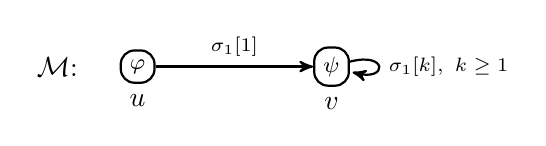
\begin{tikzpicture}[->, grow' = right]
\node (m) {$\modults$:};
\node [state, right = 0.4cm of m, label=below:$u$] (u) {$\varphi$};
\node [state, right = 2cm of u, label=below:$v$] (v) {$\psi$};

\path (u) edge[right] node [label-edge, above] {$\plan_1[1]$} (v);
\path (v) edge[loop right] node [label-edge] {$\plan_1[k], \ k \geq 1$} (v);
\end{tikzpicture}
\end{center}

Since $u \not\in \stexec(\plan_2) = \stexec(\set{\plan_1,\plan_2})$, we have that $\modults \models \neg\khi(\varphi,\psi)$.
However, $\modults \models \refdiam{\plan_1}{\plan_2}\khi(\varphi,\psi)$ as $\splitstr{\set{\set{\plan_1,\plan_2}}}{\set{\set{\plan_1},\set{\plan_2}}}{\plan_1}{\plan_2}$ and $\set{\plan_1}$ acts as a witness.
\end{proof}
% \bigfer{In the previous proposition, the standard problem in these cases is that $\truthset{\modults}{\varphi}$ and $\truthset{\modults^{\Unc}_{\Unc'}}{\varphi}$ might be different (because the model changes). Asking for $\varphi$ and $\psi$ to be propositional guarantees that $\truthset{\modults}{\varphi}$ and $\truthset{\modults^{\Unc}_{\Unc'}}{\varphi}$ coincide (as valuations do not change). But arguing whether that holds for arbitrary $\varphi$ (if that is indeed the case) might require more care.}

However, \Cref{itm:preservesknowledge} in \Cref{prop:ref-preserves-gains} fails for arbitrary formulas.

\medskip

\begin{example}
Consider again~\Cref{ex:cook}, and let $\theta = \kh_j(h,g)$. Since $\modults \not\models \theta$, then we have $\modults \models \kh_j(\theta,\neg \theta)$. Since $\modults\models\refdiam{\mathit{ebmfsp}}{\mathit{ebfmsp}}\theta$, it cannot be the case that  $\modults \models \refdiam{\mathit{ebmfsp}}{\mathit{ebfmsp}}\kh_j(\theta,\neg \theta)$. Thus, $\modults \not\models \kh_j(\theta,\neg \theta) \ra \refbox{\mathit{ebmfsp}}{\mathit{ebfmsp}}\kh_j(\theta,\neg \theta)$, falsifying \Cref{itm:preservesknowledge} for arbitrary formulas.
\end{example}

\medskip

The new modality can explicitly refer to plans. Thus, as it could be expected, it adds expressivity w.r.t.\ the basic knowing how logic. 

\medskip

\begin{proposition}\label{prop:expref}
$\Reflogic$ is more expressive than $\KHilogic$.
\end{proposition}
\begin{proof}
%We need to display two $\KHilogic$-bisimilar  that can be distinguished by an $\Reflogic$-formula.
%Consider the \ultss $\modults$ and $\modults'$ below:
The single agent \ultss models $\modults$ and $\modults'$ depicted below (with $\Unc(i):=\set{\set{a}}$ and $\Unc'(i):=\set{\set{a,b}}$) are $\KHilogic$-bisimilar; thus, they satisfy the same formulas in $\KHilogic$. 
\begin{center}
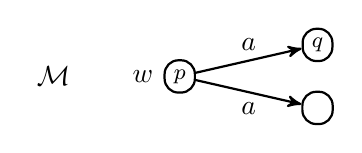
\begin{tikzpicture}[->, grow' = right, level/.style={sibling distance = 2em/#1}, level distance = 1.5em]
\node[state] at (0,1) (p) [label=left:$w$]{$p$};
\node[left = of p] (m) {$\modults$};
\node[state] at (1.75,0.6) (nq) {\phantom{$p$}};
\node[state] at (1.75,1.4) (q) {$q$};
\path (p) edge [above] node {$a$} (q);
\path (p) edge [below] node {$a$} (nq);
\end{tikzpicture}
\hspace{2cm}
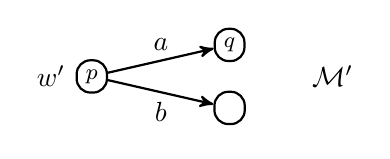
\begin{tikzpicture}[->, grow' = right, level/.style={sibling distance = 2em/#1}, level distance = 3.5em]
    \node[state] at (0,1) (p) [label=left:$w'$]{$p$};
    \node[state] at (1.75,0.6) (nq) {\phantom{$p$}};
\node[state] at (1.75,1.4) (q) {$q$};
\path (p) edge [above] node {$a$} (q);
\path (p) edge [below] node {$b$} (nq);
\node[right = 7em of p] (m) {$\modults'$};
\end{tikzpicture}
\end{center}
Still, $\modults,w \not\models \refdiam{a}{b}\khi(p,q)$ since $\splitstr{\Unc(i)}{\Unc(i)}{a}{b}$, % then $\Unc=\overline{\Unc}$,
whereas $\modults',w' \models \refdiam{a}{b}\khi(p,q)$, since there is $\Unc''(i)=\set{\set{a},\set{b}}$ such that $\splitstr{\Unc'(i)}{\Unc''(i)}{a}{b}$.
%
% \begin{nscenter}
% \begin{tabular}{@{}l@{}l@{}}
% \begin{tabular}{@{}c}
% \begin{tikzpicture}[->, grow' = right, level/.style={sibling distance = 3em/#1}, level distance = 3.5em]
%
% \node [state, label = {[label-state]left:$w$}] (r) {$p$}
% child { node [state] {$p$}
%         child { node [state] (n1) {$p$}
%                 edge from parent node [label-edge, above] {$a$} }
%         child { node [state] (n2) {}
%                 edge from parent node [label-edge, below] {$a$} }
%     edge from parent node [label-edge, above] {$a$} }
% child { node [state] {}
%         child { node [state] (n3) {$p$}
%                 edge from parent node [label-edge, above] {$a$} }
%         child { node [state] (n4) {}
%                 edge from parent node [label-edge, below] {$a$} }
%     edge from parent node [label-edge, below] {$a$} };
%
% \node[right = 0.5em of n1.center] {$\cdots$};
% \node[right = 0.5em of n2.center] {$\cdots$};
% \node[right = 0.5em of n3.center] {$\cdots$};
% \node[right = 0.5em of n4.center] {$\cdots$};
%
% \node[node distance = 0.1em and 2em, above = 1em of r] {$\modults$};
% \end{tikzpicture}
% \end{tabular}
% &
% \begin{tabular}{c@{}}
% \begin{tikzpicture}[->, grow' = right, level/.style={sibling distance = 3em/#1}, level distance = 3.5em]
% \node [state, label = {[label-state]left:$w'$}] (r) {$p$}
% child { node [state] {$p$}
%         child { node [state] (n1) {$p$}
%                 edge from parent node [label-edge, above] {$a$} }
%         child { node [state] (n2) {}
%                 edge from parent node [label-edge, below] {$b$} }
%     edge from parent node [label-edge, above] {$a$} }
% child { node [state] {}
%         child { node [state] (n3) {$p$}
%                 edge from parent node [label-edge, above] {$a$} }
%         child { node [state] (n4) {}
%                 edge from parent node [label-edge, below] {$b$} }
%     edge from parent node [label-edge, below] {$b$} };
%
% \node[right = 0.5em of n1.center] {$\cdots$};
% \node[right = 0.5em of n2.center] {$\cdots$};
% \node[right = 0.5em of n3.center] {$\cdots$};
% \node[right = 0.5em of n4.center] {$\cdots$};
%
% \node[node distance = 0.1em and 2em, above = 1em of r] {$\modults'$};
% \end{tikzpicture}
% \end{tabular}
% \end{tabular}
% \end{nscenter}
%
% They are binary trees, with each node forking in $p$ and $\neg p$. Consider a single agent $i$.
% The respective sets of sets of plans are $\Unc(i)=\set{\set{a}}$ and $\Unc'(I)=\set{\set{a,b}}$.
% It is clear that $\modults,w\bisim\modults',w'$, but $\modults,w \not\models \refdiam{a}{b}\khi(p,p)$ whereas $\modults',w' \models \refdiam{a}{b}\khi(p,p)$.
\end{proof}

We conclude by showing that \emph{uniform substitution} fails in $\Reflogic$. Uniform substitution establishes that given a valid formula $\varphi$, we can uniformly replace any propositional symbol appearing in $\varphi$ by an arbitrary formula, and obtain a valid formula.  
\begin{mrevised}
The property fails for many dynamic logics.  For example, the logics $\PAKHilogic$ and $\AUKHilogic$ introduced in the previous section are not closed under uniform substitution.  Particular cases where the property fails are the respective $\axm{RAtom}$ axioms, which are valid for $p \in \PROP$ but validity is not preserved under arbitrary substitutions. 

Failure of uniform substitution is not so problematic in the cases of $\PAKHilogic$, $\AUKHilogic$ over the class $\cultsba$ and, more generally, for dynamic logics with 
reduction axioms. In these cases, the dynamic modalities can be eliminated to obtain an equivalent formula which is closed under substitutions. The case of $\Reflogic$ is more complex. Its increased expressive power w.r.t.\ $\KHilogic$ implies that reduction axioms cannot be defined.  This, in addition to the failure of uniform substitution, indicates that complete axiomatizations might be difficult to find. 
\end{mrevised}

\medskip

\begin{proposition}\label{prop:substitution-ref}
    Uniform substitution fails in $\Reflogic$.
\end{proposition}

\begin{proof}
The formula $p\to\refdiam{a}{b}p$ is valid for $p$ a propositional symbol, since $\refdiam{a}{b}$ does not change the valuation. Consider the model below, with $\Unc(i):=\set{\set{a,b}}$:
\begin{center}
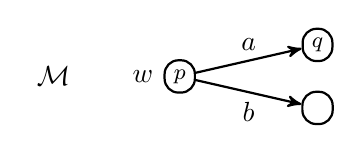
\begin{tikzpicture}[->, grow' = right, level/.style={sibling distance = 2em/#1}, level distance = 1.5em]
    \node[state] at (0,1) (p) [label=left:$w$]{$p$};
    \node[left = of p] (m) {$\modults$};
    \node[state] at (1.75,0.6) (nq) {\phantom{$p$}};
    \node[state] at (1.75,1.4) (q) {$q$};
    \path (p) edge [above] node {$a$} (q);
    \path (p) edge [below] node {$b$} (nq);
    \end{tikzpicture} 
\end{center}
Consider now the substitution of $p$ by $\neg\khi(p,q)$ in the formula above. The resulting formula is $\neg\khi(p,q)\to\refdiam{a}{b}\neg\khi(p,q)$. It is clear that $\modults\models\neg\khi(p,q)$, but $\modults\not\models\refdiam{a}{b}\neg\khi(p,q)$. Thus, $\neg\khi(p,q)\to\refdiam{a}{b}\neg\khi(p,q)$ is not valid.
\end{proof}

It is well-known that the lack of uniform substitution in many dynamic logics poses a serious challenge in obtaining complete axiomatizations (see, e.g.,~\cite{HoHoIc11}). This issue has been dealt with in, e.g.,~\cite{BenthemMZ2022,BenthemLSY22}, for sabotage modal logics.
Therein, hybrid logic machinery is used to obtain complete axiomatic systems. This approach seems difficult to apply in our setting, as the language is unable to talk about the actual plans witnessing a formula. We will take a different path in~\Cref{sec:extension}.

% \begin{definition}[Reachability]\label{def:reachability}
% Let $\modults = \tup{\W,\R,\Unc,\V}$ be \ultss, $\Unc'$ is finitely reachable from $\Unc$ if there is a finite sequence of $\Unc(k)$, $\plan_1^k$ and $\plan_2^k$ for $k=1,...,n$ such that $\splitstr{\Unc(k)}{\Unc(k+1)}{\plan_1^k}{\plan_2^k}$, $\Unc(1)=\Unc$ and $\Unc(n)=\Unc'$.
% The set of all finitely reachable $\Unc'$ sets from $\Unc$ is denoted as $\REACH{\Unc}$.
% \end{definition}
%
% Note that $\Unc \in \REACH{\Unc}$ as if $\plan_1 = \plan_2$, there would be no $\plans$ such that can be partitioned in two and have $\plan_1$ in each partition.

% \begin{definition}[$\Reflogic$-bisimulation]\label{def:bisim-ref}
% Let $\modults$ and $\modults'$ be two \ultss, with domains $\W$ and $\W'$, resp; take $Z \subseteq (\W \times \REACH{\Unc}) \times (\W' \times \REACH{\Unc'})$.
% \begin{itemize}\itemsep 0cm
% \item For $u \in \W$, $\Unc(0) \in \REACH{\Unc}, \Unc'(0) \in \REACH{\Unc'}$
% and $U \subseteq \W$, define
%
% \begin{nscenter}
% \begin{small}
% \begin{tabular}{@{}c@{}}
% $Z(u,\Unc(0),\Unc'(0)) := \csetsc{u' \in \W'}{(u,\Unc(0))Z(u',\Unc'(0))}$;
% $Z(U,\Unc(0),\Unc'(0)) := \bigcup_{u \in U} Z(u,\Unc(0),\Unc'(0))$.
% \end{tabular}
% \end{small}
% \end{nscenter}
%
% \item For $u' \in \W'$, $\Unc'(0) \in \REACH{\Unc'},\Unc(0) \in \REACH{\Unc}$
% and $U' \subseteq \W'$, define
%
% \begin{nscenter}
% \begin{small}
% \begin{tabular}{@{}c@{}}
% $Z^{-1}(u',\Unc'(0),\Unc(0)) := \csetsc{u \in \W}{(u,\Unc(0))Z(u',\Unc'(0))}$;
% $Z^{-1}(U',\Unc'(0),\Unc(0)) := \bigcup_{u' \in U'} Z(u',\Unc'(0),\Unc(0))$.
% \end{tabular}
% \end{small}
% \end{nscenter}
%
% \end{itemize}
% \end{definition}

% \begin{definition}[Submodel]\label{def:submodel}
% Let $\modults = \tup{\W,\R,\Unc,\V}$ and $\modults' = \tup{\W',\R',\Unc',\V'}$ be \ultss, $\modults'$ is a submodel of $\modults$ if $\W' = \W$, $\R' = \R$, $\V' = \V$ and $\Unc'$ is finitely reachable from $\Unc$ (i.e. $\Unc' \in \REACH{\Unc}$).
% We write $\modults' \subseteq \modults$ if $\modults'$ is a submodel of $\modults$.
% Moreover, we denote this model as $\modults_{\Unc'}$.
% \end{definition}

% \begin{definition}\label{def:notation-ref}
% Let $\modults=\tup{\W,\R,\Unc,\V}$ be an \ults.
% For $\plans \in 2^{\ACT^*}$, $U,T \subseteq \W$,
% \begin{itemize} \itemsep 0cm
% \item write $U \ultsExecStrat{\plans}_{\Unc} T$ {\;\iffdef\;}
% $U \subseteq \stexec^\modults(\plans)$ and $T = \R_{\plans}(U)$;
% \item write $U \ultsExec_{\Unc} T$ {\;\iffdef\;}
% if there is $\plans \in \Unc$ such that $U \ultsExecStrat{\plans}_{\Unc} T$.
% \end{itemize}
% \textcolor{red}{Additionally, we say that $U \subseteq \W$ is $\Reflogic$-propositionally definable in $\modults$ if and only if there
% is an $\Reflogic$-propositional formula $\varphi$ such that $U = \truthset{\modults}{\varphi}$.}
%
% \bigraul{creo que la definicion abajo no es correcta; no deberiamos tomar siempre al nivel 0, si no que tenemos que tomar en $n$, y un update me mueve a $n+1$, mientras que $\khi$ trabajar en nivel $n$ en ambos lados}
% \end{definition}
% \begin{definition}
% A non-empty $Z \subseteq (\W \times \REACH{\Unc}) \times (\W' \times \REACH{\Unc'})$ is called an $\Reflogic$-bisimulation between $\modults$ and $\modults'$ if and only if $(w,\Unc(0))Z(w',\Unc'(0))$ implies:
% \begin{itemize} \itemsep 0cm
% \item \textbf{Atom}: $\V(w)=\V'(w')$.
%
% \item \textbf{$\kh$-Zig}: for any \textcolor{red}{\emph{propositionally} definable} $U \subseteq \W$, if $U \ultsExec_{S_0} T$ for some $T \subseteq \W$, then there is $T' \subseteq \W'$ s.t.
% \begin{ltabular}{l@{\;}l@{\qquad\qquad}l@{\;}l}
% \ITM{i}  & $Z(U,\Unc(0),\Unc'(0)) \ultsExec_{\Unc'(0)} T'$, and &
% \ITM{ii} & $T' \subseteq Z(T,\Unc(0),\Unc'(0))$.
% \end{ltabular}
%
% \item \textbf{$\kh$-Zag}: for any \textcolor{red}{\emph{propositionally} definable} $U' \subseteq \W'$, if $U' \ultsExec_{\Unc'(0)} T'$ for some $T' \subseteq \W'$, then there is $T \subseteq \W$ s.t.
% \begin{ltabular}{l@{\;}l@{\qquad\qquad}l@{\;}l}
% \ITM{i}  & $Z^{-1}(U',\Unc'(0),\Unc(0)) \ultsExec_{\Unc(0)} T$, and &
% \ITM{ii} & $T \subseteq Z^{-1}(T',\Unc'(0),\Unc(0))$.
% \end{ltabular}
%
% \item \textbf{$\A$-Zig}: for all $u$ in $\W$ there is a $u'$ in $\W'$ such that $(u,\Unc(0))Z(u',\Unc'(0))$.
%
% \item \textbf{$\A$-Zag}: for all $u'$ in $\W'$ there is a $u$ in $\W$ such that $(u,\Unc(0))Z(u',\Unc'(0))$.
%
% \item \textbf{$\refdiam{\plan_1}{\plan_2}$-Zig}:
% for all $\plan_1$, $\plan_2$ in $\ACT^*$ if there is a $\overline{\Unc}(0)$ in $\REACH{\Unc}$ such that $\splitstr{\Unc(0)}{\overline{\Unc}(0)}{\plan_1}{\plan_2}$, then there is a $\overline{\Unc}'_0$ in $\REACH{\Unc'}$ such that $\splitstr{\Unc'(0)}{\overline{\Unc}'_0}{\plan_1}{\plan_2}$ and $(w,\overline{\Unc}(0))Z(w',\overline{\Unc}'_0)$.
%
% \item \textbf{$\refdiam{\plan_1}{\plan_2}$-Zag}:
% for all $\plan_1$, $\plan_2$ in $\ACT^*$ if there is a $\overline{\Unc}'_0$ in $\REACH{\Unc'}$ such that $\splitstr{\Unc'(0)}{\overline{\Unc}'_0}{\plan_1}{\plan_2}$, then there is a $\overline{\Unc}(0)$ in $\REACH{\Unc}$ such that $\splitstr{\Unc(0)}{\overline{\Unc}(0)}{\plan_1}{\plan_2}$ and $(w,\overline{\Unc}(0))Z(w',\overline{\Unc}'_0)$.
% \end{itemize}
%
% We write $\modults,w \bisim_\Reflogic \modults',w'$ when there is an $\Reflogic$-bisimulation $Z$ between $\modults$ and $\modults'$ such that $(w,\Unc)Z(w',\Unc')$.
% \end{definition}
%
% \begin{definition}[$\Reflogic$-equivalence]\label{def:equiv-ref}
% The pointed \ultss $\modults, w$ and $\modults', w'$ are \emph{$\Reflogic$-equivalent} (written $\modults, w \modequiv_\Reflogic \modults', w'$) if and only if $\modults, w \models \varphi$ iff $\modults', w' \models \varphi$ for all $\varphi \in \Reflogic$.
% \end{definition}
%
% \begin{theorem}[Invariance for $\Reflogic$]\label{th:refbisim-to-refequiv}
% Let $\modults, w$ and $\modults', w'$ be pointed \ultss.
% Then, $\modults,w \bisim_\Reflogic \modults', w' \text{ implies }\modults,w \modequiv_\Reflogic \modults',w'$.
% \end{theorem}
% \begin{proof}
% The proof of $\Reflogic$-equivalence is by structural induction on $\Reflogic$-formulas.
% The goal is to probe that $(u,\Unc(0))Z(u',\Unc(0)')$ (with the induced submodels $\modults_{\Unc(0)} \subseteq \modults$ and $\modults_{\Unc(0)'}' \subseteq \modults'$) implies $\modults_{\Unc(0)},u \modequiv_\Reflogic \modults_{\Unc(0)'}',u'$.
% The cases for atomic propositions and Boolean operators are standard.
%
% For formulas of the form $\kh(\psi,\varphi)$, we have a similar approach as in Theorem \ref{th:khbisim-to-khequiv}.
% Suppose $u \in \truthset{\modults_{\Unc(0)}}{\kh(\psi,\varphi)}$; then, there is $\plans \in \Unc(0)$
% s.t. $\truthset{\modults_{\Unc(0)}}{\psi} \ultsExecStrat{\plans}_{\Unc(0)} T$ and
% $T=\R_{\plans}(\truthset{\modults_{\Unc(0)}}{\psi}) \subseteq \truthset{\modults_{\Unc(0)}}{\varphi}$.
% First, note how $Z(\truthset{\modults_{\Unc(0)}}{\psi},\Unc(0),\Unc(0)') = \truthset{\modults_{\Unc(0)'}'}{\psi}$.
% Indeed, $(\subseteq)$ if $v' \in Z(\truthset{\modults_{\Unc(0)}}{\psi},\Unc(0),\Unc(0)')$, then there is $v \in \truthset{\modults_{\Unc(0)}}{\psi}$ such that $(v,\Unc(0))Z(v',\Unc(0)')$; thus, from IH we have $v' \in \truthset{\modults_{\Unc(0)'}'}{\psi}$.
% $(\supseteq)$ If $v' \in \truthset{\modults_{\Unc(0)'}'}{\psi}$, by $\A$-Zag there is $v$ with $(v,\Unc(0))Z(v',\Unc(0)')$; thus, from IH we have $v \in \truthset{\modults_{\Unc(0)}}{\psi}$.
% Hence, $v' \in Z(\truthset{\modults_{\Unc(0)}}{\psi},\Unc(0),\Unc(0)')$.
%
% The set \textcolor{red}{$\truthset{\modults_{\Unc(0)}}{\psi}$ is $\Reflogic$-definable, (we are not sure if it is also propositionally definable; if not, we can redefine bisimulations; from here the proof assumes it is the case) and thus propositionally definable}. \raul{creo que como la modalidad dinamica es global, esto deberia valer de todos modos, pero en el modelo adecuado}
% Moreover, there are $\plans \in \Unc(0)$ and $T \subseteq \W$ such that $\truthset{\modults_{\Unc(0)}}{\psi} \ultsExecStrat{\plans}_{\Unc(0)} T$, so $\truthset{\modults_{\Unc(0)}}{\psi} \ultsExec_{\Unc(0)} T$.
% Then, from the latter and clause $\kh$-Zig, there is $T' \subseteq \W'$ such that
%
% \begin{enumerate}
% \item $Z(\truthset{\modults_{\Unc(0)}}{\psi},\Unc(0),\Unc(0)') \ultsExec_{\Unc(0)'} T'$ (so $\truthset{\modults_{\Unc(0)'}'}{\psi} \ultsExec_{\Unc(0)'} T'$, by the result above), and
% \item\label{itm:ii} $T' \subseteq Z(T,\Unc(0),\Unc(0)')$.
% \end{enumerate}
%
% Now, we know that $T \subseteq \truthset{\modults_{\Unc(0)}}{\varphi}$, that is, $v \in T$ implies $v \in \truthset{\modults_{\Unc(0)}}{\varphi}$.
% But then, by IH, $v \in T$ and $(v,\Unc(0))Z(v',\Unc(0)')$ implies $v' \in \truthset{\modults_{\Unc(0)'}'}{\varphi}$.
% Thus, $Z(T,\Unc(0),\Unc(0)') \subseteq \truthset{\modults_{\Unc(0)'}'}{\varphi}$.
% This, together with \itm{\ref{itm:ii}} from the previous paragraph, yields $T' \subseteq \truthset{\modults_{\Unc(0)'}'}{\varphi}$.
% Thus, we have both $\truthset{\modults_{\Unc(0)'}'}{\psi} \ultsExec_{\Unc(0)'} T'$ (there is an strongly executable strategy which, from $\psi$-worlds, reaches only $T'$-worlds) and $T' \subseteq \truthset{\modults_{\Unc(0)'}'}{\varphi}$ (every $T'$-world satisfies $\varphi$); hence, $u' \in \truthset{\modults_{\Unc(0)}'}{\kh(\psi,\varphi)}$.
%
% The direction from $u' \in \truthset{\modults_{\Unc(0)'}'}{\kh(\psi,\varphi)}$ to $u \in \truthset{\modults_{\Unc(0)}}{\kh(\psi,\varphi)}$ follows a similar argument, using $\A$-Zig and $\kh$-Zag instead.
%
% For the case $\refdiam{\plan_1}{\plan_2}\varphi$, suppose $\modults_{\Unc(0)},u \models \refdiam{\plan_1}{\plan_2}\varphi$.
% Then, there is $\overline{\Unc}(0) \in \REACH{\Unc}$ s.t. $\splitstr{\Unc(0)}{\overline{\Unc}(0)}{\plan_1}{\plan_2}$ and $\modults^{\Unc(0)}_{\overline{\Unc}(0)} = \modults_{\overline{\Unc}(0)},u \models \varphi$.
% Then, by $\refdiam{\plan_1}{\plan_2}$-Zig, there is a
% $\overline{\Unc}(0)' \in \REACH{\Unc'}$ such that $\splitstr{\Unc(0)'}{\overline{\Unc}(0)'}{\plan_1}{\plan_2}$ and $(u,\overline{\Unc}(0))Z(u',\overline{\Unc}(0)')$.
% By IH, $\modults'_{\overline{\Unc}(0)'} = (\modults')^{\Unc(0)'}_{\overline{\Unc}(0)'},u' \models \varphi$.
% And by the definition of $\refdiam{\plan_1}{\plan_2}$,
% $\modults',u' \models \refdiam{\plan_1}{\plan_2}\varphi$.
%
% The direction from $\modults'_{\Unc(0)'},u' \models \refdiam{\plan_1}{\plan_2}\varphi$ to $\modults_{\Unc(0)},u \models \refdiam{\plan_1}{\plan_2}\varphi$ follows a similar argument, using $\refdiam{\plan_1}{\plan_2}$-Zag instead.
% \end{proof}
%
% \begin{proposition}
% Let $\Unc \in 2^{\ACT}$. If $\Unc$ is finite and every $\plans \in \Unc$, $\plans$ is finite, then the set $\REACH{\Unc}$ is finite.
% \end{proposition}
% \begin{proof}
% $\REACH{\Unc}$ is at most $\pow(\bigcup_{\plans \in \Unc} \plans)$.
% Since $\bigcup_{\plans \in \Unc} \plans$ is finite, then $\REACH{\Unc}$ it is also finite.
% \end{proof}
%
% \begin{theorem}\label{th:refequiv-to-refbisim}
% Let $\modults, w$ and $\modults', w'$ be pointed \ultss. If $\modults$ and $\modults'$ are finite then $\modults,w \modequiv_\Reflogic \modults', w'$ implies
% $\modults,w \bisim_\Reflogic \modults', w'$.
% \end{theorem}
%
% \begin{proof}
% Take $\modults=\tup{\W,\R,\Unc,\V}$ and $\modults'=\tup{\W',\R',\Unc',\V'}$.
% The strategy is to show that the relation $\modequiv_\Reflogic$ is already a bisimulation.
% Thus, define $Z := \csetc{(v,\Unc(0),v',\Unc(0)')}{(\W \times \REACH{\Unc}) \times (\W' \times \REACH{\Unc'})}{\modults_{\Unc(0)}, v \modequiv \modults'_{\Unc(0)'}, v'}$; in order to show that $Z$ satisfies the requirements, take any $(w,\Unc(0),w'\Unc(0)') \in Z$.
% \begin{itemize}
% \item \textbf{Atom}. States $w$ and $w'$ coincide in all $\Reflogic$-formulas, and in particular, in all atoms.
%
% \item \textbf{$\A$-Zig}. Take $v \in \W$ and suppose, for the sake of a contradiction, that there is no $v' \in \W'$ such that $(v,\Unc(0))Z(v',\Unc(0)')$.
% Then, from $Z$'s definition, for each $v_i'\in \W' = \set{v'_1,\ldots,v'_n}$ (recall: $\modults'_{\Unc(0)'}$ is finite) there is a $\Reflogic$-formula $\theta_i$ s.t. $\modults_{\Unc(0)},v \models \theta_i$ but $\modults'_{\Unc(0)'},v'_i \not\models \theta_i$.
% Now take $\theta := \theta_1 \land \cdots \land \theta_n$.
% Clearly, $\modults_{\Unc(0)'},v \models \theta$; however, $\modults'_{\Unc(0)'},v_i' \not\models \theta$ for each $v_i'\in \W'$, as each one of them makes `its' conjunct $\theta_i$ false.
% Then, by taking $\E \varphi := \lnot \A \lnot \varphi$ we have $\modults_{\Unc(0)},w \models \E \theta$ but $\modults'_{\Unc(0)'},w' \not\models \E \theta$, contradicting $(w,\Unc(0))Z(w',\Unc(0)')$.
%
% \item \textbf{$\A$-Zag}. Analogous to the $\A$-Zig case.
%
% \item \textbf{$\kh$-Zig}. Take \textcolor{red}{any propositionally definable set} $\truthset{\modults_{\Unc(0)}}{\psi} \subseteq \W$ (thus, $\psi$ is propositional), and suppose $\truthset{\modults_{\Unc(0)}}{\psi} \ultsExec_{\Unc(0)} T$ for some $T \subseteq \W$.
% We need to find a $T' \subseteq \W'$ s.t.
%
% \begin{enumerate}
% \item $Z(\truthset{\modults_{\Unc(0)}}{\psi}) \ultsExec_{\Unc(0)'} T'$ and
% \item $T' \subseteq Z(T)$.
% \end{enumerate}
%
% First, note that $\truthset{\modults'_{\Unc(0)'}}{\psi} = Z(\truthset{\modults_{\Unc(0)}}{\psi})$. For $\boldsymbol{(\supseteq)}$, suppose $u' \in Z(\truthset{\modults_{\Unc(0)}}{\psi})$.
% Then, there is $u \in \truthset{\modults_{\Unc(0)}}{\psi}$ such that $(u,\Unc(0))Z(u',\Unc(0)')$, and therefore, from $Z$'s definition, $u' \in \truthset{\modults'_{\Unc(0)'}}{\psi}$.
% For $\boldsymbol{(\subseteq)}$, suppose $u' \in \truthset{\modults'_{\Unc(0)'}}{\psi}$.
% From $\A$-Zag, there is $u \in \W$ such that $(u,\Unc(0))Z(u',\Unc(0)')$; then, from $Z$'s definition, $u \in \truthset{\modults_{\Unc(0)}}{\psi}$ so $u' \in Z(\truthset{\modults_{\Unc(0)}}{\psi})$.
%
% Thus, we are actually looking for a $T' \subseteq \W'$ such that
%
% \begin{enumerate}
% \item $\truthset{\modults'_{\Unc(0)'}}{\psi} \ultsExec_{\Unc(0)'} T'$ and
% \item $T' \subseteq Z(T)$
% \end{enumerate}
%
% Consider the two alternatives.
% \begin{enumerate}
% \item If $\truthset{\modults_{\Unc(0)}}{\psi} = \emptyset$, then $\truthset{\modults'_{\Unc(0)'}}{\psi} = Z(\truthset{\modults_{\Unc(0)}}{\psi}) = \emptyset$ and hence taking $T' = \emptyset$ does the job: clearly,
% \begin{enumerate}
% \item $\emptyset \ultsExec_{\Unc(0)'} \emptyset$ (as $\Unc(0)' \neq \emptyset$) and
% \item $\emptyset \subseteq Z(T)$.
% \end{enumerate}
%
% \item Otherwise, $\truthset{\modults_{\Unc(0)}}{\psi} \neq \emptyset$ and $T \neq \emptyset$.
% Then, from $\A$-Zag it follows that $Z(\truthset{\modults_{\Unc(0)}}{\psi}) = \truthset{\modults'_{\Unc(0)'}}{\psi} \neq \emptyset$.
% In order to show that there is a $T' \subseteq \W'$ satisfying both {\itshape \bfseries (i)} and {\itshape \bfseries (ii)}, the argument is by contradiction.
% Thus, suppose there is no $T'$ with the given requirements: each $T' \subseteq \W'$ satisfying $\truthset{\modults'_{\Unc(0)'}}{\psi} \ultsExec_{\Unc(0)'} T'$ is such that $T' \not\subseteq Z(T)$.
% In other words, for every $T' \subseteq \W'$ satisfying $\truthset{\modults'_{\Unc(0)'}}{\psi} \ultsExec_{\Unc(0)'} T'$ there is a $v'_{T'} \in T'$ such that there is no $v \in T$ with $(v,\Unc(0))Z(v'_{T'},\Unc(0)')$.
% Due to the definition of $Z$, this means that for each $v \in T$ there is a formula $\theta^v_{T'}$ such that $\modults_{\Unc(0)}, v \models \theta^v_{T'}$ but $\modults'_{\Unc(0)'}, v'_{T'} \not\models\theta^v_{T'}$.
% Since the models are finite, one can define both
%
% \begin{nscenter}
% \renewcommand{\arraystretch}{1.8}
% \begin{tabular}{ccc}
% $\displaystyle \theta_{T'} := \bigvee_{v \in T} \theta^v_{T'}$ & and &
% $\displaystyle \theta :=
% \bigwedge_{\csetsc{T' \subseteq \W'}{\truthset{\modults'_{\Unc(0)'}}{\psi} \ultsExec_{\Unc(0)'} T'}} \theta_{T'}$.
% \end{tabular}
% \renewcommand{\arraystretch}{1}
% \end{nscenter}
%
% Since $T \neq \emptyset$, $\theta_{T'}$ does not collapse to $\bot$.
% However, $\theta$ can collapse to $\top$ since $\csetsc{T' \subseteq \W'}{\truthset{\modults'_{\Unc(0)}}{\psi} \ultsExec_{\Unc(0)'} T'}$ might be empty.
% This is what creates the following two cases.
%
% \begin{itemize}
% \item Suppose $\csetsc{T' \subseteq \W'}{\truthset{\modults'_{\Unc(0)}}{\psi} \ultsExec_{\Unc(0)'} T'} = \emptyset$.
% Then, consider the formula $\kh(\psi,\top)$.
% Since $\truthset{\modults_{\Unc(0)}}{\psi} \ultsExec_{\Unc(0)'} T$ and $T \subseteq \W = \truthset{\modults_{\Unc(0)}}{\top}$, it follows that $\modults_{\Unc(0)},w \models \kh(\psi, \top)$.
% However, $\modults'_{\Unc(0)'},w' \not\models \kh(\psi, \top)$ as, according to this case, there is no $T' \subseteq \W'$ with $\truthset{\modults'_{\Unc(0)'}}{\psi} \ultsExec_{\Unc(0)'} T'$.
% This contradicts the $\Reflogic$-equivalence of $w$ and $w'$.
%
% \item Suppose $\csetsc{T' \subseteq \W'}{\truthset{\modults'_{\Unc(0)}}{\psi} \ultsExec_{\Unc(0)'} T'} \neq \emptyset$.
% Then, $\theta$ does not collapse to $\top$.
% Note how $\modults_{\Unc(0)}, v \models \theta$ for all $v \in T$, as every such $v$ satisfies its `own' disjunct $\theta^v_{T'}$ in each conjunct $\theta_{T'}$.
% Hence, from $\truthset{\modults_{\Unc(0)}}{\psi} \ultsExec_{\Unc(0)} T$ it follows that $\modults_{\Unc(0)},w \models \kh(\psi, \theta)$.
% However, for every $T'$ satisfying  $\truthset{\modults'_{\Unc(0)'}}{\psi} \ultsExec_{\Unc(0)'} T'$ the state $v'_{T'}$ that cannot be matched with any state $v \in T$ makes all disjuncts $\theta^v_{T'}$ in $\theta_{T'}$ false, thus falsifying $\theta_{T'}$ and therefore falsifying $\theta$ too.
% In other words, every $T' \subseteq \W'$ with $\truthset{\modults'_{\Unc(0)'}}{\psi} \ultsExec_{\Unc(0)'} T'$ contains a state $t'_{T'}$ with $\modults'_{\Unc(0)'}, t'_{T'} \not\models \theta$, that is, $\truthset{\modults'}{\psi} \ultsExec_{\Unc(0)'} T'$ implies $T' \not\subseteq \truthset{\modults_{\Unc(0)}}{\theta}$.
% Hence, using again the fact that $\kh$-formulas are global, $\modults'_{\Unc(0)'},w' \not\models \kh(\psi, \theta)$, contradicting the $\Reflogic$-equivalence of $w$ and $w'$.
% \end{itemize}
%
% \end{enumerate}
%
% \item \textbf{$\kh$-Zag}. Analogous to the $\kh$-Zig case.
%
% \item \textbf{$\refdiam{\plan_1}{\plan_2}$-Zig}.
% Let $\plan_1$, $\plan_2$ in $\ACT^*$ and $\overline{\Unc}(0)$ in $\REACH{\Unc}$ such that $\splitstr{\Unc(0)}{\overline{\Unc}(0)}{\plan_1}{\plan_2}$.
% Suppose there is no $\overline{\Unc}'_0$ in $\REACH{\Unc'}$ such that $\splitstr{\Unc'(0)}{\overline{\Unc}'_0}{\plan_1}{\plan_2}$ and $(w,\overline{\Unc}(0))Z(w',\overline{\Unc}'_0)$.
% That is, for all $\overline{\Unc}'_0 \in \REACH{\Unc'}$ such that $\splitstr{\Unc'(0)}{\overline{\Unc}'_0}{\plan_1}{\plan_2}$, $(w,\overline{\Unc}(0),w',\overline{\Unc}'_0) \not\in Z$.
% By definition of $Z$, let $\theta_{\overline{\Unc}'_0}$ such that $\modults'_{\overline{\Unc}'_0}, w \models \theta_{\overline{\Unc}'_0}$ but $\modults_{\overline{\Unc}(0)}, w \not\models \theta_{\overline{\Unc}'_0}$. Let $\theta$ the finite disjuction of all $\theta_{\overline{\Unc}'_0}$ (recall: $\REACH{S'}$ is finite), then $\modults'_{\Unc'(0)}, w \models \refbox{\plan_1}{\plan_2} \theta$ but $\modults_{\Unc(0)}, w \not\models \refbox{\plan_1}{\plan_2} \theta$ with $\overline{\Unc}(0)$ as the witness.
%
% \item \textbf{$\refdiam{\plan_1}{\plan_2}$-Zag}. Analogous to the $\refdiam{\plan_1}{\plan_2}$-Zig case.
%
% \end{itemize}
% \end{proof}


\subsection{Arbitrary refinement over plans}
\label{sec:aref}
As mentioned, the operation $\refdiam{\plan_1}{\plan_2}$ can be seen as a particular form of (publicly) removing uncertainty: one indicates precisely the plans that can be distinguished now, and then quantifies over the different ways of doing so. The operation defined below is a more abstract one: in the spirit of other proposals that quantify over epistemic actions (e.g., the arbitrary announcements of \cite{BalbianiBDHHL08}, the arbitrary arrow updates of \cite{DitmarschHKK17}, the group announcements of \cite{GroupAJ}, the coalition announcements of \cite{AgotnesD08} and the arbitrary radical upgrades of \cite{FI24}), it quantifies over all the different ways in which the agent's indistinguishability can be refined. In the context of knowing how, this approach will be shown later to be suitable for definining a notion of ``learnability''.

\medskip

\begin{definition}\label{def:sem:aref}
Let $\modults$ be an \ults and $w\in\D{\modults}$.  % a state in $\modults$.
Then,
\[
\modults,w\models\arefdiam\varphi\ \iffdef \ \text{there are } \plan_1,\plan_2 \in \ACT^* \text{ such that } 
\modults,w \models \refdiam{\plan_1}{\plan_2}\varphi.
\]
As usual $\arefbox\varphi = \neg\arefdiam\neg\varphi$. We denote $\AReflogic$ (for ``arbitrary refinement'') as the extension of $\KHilogic$ with the modality $\arefdiam$.
\end{definition}

\medskip

Notice that knowing how operators are \emph{goal-directed}: the agent looks for a suitable course of action that makes her achieve a certain state. 
In $\AReflogic$, we can define an operator that, when possible, \emph{guarantees} that the agent \emph{learns how} to achieve a goal.
This action can be understood as a goal-directed learning how: it looks for a way to split \emph{some} existing set of plans $\plans$ in such a way that the agent knows how to achieve $\varphi$ given $\psi$. 

\medskip 

Let $\LHlogic$ (for ``learning how'') be $\KHilogic$ extended with the dynamic modality
\[
\lh{\psi}{\varphi}_i\chi := \arefdiam(\khi(\psi,\varphi) \wedge\chi),
\]
(and its `dual' $[\psi,\varphi]_i\chi := \neg\lh{\psi}{\varphi}_i\neg\chi$).
Moreover, we define $\learn_i(\psi,\varphi) := \lh{\psi}{\varphi}_i\top$ an abbreviation for \emph{``the agent $i$ can learn how to make $\varphi$ true in the presence of $\psi$''}.
Notice that $\LHlogic$ is a syntactic fragment of $\AReflogic$.

The new dynamic modality is a ternary modality expressing that the agent is able to learn how to achieve $\varphi$ given $\psi$, and that after this learning operation takes place, $\chi$ holds.
%However, as we will see below, it can be seen as a unary modality similarly to public announcements or action models.
The modality $\learn_i$ is a test of what is learnable by the agent~$i$.


\medskip

\begin{proposition}\label{prop:nolearn}
It follows from the semantics that:
\begin{enumerate}
\item\label{itm:nolearnable} $\not\models\learn_i(\varphi,\psi)$; %and $\not\models\lh{\psi}{\varphi}\kh(\psi,\varphi)$;
\item\label{itm:learnboth} $\learn_i(\varphi,\psi) \wedge \learn_i(\varphi,\neg\psi)$ is satisfiable.
%$\lh{\varphi}{\psi}\kh(\varphi,\psi)\wedge\lh{\varphi}{\psi}\kh(\varphi,\neg\psi)$ is satisfiable.
\end{enumerate}
\end{proposition}

\begin{proof}
\Cref{itm:nolearnable} shows that not everything is learnable by an agent.
%The properties of the underlying LTS
The (un)avail\-abil\-i\-ty of certain actions in an \ults restricts
what can be learnt.  Consider the following single-agent \ults $\modults$, with
the set $\Unc(i)$ shown on the right.
\begin{center}
\begin{tabular}{c}
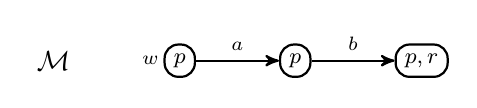
\begin{tikzpicture}[->]
\node [state, label = {[label-state]left:$w$}] (w1) {$p$};
\node[left = of w1] (m) {$\modults$};
\node [state, right = of w1] (w2) {$p$};
\node [state, right = of w2] (w3) {$p,r$};

\path (w1) edge node [label-edge, above] {$a$} (w2)
        (w2) edge node [label-edge, above] {$b$} (w3);
\end{tikzpicture}
\end{tabular}
\begin{picture}(90,0)
\put(20,0){$\Unc(i) = \left\{
    \begin{array}{c}
        \{ab, a\}, \{\epsilon\}
    \end{array}
    \right\}$}
\end{picture} 
%
%  \begin{tabular}{c}
%  \begin{tikzpicture}[node distance = .5em and 2.5em]
%    \draw (0,0) rectangle (1.5cm,1.7cm);
%    \draw (.3cm,.3cm) rectangle (1.2cm,.7cm) node [pos = 0.5] {$a \ \ b \ \ \epsilon$};
%    \draw (.5cm,1.1cm) rectangle (.9cm,1.5cm) node [pos = 0.5] {$ab$};
%  \end{tikzpicture}
%  \end{tabular}
%\end{tabular}
\end{center}
Note that $\modults,w\not\models\khi(p,r)$.
The set $\set{ab,a}$ is not executable at every $p$-state, it is only executable at $w$.
On the other hand, $\set{\epsilon}$ is executable everywhere, but does not lead always to $r$-states.
Moreover, $\modults,w\not\models\learn_i(p,r)$.
The set $\set{\epsilon}$ cannot be refined, and no refinement of $\set{ab,a}$ does the work.
Therefore, agent $i$ cannot learn how to make $r$ true when $p$ holds.

For \Cref{itm:learnboth} consider $\modults'$ as in~\Cref{prop:expref}.
As said, $\modults',w'\not\models\khi(p,q)$.
%again $\modults$ above. %As said, $\modults,w\not\models\kh(p,r)$.
However, there is a way to learn how to achieve $q$ given $p$: it is possible to split the set $\set{a,b}$ into $\set{a}$ and $\set{b}$; hence, $\modults',w'\models \learn_i(p,q)$ (witness $\set{a}$) but also $\modults',w'\models\learn_i(p,\neg q)$ (witness $\set{b}$).
\end{proof}

\Crefitem{itm:nolearnable} shows how, in certain scenarios, there is
no room for learning. For instance, there might be no way to learn how
to cure a disease, if there is no doctor
available or no vaccine has been developed yet. \Crefitem{itm:learnboth} shows how the agent might be able
to learn not only how to make a formula true under a given condition,
but, at the same time, how to make the same formula false under the same condition.

\medskip

Let us go back to analyzing the properties of the logic $\AReflogic$, and their impact in obtaining complete axiomatizations. First, we enumerate some properties that can be expressed in the logic. In particular, the modality $\arefdiam$ is normal and serial, satisfies natural properties 
of Monotonicity and Weakening, but fails for dynamic versions of axioms 4 and 5 (usually known as \emph{positive} and \emph{negative introspection}). 

\medskip 

\begin{proposition}\label{prop:aref-normal-serial}
It follows from the semantics (\Cref{def:sem:aref}) that:
\begin{enumerate}
\item $\models \arefbox(\varphi \ra \psi) \ra (\arefbox\varphi \ra
\arefbox\psi)$.
\item If $\models \varphi$, then $\models \arefbox\varphi$.
\item $\models \arefbox\varphi \ra \arefdiam\varphi$.
%\end{enumerate}
%\end{proposition}

%\begin{proof}
%Let $\modults = \tup{\W,\R,\Unc,\V}$ and $w \in \W$:
%\begin{enumerate}
%\item Suppose $\modults,w \models \arefbox(\varphi \ra \psi)$ and $\modults,w \models \arefbox\varphi$ and let $\plan_1,\plan_2 \in \ACT^*$.
%We have that $\modults,w \models \refbox{\plan_1}{\plan_2}(\varphi \ra \psi)$ and $\modults,w \models \refbox{\plan_1}{\plan_2}\varphi$.
%Using \Cref{itm:distref} from \Cref{prop:ref-normal-serial}, $\modults,w \models \refbox{\plan_1}{\plan_2}\psi$.
%Thus, $\modults,w \models \arefbox\psi$.
%\item Suppose $\models \varphi$ and let $\plan_1,\plan_2 \in \ACT^*$.
%Using \Cref{itm:necessitationref} from \Cref{prop:ref-normal-serial}, $\models \refbox{\plan_1}{\plan_2}\varphi$.
%Thus, $\models \arefbox\varphi$.
%\item Suppose $\modults,w \models \arefbox\varphi$.
%Then, for all $\plan_1,\plan_2 \in \ACT^*$, $\modults,w \models \refbox{\plan_1}{\plan_2}\varphi$.
%Since $\ACT$ is not empty, we choose $\alpha_1, \alpha_2 \in \ACT^*$, and we have that $\modults,w \models \refbox{\alpha_1}{\alpha_2}\varphi$.
%Using \Cref{itm:serialityref} from \Cref{prop:ref-normal-serial}, $\modults,w \models \refdiam{\alpha_1}{\alpha_2}\varphi$.
%Thus, $\modults,w \models \arefdiam\varphi$.
%\end{enumerate}
%\end{proof}

%\begin{proposition}\label{prop:aref-mon-weak-intr}
%Let $\varphi,\psi$ be arbitrary $\Reflogic$-formulas.
%\begin{enumerate}
\item $\models \arefdiam \varphi \ra \arefdiam (\varphi \vee \psi)$ and $\models \arefbox \varphi \ra \arefbox (\varphi \vee \psi)$ (Monotonicity).
\item $\models \arefdiam (\varphi \wedge \psi) \ra \arefdiam \varphi$ and $\models \arefbox (\varphi \wedge \psi) \ra \arefbox \varphi$ (Weakening).
\item $\not\models \arefbox \varphi \ra \arefbox\arefbox \varphi$ (axiom 4). % (Positive Introspection).
\item $\not\models \neg\arefbox \varphi \ra \arefbox\neg\arefbox \varphi$ (axiom 5). % (Negative Introspection).
\end{enumerate}
\end{proposition}

\begin{proof}
%\begin{enumerate}
% \item Suppose $\modults,w \models \arefbox(\varphi \ra \psi)$ and $\modults,w \models \arefbox\varphi$ and let $\plan_1,\plan_2 \in \ACT^*$.
% We have that $\modults,w \models \refbox{\plan_1}{\plan_2}(\varphi \ra \psi)$ and $\modults,w \models \refbox{\plan_1}{\plan_2}\varphi$.
% Using \Cref{itm:distref} from \Cref{prop:ref-normal-serial}, $\modults,w \models \refbox{\plan_1}{\plan_2}\psi$.
% Thus, $\modults,w \models \arefbox\psi$.
% \item Suppose $\models \varphi$ and let $\plan_1,\plan_2 \in \ACT^*$.
% Using \Cref{itm:necessitationref} from \Cref{prop:ref-normal-serial}, $\models \refbox{\plan_1}{\plan_2}\varphi$.
% Thus, $\models \arefbox\varphi$.
% \item Suppose $\modults,w \models \arefbox\varphi$.
% Then, for all $\plan_1,\plan_2 \in \ACT^*$, $\modults,w \models \refbox{\plan_1}{\plan_2}\varphi$.
% Since $\ACT$ is not empty, we choose $\alpha_1, \alpha_2 \in \ACT^*$, and we have that $\modults,w \models \refbox{\alpha_1}{\alpha_2}\varphi$.
% Using \Cref{itm:serialityref} from \Cref{prop:ref-normal-serial}, $\modults,w \models \refdiam{\alpha_1}{\alpha_2}\varphi$.
% Thus, $\modults,w \models \arefdiam\varphi$.
% \end{enumerate}
Items 1 to 3 follows as $\arefdiam$ is a generalization of $\refdiam{\plan_1}{\plan_2}$ from the previous section. 
It is also easy to see that Monotonicity and Weakening are direct. For axiom~4, let us consider the model $\modults = \tup{\W,\R,\Unc,\V}$ depicted below, with $\Unc(i)\in\Unc$ be such that $\Unc(i):=\set{\set{a,b,c}}$.
\begin{center}
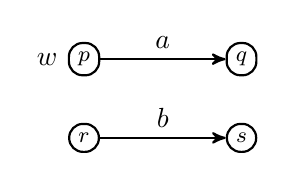
\begin{tikzpicture}[->, grow' = right, level/.style={sibling distance = 3em/#1}, level distance = 3.5em]
\node[state] at (0,2) (p) [label=left:$w$]{$p$};
\node[state] at (2,2) (q) {$q$};
\draw[] (p) node at (1,2) [above] {$a$} -- (q);

\node[state] at (0,1) (r) {$r$};
\node[state] at (2,1) (s) {$s$};
\draw[] (r) node at (1,1) [above] {$b$} -- (s);
\end{tikzpicture}
\end{center}

On the one hand, one can easily check that $\modults,w\models\arefbox\neg(\kh(p,q) \wedge \kh(r,s))$. On the other hand, we have that $\modults,w\models\refdiam{a}{b}\refdiam{b}{c} (\kh(p,q) \wedge \kh(r,s))$. Hence, we get $\modults,w\models\arefdiam\arefdiam(\kh(p,q) \wedge \kh(r,s))$.

For axiom~5, notice that $\modults,w \models \neg\arefbox \kh(p,q)$ but $\modults,w \models \neg\arefbox\neg\arefbox \kh(p,q)$, since $\modults,w \models \refdiam{a}{b}\arefbox \kh(p,q)$.
\end{proof}

Similarly, this modality preserves knowledge and can generate new one for propositional formulas.

\medskip

\begin{proposition}\label{prop:aref-preserves-gains}
Let $\psi,\varphi$ be propositional formulas. Then, 
\begin{enumerate}
\item\label{itm:aref:preservesknowledge} $\models \khi(\psi,\varphi) \ra \arefbox\khi(\psi,\varphi)$.
\item\label{itm:aref:gainsknowledge} If $\psi$ and $\varphi$ are satisfiable, then $\neg\khi(\psi,\varphi) \wedge \arefdiam\khi(\psi,\varphi)$ are satisfiable.
\end{enumerate}
\end{proposition}
\begin{proof}
Similar to \Cref{prop:ref-preserves-gains}.
\end{proof}

By definition, $\models \refdiam{\plan_1}{\plan_2}\varphi \implies \arefdiam\varphi$, but characterizing the exact expressivity relation between the two resulting logics requires further developments.
In particular, given the mismatch between the two languages ($\Reflogic$ is able to talk about specific plans whereas $\AReflogic$ is not), it does not seem trivial to give a translation from one logic to the other.
However, by using the same argument as in \Cref{prop:expref}, it is easy to show the following:

\medskip

\begin{proposition}\label{prop:exparef}
$\AReflogic$ is more expressive than $\KHilogic$.
\end{proposition}

\medskip

Again, we establish that uniform substitution fails in this logic, which in combination with its high expressivity, makes it difficult to axiomatize.

\medskip

\begin{proposition}\label{prop:substitution-aref}
    Uniform substitution fails in $\AReflogic$.
\end{proposition}

\begin{proof}
Similar to~\Cref{prop:substitution-ref}, and taking $p\to\arefdiam p$ as the original valid formula.
\end{proof}

The problem of defining dynamic operators and corresponding axiomatizations will be addressed in the next section. 
We finish the section by stating some expressivity connections between the
dynamic modalities we just discussed.

\medskip

\begin{proposition}\label{prop:explearn}
The following propositions are true:
\begin{enumerate}
\item\label{itm:lhkh} $\LHlogic$ is more expressive than $\KHilogic$.
\item\label{itm:lhref} $\LHlogic$ is not more expressive than $\Reflogic$.
\end{enumerate}
\end{proposition}
\begin{proof}
\Cref{itm:lhkh} is proved as \Cref{prop:expref}: the formula $\learn_i(p,q)$ distinghuishes the two \ultss.
For \Cref{itm:lhref} consider the two \ultss below:
\begin{center}
\begin{tabular}{l@{\qquad\quad}l}
\begin{tabular}{c}
    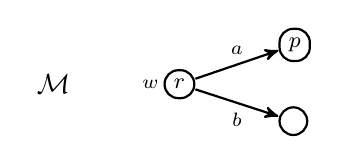
\begin{tikzpicture}[->]
    \node [state, label = {[label-state]left:$w$}] (w1) {$r$};
    \node [state, above right = 0.25em and 3em of w1] (w2) {$p$};
    \node [state, below right = 0.25em and 3em of w1] (w3) {};
    \path (w1) edge node [label-edge, above] {$a$} (w2)
                edge node [label-edge, below] {$b$} (w3);
    \node [ left = of w1] {$\modults$};
    \end{tikzpicture}
\end{tabular}
&
\begin{tabular}{c}
    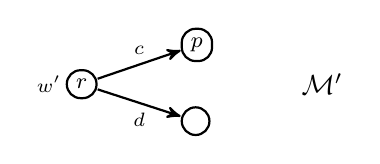
\begin{tikzpicture}[->]
    \node [state, label = {[label-state]left:$w'$}] (w1) {$r$};
    \node [state, above right = 0.25em and 3em of w1] (w2) {$p$};
    \node [state, below right = 0.25em and 3em of w1] (w3) {};
    \path (w1) edge node [label-edge, above] {$c$} (w2)
                edge node [label-edge, below] {$d$} (w3);
    \node [right = 7em of w1] {$\modults'$};
    \end{tikzpicture}
\end{tabular}
\end{tabular} 
\end{center}
For each model, consider respective sets $\Unc(i)=\set{\set{a,b}}$ and $\Unc(i)'=\set{\set{c,d}}$.
Since $\LHlogic$ cannot explicitely talk about plans, $\modults,w$ and $\modults',w'$ are indistinguishable for it.
In $\Reflogic$, $\modults,w\models \dialhepis{a{\not\sim}b}\khi(r,p)$ and $\modults',w'\not\models\dialhepis{a{\not\sim}b}\khi(r,p)$.
\end{proof}



% 
% \begin{proof}
% The formula $\arefdiam\kh(p,q)$ distinguishes the two models in \Cref{prop:expref}. 
% \end{proof}

%  RF: 19/04/2022 Commented as I don't see it is needed
%
% \begin{definition}[Reachability]\label{def:reachability}
% Let $\modults = \tup{\W,\R,\Unc,\V}$ be \ultss. We write  $\splitstr{\Unc}{\Unc'}{}{}$ if there are $\plan_1,\plan_2$ such that  $\splitstr{\Unc}{\Unc'}{\plan_1}{\plan_2}$.
% We say that $\Unc'$ is finitely reachable from $\Unc$ if $\Unc\leadsto^* \Unc'$ (i.e., $\Unc'$ is reached via the reflexive-transitive closure of $\leadsto$). For $\Unc(i),\Unc'_i$,
% $\Unc(i)\leadsto\Unc(i)'$ (resp. $\Unc(i)\leadsto^*\Unc(i)'$) whenever $\Unc\leadsto\Unc'$  (resp., $\Unc\leadsto^*\Unc'$), $\Unc(i)\in\Unc$ and $\Unc(i)'\in\Unc'$.
% \end{definition}

% Note that we always have $\Unc\leadsto\Unc$, by taking since $\plan_1 = \plan_2$.

% \begin{definition}[Submodel]\label{def:submodel}
% Let $\modults = \tup{\W,\R,\Unc,\V}$ and $\modults' = \tup{\W',\R',\Unc',\V'}$ be \ultss, $\modults'$ is a submodel of $\modults$ if $\W' = \W$, $\R' = \R$, $\V' = \V$ and $\Unc\leadsto\Unc'$. 
% We write $\modults' \subseteq \modults$ if $\modults'$ is a submodel of $\modults$.
% Moreover, we denote this model as $\modults_{\Unc'}$.
% \end{definition}
%


% \bigandres{a}

% \begin{definition}
% Let $\modults=\tup{\W,\R,\Unc,\V}$ be an \ults and $U \subseteq \W$.
% $U$ is $\AReflogic$-definable if there is a formula $\varphi \in \AReflogic$ s.t. $U = \truthset{\modults}{\varphi}$.
% $U$ is propositionally-definable if there is a propositional formula $\varphi$ s.t. $U = \truthset{\modults}{\varphi}$.
% \end{definition}

% \begin{claim}
% For any $\modults=\tup{\W,\R,\Unc,\V}$, $\varphi \in \AReflogic$ and $\plan_1,\plan_2 \in \ACT^*$, there is $\Unc' \subseteq 2^{2^{(\ACT^*)}}$ s.t. $\splitstr{\Unc}{\Unc'}{\plan_1}{\plan_2}$ and $\truthset{\modults}{\refdiam{\plan_1}{\plan_2}\varphi} = \truthset{\modults^{\Unc}_{\Unc'}}{\varphi}$.
% \end{claim}
% \begin{proof}
% The case of propositional variables is direct.
% \begin{enumerate}
% \item If $\varphi = \neg\varphi_1$
% \item If $\varphi = \varphi_1 \wedge \varphi_2$
% \item If $\varphi = \khi(\varphi_1,\varphi_2)$, then either $\truthset{\modults}{\refdiam{\plan_1}{\plan_2}\varphi} = \W$ (we choose the witness $\Unc'$) or $\truthset{\modults}{\refdiam{\plan_1}{\plan_2}\varphi} = \emptyset$ (and we choose $\Unc'=\Unc$).
% Either way, the existence of $\Unc'$ is guaranteed.
% \item If $\varphi = \refdiam{\alpha_1}{\alpha_2}\varphi$
% \end{enumerate}
% \end{proof}


% \begin{claim}
% Let $\modults=\tup{\W,\R,\Unc,\V}$ be an \ults and $\varphi \in \AReflogic$ a formula.
% Then there is $\plan_1,\plan_2 \in \ACT^*$ s.t. $\truthset{\modults}{\arefdiam\varphi} = \truthset{\modults}{\refdiam{\plan_1}{\plan_2}\varphi}$.
% \end{claim}

% \begin{claim}
% Let $\modults=\tup{\W,\R,\Unc,\V}$ be an \ults and $\varphi \in \AReflogic$ a formula.
% $\truthset{\modults}{\varphi}$ is propositionally-definable.
% \end{claim}
% \begin{proof}
% The propositional variables and Boolean conectors cases are straightforward.
% Let $\varphi = \khi(\varphi_1,\varphi_2)$, then either $\truthset{\modults}{\varphi}$ is $\emptyset$ $(= \truthset{\modults}{\bot})$ or is $\W$ $(= \truthset{\modults}{\top})$.
% Thus, it is propositionally-definable.
% If $\varphi = \arefdiam \varphi_1$, then $w \in \truthset{\modults}{\varphi}$ iff $\modults,w \models \arefdiam \varphi_1$ iff $\modults,w \models \refdiam{\plan_1}{\plan_2}$

% \end{proof}

% \begin{definition}\label{def:notation-ref} 
% Let $\modults=\tup{\W,\R,\Unc,\V}$ be an \ults.
% For $\strategy \in 2^{\ACT^*}$, $U,T \subseteq \W$,
% \begin{itemize} 
%     \item write $U \ultsExecStrat{\strategy}_{\Unc} T$ {\;\iffdef\;}
%     $U \subseteq \stexec(\strategy)$ and $T = \R_{\strategy}(U)$;
%     \item write $U \ultsExecAgi_{\Unc} T$ {\;\iffdef\;}
%     if there is $\strategy \in \Unc(i)$ such that $\Unc(i)\in\Unc$ and $U \ultsExecStrat{\strategy}_{\Unc} T$.
% \end{itemize}

% Let $Z \subseteq (\W \times 2^{2^{(\ACT^*)}}) \times (\W' \times 2^{2^{(\ACT'^*)}})$ be a relation, then:
% \begin{itemize}
%     \item For $u \in \W$ and $U \subseteq \W$, define:
    
%     \begin{nscenter}
%     \begin{tabular}{@{}c@{}}
%     $Z(u,\Unc,\Unc') := \csetsc{u' \in \W'}{(u,\Unc)Z(u',\Unc')}$;
%     $Z(U,\Unc,\Unc') := \bigcup_{u \in U} Z(u,\Unc,\Unc')$.
%     \end{tabular}
%     \end{nscenter}
    
%     \item For $u' \in \W$ and $U' \subseteq \W'$, define:
    
%     \begin{nscenter}
%     \begin{tabular}{@{\!\!\!\!\!\!\!\!}c@{}}
%     $Z^{-1}(u',\Unc,\Unc') := \csetsc{u \in \W}{(u,\Unc)Z(u',\Unc')}$;
%     $Z^{-1}(U',\Unc,\Unc') := \bigcup_{u' \in U'} Z(u',\Unc,\Unc')$.
%     \end{tabular}
%     \end{nscenter}
%     \end{itemize}
% \end{definition}

% \begin{definition}[$\AReflogic$-bisimulation]\label{def:bisim-aref}
% Let $\modults=\tup{\W,\R,\Unc,\V}$ be an \ults over $\ACT$ and let $\modults'=\tup{\W',\R',\Unc',\V'}$ be an \ults over $\ACT'$.  
% A non-empty $Z \subseteq (\W \times 2^{2^{(\ACT^*)}}) \times (\W' \times 2^{2^{(\ACT'^*)}})$ is called an \emph{$\Reflogic$-bisimulation} between $\modults$ and $\modults'$ if and only if $(w,\Uncother)Z(w',\Uncother')$ implies:
% \begin{description} 
% \item[Atom:] $\V(w)=\V'(w')$.

% \item[$\kh$-Zig:] for any $U \subseteq \W$ that is $\AReflogic$-definable in $\modults_{\Uncother}$, if $U \ultsExecAgi_{\Uncother} T$ for some $T \subseteq \W$, then there is $T' \subseteq \W'$ s.t.
% \begin{ltabular}{l@{\;}l@{\qquad\qquad}l@{\;}l}
% \ITM{i}  & $Z(U,\Uncother,\Uncother') \ultsExecAgi_{\Uncother'} T'$, and &
% \ITM{ii} & $T' \subseteq Z(T,\Uncother,\Uncother')$.
% \end{ltabular}

% \item[$\kh$-Zag:] for any $U' \subseteq \W'$ that is $\AReflogic$-definable in $\modults'_{\Uncother'}$, if $U' \ultsExecAgi_{\Uncother'} T'$ for some $T' \subseteq \W'$, then there is $T \subseteq \W$ s.t.
% \begin{ltabular}{l@{\;}l@{\qquad\qquad}l@{\;}l}
% \ITM{i}  & $Z^{-1}(U',\Uncother,\Uncother') \ultsExecAgi_{\Uncother} T$, and &
% \ITM{ii} & $T \subseteq Z^{-1}(T',\Uncother,\Uncother')$.
% \end{ltabular}

% \item[$\A$-Zig:] for all $u$ in $\W$ there exists $u'$ in $\W'$ such that $(u,\Uncother)Z(u',\Uncother')$.

% \item[$\A$-Zag:] for all $u'$ in $\W'$ there exists$u$ in $\W$ such that $(u,\Uncother)Z(u',\Uncother')$.

% \item[$\arefdiam$-Zig:] for all $\plan_1,\plan_2\in\ACT^*$ and $\Uncter\subseteq 2^{(\ACT^*)}$ such that $\splitstr{\Uncother}{\Uncter}{\plan_1}{\plan_2}$, there are ${\plan'_1,\plan'_2\in\ACT'^*}$ and $\Uncter'\subseteq 2^{(\ACT'^*)}$ such that $\splitstr{\Uncother'}{\Uncter'}{\plan'_1}{\plan'_2}$ and $(w,\Uncter)Z(w',\Uncter')$.

% \item[$\arefdiam$-Zag:] for all $\plan_1',\plan_2'\in\ACT'^*$ and $\Uncter'\subseteq 2^{(\ACT'^*)}$ such that $\splitstr{\Uncother'}{\Uncter'}{\plan_1'}{\plan_2'}$, there are ${\plan_1,\plan_2\in\ACT^*}$ and $\Uncter\subseteq 2^{(\ACT^*)}$ such that $\splitstr{\Uncother}{\Uncter}{\plan_1}{\plan_2}$ and $(w,\Uncter)Z(w',\Uncter')$.
% \end{description}

% We write $\modults,w \bisim_\AReflogic \modults',w'$ when there is an $\AReflogic$-bisimulation $Z$ between $\modults$ and $\modults'$ such that $(w,\Unc)Z(w',\Unc')$.
% \end{definition}

% % \begin{proposition}\label{prop:refbisim-implies-arefbisim}
% % Let $\modults$ and $\modults'$ are \ultss such that $\ACT_{\cap}=\ACT\cap\ACT' \neq \emptyset$ and $\Unc,\Unc' \in 2^{\ACT_{\cap}}$.
% % If ($\modults,w \bisim_\Reflogic \modults',w'$), then ($\modults,w \bisim_\AReflogic \modults',w'$).
% % \end{proposition}
% % \begin{proof}
% % Suppose there are $\plan_1$, $\plan_2$ in $\ACT^*$ and $\overline{\Unc}(0) \in \REACH{\Unc}$ such that $\splitstr{\Unc(0)}{\overline{\Unc}(0)}{\plan_1}{\plan_2}$.
% % Then by \textbf{$\dialhepis{\plan_1{\not\sim}\plan_2}$-Zig}, there are $\plan'_1=\plan_1$, $\plan'_2=\plan_2$ in $\ACT'^*=\ACT^*$ and $\overline{\Unc}'_0 \in \REACH{\Unc'}$ such that $\splitstr{\Unc'_0}{\overline{\Unc}'_0}{\plan'_1}{\plan'_2}$ and $(w,\overline{\Unc}(0))Z(w',\overline{\Unc}'_0)$.
% % With this, we have \textbf{$\arefdiam$-Zig}.
% % With a similar reasoning, we can prove \textbf{$\arefdiam$-Zig}.
% % \end{proof}

% % \begin{definition}[$\AReflogic$-equivalence]\label{def:equiv-aref}
% % The pointed \ultss $\modults, w$ and $\modults', w'$ are \emph{$\AReflogic$-equivalent} (written $\modults, w \modequiv_\AReflogic \modults', w'$) if and only if $\modults, w \models \varphi$ iff $\modults', w' \models \varphi$ for all $\varphi \in \AReflogic$.
% % \end{definition}

% Then we are in position to prove the intended theorem (notice that $\modequiv_\AReflogic$ is defined simply by extending~\Cref{def:equiv-kh} to $\AReflogic$-formulas).

% \begin{theorem}[Invariance for $\AReflogic$]\label{th:arefbisim-to-arefequiv}
% Let $\modults, w$ and $\modults', w'$ be pointed \ultss.
% Then, $\modults,w \bisim_\AReflogic \modults', w' \text{ implies }\modults,w \modequiv_\AReflogic \modults',w'$.
% \end{theorem}
% \begin{proof}
% The proof of $\AReflogic$-equivalence is by structural induction on $\AReflogic$-formulas.
% The goal is to prove that $(u,\Unc(0))Z(u',\Unc(0)')$ (with the induced submodels $\modults_{\Unc(0)} \subseteq \modults$ and $\modults_{\Unc(0)'}' \subseteq \modults'$) implies $\modults_{\Unc(0)},u \modequiv_\Reflogic \modults_{\Unc(0)'}',u'$.
% The cases for atomic propositions and Boolean operators are standard.

% For formulas of the form $\kh(\psi,\varphi)$, we have a similar approach as in Theorem \ref{th:khbisim-to-khequiv}.
% Suppose $u \in \truthset{\modults_{\Unc(0)}}{\kh(\psi,\varphi)}$; then, there is $\strategy \in \Unc(0)$
% s.t. $\truthset{\modults_{\Unc(0)}}{\psi} \ultsExecStrat{\strategy}_{\Unc(0)} T$ and
% $T=\R_{\strategy}(\truthset{\modults_{\Unc(0)}}{\psi}) \subseteq \truthset{\modults_{\Unc(0)}}{\varphi}$.
% First, note how $Z(\truthset{\modults_{\Unc(0)}}{\psi},\Unc(0),\Unc(0)') = \truthset{\modults_{\Unc(0)'}'}{\psi}$.
% Indeed, $(\subseteq)$ if $v' \in Z(\truthset{\modults_{\Unc(0)}}{\psi},\Unc(0),\Unc(0)')$, then there is $v \in \truthset{\modults_{\Unc(0)}}{\psi}$ such that $(v,\Unc(0))Z(v',\Unc(0)')$; thus, from IH we have $v' \in \truthset{\modults_{\Unc(0)'}'}{\psi}$.
% $(\supseteq)$ If $v' \in \truthset{\modults_{\Unc(0)'}'}{\psi}$, by $\A$-Zag there is $v$ with $(v,\Unc(0))Z(v',\Unc(0)')$; thus, from IH we have $v \in \truthset{\modults_{\Unc(0)}}{\psi}$.
% Hence, $v' \in Z(\truthset{\modults_{\Unc(0)}}{\psi},\Unc(0),\Unc(0)')$.

% The set $\truthset{\modults_{\Unc(0)}}{\psi}$ is $\Reflogic$-definable.
% % \textcolor{red}{(we are not sure if it is also propositionally definable; if not, we can redefine bisimulations; from here the proof assumes it is the case) and thus propositionally definable}. \raul{creo que como la modalidad dinamica es global, esto deberia valer de todos modos, pero en el modelo adecuado}
% Thus, there are $\strategy \in \Unc(0)$ and $T \subseteq \W$ such that $\truthset{\modults_{\Unc(0)}}{\psi} \ultsExecStrat{\strategy}_{\Unc(0)} T$, so $\truthset{\modults_{\Unc(0)}}{\psi} \ultsExec_{\Unc(0)} T$.
% Then, from the latter and clause $\kh$-Zig, there is $T' \subseteq \W'$ such that

% \begin{enumerate}
% \item $Z(\truthset{\modults_{\Unc(0)}}{\psi},\Unc(0),\Unc(0)') \ultsExec_{\Unc(0)'} T'$ (so $\truthset{\modults_{\Unc(0)'}'}{\psi} \ultsExec_{\Unc(0)'} T'$, by the result above), and
% \item\label{itm:ii} $T' \subseteq Z(T,\Unc(0),\Unc(0)')$.
% \end{enumerate}

% Now, we know that $T \subseteq \truthset{\modults_{\Unc(0)}}{\varphi}$, that is, $v \in T$ implies $v \in \truthset{\modults_{\Unc(0)}}{\varphi}$.
% But then, by IH, $v \in T$ and $(v,\Unc(0))Z(v',\Unc(0)')$ implies $v' \in \truthset{\modults_{\Unc(0)'}'}{\varphi}$.
% Thus, $Z(T,\Unc(0),\Unc(0)') \subseteq \truthset{\modults_{\Unc(0)'}'}{\varphi}$.
% This, together with \itm{\ref{itm:ii}} from the previous paragraph, yields $T' \subseteq \truthset{\modults_{\Unc(0)'}'}{\varphi}$.
% Thus, we have both $\truthset{\modults_{\Unc(0)'}'}{\psi} \ultsExec_{\Unc(0)'} T'$ (there is an strongly executable strategy which, from $\psi$-worlds, reaches only $T'$-worlds) and $T' \subseteq \truthset{\modults_{\Unc(0)'}'}{\varphi}$ (every $T'$-world satisfies $\varphi$); hence, $u' \in \truthset{\modults_{\Unc(0)}'}{\kh(\psi,\varphi)}$.

% The direction from $u' \in \truthset{\modults_{\Unc(0)'}'}{\kh(\psi,\varphi)}$ to $u \in \truthset{\modults_{\Unc(0)}}{\kh(\psi,\varphi)}$ follows a similar argument, using $\A$-Zig and $\kh$-Zag instead.

% For the case $\arefdiam\varphi$, suppose $\modults_{\Unc(0)},u \models \arefdiam \varphi$.
% Then, there are $\plan_1,\plan_2 \in \ACT^*$ $\modults,w\models\dialhepis{\plan_1{\not\sim}\plan_2}\varphi$.
% That is, there is $\overline{\Unc}(0) \in \REACH{\Unc}$ s.t.
% $\splitstr{\Unc(0)}{\overline{\Unc}(0)}{\plan_1}{\plan_2}$ and
% $\modults^{\Unc(0)}_{\overline{\Unc}(0)} = \modults_{\overline{\Unc}(0)},u \models \varphi$.
% Then, by $\arefdiam$-Zig, there are $\plan'_1,\plan'_2 \in \ACT'^*$ and
% $\overline{\Unc}(0)' \in \REACH{\Unc'}$ such that
% $\splitstr{\Unc(0)'}{\overline{\Unc}(0)'}{\plan'_1}{\plan'_2}$
% and $(u,\overline{\Unc}(0))Z(u',\overline{\Unc}(0)')$.
% By IH, $\modults'_{\overline{\Unc}(0)'} = (\modults')^{\Unc(0)'}_{\overline{\Unc}(0)'},u' \models \varphi$.
% And by the definition of $\dialhepis{\plan'_1{\not\sim}\plan'_2}$,
% $\modults',u' \models \dialhepis{\plan'_1{\not\sim}\plan'_2}\varphi$.
% With this, $\modults_{\Unc'_0},u \models \arefdiam \varphi$.

% The direction from $\modults'_{\Unc(0)'},u' \models \arefdiam \varphi$
% to $\modults_{\Unc(0)},u \models \arefdiam \varphi$ follows a similar
% argument, using $\arefdiam$-Zag instead.
% \end{proof}

% % \begin{proposition}
% % Let $\Unc \in 2^{\ACT}$. If $\Unc$ is finite and every $\strategy \in \Unc$, $\strategy$ is finite, then the set $\REACH{\Unc}$ is finite.
% % \end{proposition}
% % \begin{proof}
% % $\REACH{\Unc}$ is at most $\pow(\bigcup_{\strategy \in \Unc} \strategy)$.
% % Since $\bigcup_{\strategy \in \Unc} \strategy$ is finite, then $\REACH{\Unc}$ it is also finite.
% % \end{proof}

% % \begin{theorem}\label{th:arefequiv-to-arefbisim}
% % Let $\modults, w$ and $\modults', w'$ be pointed \ultss. If $\modults$ and $\modults'$ are
% % finite then $\modults,w \modequiv_\AReflogic \modults', w'$ implies
% % $\modults,w \bisim_\AReflogic \modults', w'$.
% % \end{theorem}

% % \begin{proof}
% % As it happened in \Cref{th:khequiv-to-khbisim}, the restriction to finite models (instead of just ``image finite'') is needed because the universal modality is definable in $\KHilogic$.
% % Take $\modults=\tup{\W,\R,\Unc,\V}$ and $\modults'=\tup{\W',\R',\Unc',\V'}$.
% % The strategy is to show that the relation $\modequiv$ is already a bisimulation.
% % Thus, define $Z := \csetc{(v,\Unc(0),v',\Unc(0)')}{(\W \times \REACH{\Unc}) \times (\W' \times \REACH{\Unc'})}{\modults_{\Unc(0)}, v \modequiv_\AReflogic \modults'_{\Unc(0)'}, v'}$; in order to show that $Z$ satisfies the requirements, take any $(w,\Unc(0),w'\Unc(0)') \in Z$.

% % \begin{itemize}
% % \item \textbf{Atom}. States $w$ and $w'$ coincide in all $\AReflogic$-formulas, and in particular, in all atoms.

% % \item \textbf{$\A$-Zig}. Take $v \in \W$ and suppose, for the sake of a contradiction, that there is no $v' \in \W'$ such that $(v,\Unc(0))Z(v',\Unc(0)')$.
% % Then, from $Z$'s definition, for each $v_i'\in \W' = \set{v'_1,\ldots,v'_n}$ (recall: $\modults'_{\Unc(0)'}$ is finite) there is a $\Reflogic$-formula $\theta_i$ s.t. $\modults_{\Unc(0)},v \models \theta_i$ but $\modults'_{\Unc(0)'},v'_i \not\models \theta_i$.
% % Now take $\theta := \theta_1 \land \cdots \land \theta_n$.
% % Clearly, $\modults_{\Unc(0)'},v \models \theta$; however, $\modults'_{\Unc(0)'},v_i' \not\models \theta$ for each $v_i'\in \W'$, as each one of them makes `its' conjunct $\theta_i$ false.
% % Then, by taking $\E \varphi := \lnot \A \lnot \varphi$ we have $\modults_{\Unc(0)},w \models \E \theta$ but $\modults'_{\Unc(0)'},w' \not\models \E \theta$, contradicting $(w,\Unc(0))Z(w',\Unc(0)')$.

% % \item \textbf{$\A$-Zag}. Analogous to the $\A$-Zig case.

% % \item \textbf{$\kh$-Zig}. Take \textcolor{red}{any propositionally definable set} $\truthset{\modults_{\Unc(0)}}{\psi} \subseteq \W$ (thus, $\psi$ is propositional), and suppose $\truthset{\modults_{\Unc(0)}}{\psi} \ultsExec_{\Unc(0)} T$ for some $T \subseteq \W$.
% % We need to find a $T' \subseteq \W'$ s.t.

% % \begin{enumerate}
% % \item $Z(\truthset{\modults_{\Unc(0)}}{\psi},\Unc(0),\Unc(0)') \ultsExec_{\Unc(0)'} T'$ and
% % \item $T' \subseteq Z(T,\Unc(0),\Unc(0)')$.
% % \end{enumerate}

% % First, note that $\truthset{\modults'_{\Unc(0)'}}{\psi} = Z(\truthset{\modults_{\Unc(0)}}{\psi})$. For $\boldsymbol{(\supseteq)}$, suppose $u' \in Z(\truthset{\modults_{\Unc(0)}}{\psi})$.
% % Then, there is $u \in \truthset{\modults_{\Unc(0)}}{\psi}$ such that $(u,\Unc(0))Z(u',\Unc(0)')$, and therefore, from $Z$'s definition, $u' \in \truthset{\modults'_{\Unc(0)'}}{\psi}$.
% % For $\boldsymbol{(\subseteq)}$, suppose $u' \in \truthset{\modults'_{\Unc(0)'}}{\psi}$.
% % From $\A$-Zag, there is $u \in \W$ such that $(u,\Unc(0))Z(u',\Unc(0)')$; then, from $Z$'s definition, $u \in \truthset{\modults_{\Unc(0)}}{\psi}$ so $u' \in Z(\truthset{\modults_{\Unc(0)}}{\psi})$.

% % Thus, we are actually looking for a $T' \subseteq \W'$ such that

% % \begin{enumerate}
% % \item $\truthset{\modults'_{\Unc(0)'}}{\psi} \ultsExec_{\Unc(0)'} T'$ and
% % \item $T' \subseteq Z(T,\Unc(0),\Unc(0)')$
% % \end{enumerate}

% % Consider the two alternatives.
% % \begin{enumerate}
% % \item If $\truthset{\modults_{\Unc(0)}}{\psi} = \emptyset$, then $\truthset{\modults'_{\Unc(0)'}}{\psi} = Z(\truthset{\modults_{\Unc(0)}}{\psi}) = \emptyset$ and hence taking $T' = \emptyset$ does the job: clearly,
% % \begin{enumerate}
% % \item $\emptyset \ultsExec_{\Unc(0)'} \emptyset$ (as $\Unc(0)' \neq \emptyset$) and
% % \item $\emptyset \subseteq Z(T,\Unc(0),\Unc(0)')$.
% % \end{enumerate}

% % \item Otherwise, $\truthset{\modults_{\Unc(0)}}{\psi} \neq \emptyset$ and $T \neq \emptyset$.
% % Then, from $\A$-Zig it follows that $Z(\truthset{\modults_{\Unc(0)}}{\psi}) = \truthset{\modults'_{\Unc(0)'}}{\psi} \neq \emptyset$.
% % In order to show that there is a $T' \subseteq \W'$ satisfying both {\itshape \bfseries (i)} and {\itshape \bfseries (ii)}, the argument is by contradiction.
% % Thus, suppose there is no $T'$ with the given requirements: each $T' \subseteq \W'$ satisfying $\truthset{\modults'_{\Unc(0)'}}{\psi} \ultsExec_{\Unc(0)'} T'$ is such that $T' \not\subseteq Z(T)$.
% % In other words, for every $T' \subseteq \W'$ satisfying $\truthset{\modults'_{\Unc(0)'}}{\psi} \ultsExec_{\Unc(0)'} T'$ there is a $v'_{T'} \in T'$ such that there is no $v \in T$ with $(v,\Unc(0))Z(v'_{T'},\Unc(0)')$.
% % Due to the definition of $Z$, this means that for each $v \in T$ there is a formula $\theta^v_{T'}$ such that $\modults_{\Unc(0)}, v \models \theta^v_{T'}$ but $\modults'_{\Unc(0)'}, v'_{T'} \not\models\theta^v_{T'}$.
% % Since the models are finite, one can define both

% % \begin{nscenter}
% % \renewcommand{\arraystretch}{1.8}
% % \begin{tabular}{ccc}
% % $\displaystyle \theta_{T'} := \bigvee_{v \in T} \theta^v_{T'}$ & and &
% % $\displaystyle \theta :=
% % \bigwedge_{\csetsc{T' \subseteq \W'}{\truthset{\modults'_{\Unc(0)'}}{\psi} \ultsExec_{\Unc(0)'} T'}} \theta_{T'}$.
% % \end{tabular}
% % \renewcommand{\arraystretch}{1}
% % \end{nscenter}

% % Since $T \neq \emptyset$, $\theta_{T'}$ does not collapse to $\bot$.
% % However, $\theta$ can collapse to $\top$ since $\csetsc{T' \subseteq \W'}{\truthset{\modults'_{\Unc(0)}}{\psi} \ultsExec_{\Unc(0)'} T'}$ might be empty.
% % This is what creates the following two cases.

% % \begin{itemize}
% % \item Suppose $\csetsc{T' \subseteq \W'}{\truthset{\modults'_{\Unc(0)}}{\psi} \ultsExec_{\Unc(0)'} T'} = \emptyset$.
% % Then, consider the formula $\kh(\psi,\top)$.
% % Since $\truthset{\modults_{\Unc(0)}}{\psi} \ultsExec_{\Unc(0)'} T$ and $T \subseteq \W = \truthset{\modults_{\Unc(0)}}{\top}$, it follows that $\modults_{\Unc(0)},w \models \kh(\psi, \top)$.
% % However, $\modults'_{\Unc(0)'},w' \not\models \kh(\psi, \top)$ as, according to this case, there is no $T' \subseteq \W'$ with $\truthset{\modults'_{\Unc(0)'}}{\psi} \ultsExec_{\Unc(0)'} T'$.
% % This contradicts the $\AReflogic$-equivalence of $w$ and $w'$.

% % \item Suppose $\csetsc{T' \subseteq \W'}{\truthset{\modults'_{\Unc(0)}}{\psi} \ultsExec_{\Unc(0)'} T'} \neq \emptyset$.
% % Then, $\theta$ does not collapse to $\top$.
% % Note how $\modults_{\Unc(0)}, v \models \theta$ for all $v \in T$, as every such $v$ satisfies its `own' disjunct $\theta^v_{T'}$ in each conjunct $\theta_{T'}$.
% % Hence, from $\truthset{\modults_{\Unc(0)}}{\psi} \ultsExec_{\Unc(0)} T$ it follows that $\modults_{\Unc(0)},w \models \kh(\psi, \theta)$.
% % However, for every $T'$ satisfying  $\truthset{\modults'_{\Unc(0)'}}{\psi} \ultsExec_{\Unc(0)'} T'$ the state $v'_{T'}$ that cannot be matched with any state $v \in T$ makes all disjuncts $\theta^v_{T'}$ in $\theta_{T'}$ false, thus falsifying $\theta_{T'}$ and therefore falsifying $\theta$ too.
% % In other words, every $T' \subseteq \W'$ with $\truthset{\modults'_{\Unc(0)'}}{\psi} \ultsExec_{\Unc(0)'} T'$ contains a state $t'_{T'}$ with $\modults'_{\Unc(0)'}, t'_{T'} \not\models \theta$, that is, $\truthset{\modults'}{\psi} \ultsExec_{\Unc(0)'} T'$ implies $T' \not\subseteq \truthset{\modults_{\Unc(0)}}{\theta}$.
% % Hence, using again the fact that $\kh$-formulas are global, $\modults'_{\Unc(0)'},w' \not\models \kh(\psi, \theta)$, contradicting the $\AReflogic$-equivalence of $w$ and $w'$.
% % \end{itemize}

% % \end{enumerate}

% % \item \textbf{$\kh$-Zag}. Analogous to the $\kh$-Zig case.

% % \item \textbf{$\arefdiam$-Zig}.
% % Let $\plan_1$, $\plan_2$ in $\ACT^*$ and $\overline{\Unc}(0)$ in $\REACH{\Unc}$ such that $\splitstr{\Unc(0)}{\overline{\Unc}(0)}{\plan_1}{\plan_2}$.
% % Suppose there are no $\plan'_1$, $\plan'_2$ in $\ACT'^*$ and $\overline{\Unc}'_0$ in $\REACH{\Unc'}$ such that $\splitstr{\Unc'_0}{\overline{\Unc}'_0}{\plan_1}{\plan_2}$ and $(w,\overline{\Unc}(0))Z(w',\overline{\Unc}'_0)$.
% % That is, for all $\plan'_1$, $\plan'_2$ in $\ACT'^*$ and $\overline{\Unc}'_0 \in \REACH{\Unc'}$ such that $\splitstr{\Unc'_0}{\overline{\Unc}'_0}{\plan_1}{\plan_2}$, $(w,\overline{\Unc}(0),w',\overline{\Unc}'_0) \not\in Z$. By definition of $Z$, let $\theta_{\overline{\Unc}'_0}$ such that $\modults'_{\overline{\Unc}'_0}, w \models \theta_{\overline{\Unc}'_0}$ but $\modults_{\overline{\Unc}(0)}, w \not\models \theta_{\overline{\Unc}'_0}$.
% % Let $\theta$ the finite disjuction of all $\theta_{\overline{\Unc}'_0}$ (recall: $\REACH{S'}$ is finite), then $\modults'_{\Unc'_0}, w \models \arefbox \theta$ but $\modults_{\Unc(0)}, w \not\models \arefbox \theta$ with $\overline{\Unc}(0)$ as the witness.

% % \item \textbf{$\arefdiam$-Zag}. Analogous to the $\arefdiam$-Zig case.

% % \end{itemize}
% % \end{proof}

% % \begin{theorem}\label{aref-not-in-ref}
% % $\AReflogic \not\leq \Reflogic$ (i.e., $\Reflogic$ is not more expressive than $\AReflogic$).
% % \end{theorem}
% % \begin{proof}
% % Sketch idea: For a certain $\ACT$, $\arefdiam \varphi$ if and only iff $\bigvee_{\plan_1,\plan_2 \in \ACT^*} \dialhepis{\plan_1{\not\sim}\plan_2}\varphi$.
% % There should be no finite formula in $\Reflogic$ $\psi$ such that $\bigvee_{\plan_1,\plan_2 \in \ACT^*} \dialhepis{\plan_1{\not\sim}\plan_2}\varphi$ if and only iff $\psi$.
% % \end{proof}
% % 
% % \begin{theorem}\label{aref-not-in-ref}
% % $\Reflogic \not\leq \AReflogic$ (i.e., $\AReflogic$ is not more expressive than $\Reflogic$).
% % \end{theorem}
% % \begin{proof}
% % Sketch idea: Find $\modults$ and $\modults'$ \ultss such that $\ACT_{\cap}=\ACT\cap\ACT' \neq \emptyset$ and $\Unc,\Unc' \in 2^{\ACT_{\cap}}$ such that ($\modults,w \bisim_\AReflogic \modults',w'$) but ($\modults,w \not\modequiv_\Reflogic \modults',w'$).
% % With this, ($\modults,w \modequiv_\AReflogic \modults',w'$).
% % Then pick a certain formula of $\Reflogic$.
% % \end{proof}
% % 
% % \begin{corollary}
% % $\Reflogic$ and $\AReflogic$ are incomparable.
% % \end{corollary}


% \subsection{Goal directed learning how}
% \label{sec:learning}
% One might notice that knowing how operators are \emph{goal-directed}: the agent looks for a suitable course of action that makes her achieve a certain state.
It is possible to define an operator that, when possible, \emph{guarantees} that the agent \emph{learns how} to achieve a goal.
This action can be understood as a goal-directed learning how: it looks for a way to split \emph{some} existing set of plans $\plans$ in such a way that the agent knows how to achieve $\varphi$ given $\psi$. \raul{I am wondering whether introduce a new modality of simply stating only properties of learnability.}

Let $\LHlogic$ (for ``learning how'') be $\KHilogic$ extended with the dynamic modality
\[
\lh{\psi}{\varphi}_i\chi := \arefdiam(\khi(\psi,\varphi) \wedge\chi),
\]
(and its `dual' $[\psi,\varphi]_i\chi := \neg\lh{\psi}{\varphi}_i\neg\chi$).
Moreover, we define $\learn_i(\psi,\varphi) := \lh{\psi}{\varphi}_i\top$ an abbreviation for \emph{``the agent $i$ can learn how to make $\varphi$ true in the presence of $\psi$''}.
Notice that $\LHlogic$ is a syntactic fragment of $\AReflogic$.

The new dynamic modality is a ternary modality expressing that the agent is able to learn how to achieve $\varphi$ given $\psi$, and that after this learning operation takes place, $\chi$ holds.
%However, as we will see below, it can be seen as a unary modality similarly to public announcements or action models.
The modality $\learn_i$ is a test of what is learnable by the agent~$i$.
Note that $\LHlogic$ is a syntactic fragment of $\AReflogic$ y thus reducible to the latter.
However, $\AReflogic$ is indeed reducible to $\LHlogic$ and thus equivalent.

\medskip

\begin{proposition}\label{prop:lhequivaref}
$\LHlogic \equiv \AReflogic$
\end{proposition}
\begin{proof}
As $\LHlogic$ is a syntactic fragment of $\AReflogic$, then $\LHlogic \preceq \AReflogic$.
Por the other direction, we have the following translation function $T: \AReflogic \to \LHlogic$ defined inductively as follows:
\begin{itemize}
\item $T(p) = p$,
\item $T(\neg \varphi_1) = \neg T(\varphi_1)$,
\item $T(\varphi_1 \vee \varphi_2) = T(\varphi_1) \vee T(\varphi_2)$,
\item $T(\khi(\varphi_1, \varphi_2)) = \khi(T(\varphi_1), T(\varphi_2))$, and
\item $T(\arefdiam \varphi_1) = \arefdiam (\khi(\bot,\bot) \wedge T(\varphi_1)) = \lh{\bot}{\bot}_i T(\varphi_1)$.
\end{itemize}

The goal is to prove by induction that for all $\varphi$ $\AReflogic$-formula, there exists $\varphi' = T(\varphi)$ s.t. for all \ults $\modults$ and $w \in \D{\modults}$, we have that $\modults,w \models \varphi$ iff $\modults,w \models T(\varphi)$.
With this, $\AReflogic \preceq \LHlogic$. The first four cases hold using the definition of $\models$ and inductive hypothesis. Therefore, we will focus on the $\arefdiam$ case.
Let $\modults = \tup{\W,\R,\Unc,\V}$ an \ults y $w \in \D{\modults}$, $\modults,w \models \arefdiam \varphi_1$ iff there exist $\plan_1,\plan_2 \in \ACT^*$ s.t. $\modults,w \models \refdiam{\plan_1}{\plan_2}\varphi_1$.
This is equivalent to that there exist $\plan_1,\plan_2 \in \ACT^*$ and $\Unc'$ s.t. $\splitstr{\Unc}{\Unc'}{\plan_1}{\plan_2}$ y $\modults^{\Unc}_{\Unc'},w \models \varphi_1$.
By inductive hypothesis, $\modults^{\Unc}_{\Unc'},w \models T(\varphi_1)$.
As $\khi(\bot,\bot)$ is a valid formula (by definition of $\Unc(i) \neq \emptyset$), it holds true at every model.
Then, $\modults^{\Unc}_{\Unc'},w \models \khi(\bot, \bot) \wedge T(\varphi_1)$ and using the definitions of $\models$ and $T$, it is equivalent to $\modults,w \models T(\arefdiam \varphi_1)$.
Hence, $\AReflogic \preceq \LHlogic$ and $\AReflogic \equiv \LHlogic$.
\end{proof}

Thus, each of these logics can describe the concept of learning how.
Getting back to the dynamic modalities, the following proposition illustrates some properties.

\medskip

\begin{proposition}\label{prop:nolearn}
It follows from the semantics that:
\begin{enumerate}
\item\label{itm:nolearnable} $\not\models\learn_i(\varphi,\psi)$; %and $\not\models\lh{\psi}{\varphi}\kh(\psi,\varphi)$;
\item\label{itm:learnboth} $\learn_i(\varphi,\psi) \wedge \learn_i(\varphi,\neg\psi)$ is satisfiable.
%$\lh{\varphi}{\psi}\kh(\varphi,\psi)\wedge\lh{\varphi}{\psi}\kh(\varphi,\neg\psi)$ is satisfiable.
\end{enumerate}
\end{proposition}

\begin{proof}
\Cref{itm:nolearnable} shows that not everything is learnable by an agent.
%The properties of the underlying LTS
The (un)avail\-abil\-i\-ty of certain actions in an \ults restricts
what can be learnt.  Consider the following single-agent \ults $\modults$, with
the set $\Unc(i)$ shown on the right.
\begin{center}
\begin{tabular}{c}
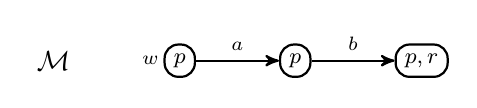
\begin{tikzpicture}[->]
\node [state, label = {[label-state]left:$w$}] (w1) {$p$};
\node[left = of w1] (m) {$\modults$};
\node [state, right = of w1] (w2) {$p$};
\node [state, right = of w2] (w3) {$p,r$};

\path (w1) edge node [label-edge, above] {$a$} (w2)
        (w2) edge node [label-edge, above] {$b$} (w3);
\end{tikzpicture}
\end{tabular}
\begin{picture}(90,0)
\put(20,0){$\Unc(i) = \left\{
    \begin{array}{c}
        \set{ab, a}, \set{\epsilon}
    \end{array}
    \right\}$}
\end{picture} 
%
%  \begin{tabular}{c}
%  \begin{tikzpicture}[node distance = .5em and 2.5em]
%    \draw (0,0) rectangle (1.5cm,1.7cm);
%    \draw (.3cm,.3cm) rectangle (1.2cm,.7cm) node [pos = 0.5] {$a \ \ b \ \ \epsilon$};
%    \draw (.5cm,1.1cm) rectangle (.9cm,1.5cm) node [pos = 0.5] {$ab$};
%  \end{tikzpicture}
%  \end{tabular}
%\end{tabular}
\end{center}
Note that $\modults,w\not\models\khi(p,r)$.
The set $\set{ab,a}$ is not executable at every $p$-state, it is only executable at $w$.
On the other hand, $\set{\epsilon}$ is executable everywhere, but does not lead always to $r$-states.
Moreover, $\modults,w\not\models\learn_i(p,r)$.
The set $\set{\epsilon}$ cannot be refined, and no refinement of $\set{ab,a}$ does the work.
Therefore, agent $i$ cannot learn how to make $r$ true when $p$ holds.

For \Cref{itm:learnboth} consider $\modults'$ as in~\Cref{prop:expref}.
As said, $\modults',w'\not\models\khi(p,q)$.
%again $\modults$ above. %As said, $\modults,w\not\models\kh(p,r)$.
However, there is a way to learn how to achieve $q$ given $p$: it is possible to split the set $\set{a,b}$ into $\set{a}$ and $\set{b}$; hence, $\modults',w'\models \learn_i(p,q)$ (witness $\set{a}$) but also $\modults',w'\models\learn_i(p,\neg q)$ (witness $\set{b}$).
\end{proof}

\Crefitem{itm:nolearnable} shows how, in certain scenarios, there is
no room for learning. For instance, there might be no way to learn how
to cure a disease, if there is no doctor
available or no vaccine has been developed yet. \Crefitem{itm:learnboth} shows how the agent might be able
to learn not only how to make a formula true under a given condition,
but, at the same time, how to make the same formula false under the same condition.

Once more, $[\chi,\psi]$ (seen as a unary modality) is a \emph{normal modality}:
% the distributivity axiom {\sf DISTLh} and the
% necessitation rule {\sf NECLh} are valid over arbitrary \ults{s}:

\medskip

\begin{proposition}\label{prop:lhgoal-normal}
The modality $[\chi,\psi]$ is normal:
\begin{enumerate}
\item\label{itm:distaxiom} $\models[\chi,\psi](\theta \ra \varphi) \ra ([\chi,\psi]\theta \ra [\chi,\psi]\varphi)$.
\item\label{itm:necessitation} If $\models\varphi$, then $\models{[\chi,\psi]\varphi}$.
\end{enumerate}
\end{proposition}

\medskip

%%
%% MARCH 5, 2020: INTERESTING FOR LONG VERSION, BUT REMOVE IT FOR SAVING SPACE
%%
% \begin{proposition}\label{prop:nosubs}
%   The following properties follow:
%   \begin{enumerate}
%     \item\label{itm:nocompkhlh} $\not\models\kh(\chi,\theta)\wedge\lh{\theta}{\psi}\varphi \ra \lh{\chi}{\psi}\varphi$;
%     \item\label{itm:nocomplhlh} $\not\models\lh{\chi}{\theta}\lh{\theta}{\psi}\varphi \ra \lh{\chi}{\psi}\varphi$;
%     \item\label{itm:khpres} $\models\kh(\chi,\psi) \wedge \varphi \ra \lh{\chi}{\psi}\varphi$.
%   \end{enumerate}
%  \end{proposition}

% Notice that if $\kh(\chi,\psi)$ holds, there is some strategy $\plans$
% leading from $\chi$-states to $\psi$-states. By taking the refinement
% $\set{\plans,\emptyset}$ of $\plans$, we satisfy the required
% semantic condition for the dynamic modality, without changing the knowledge
% of the agent.

We finish the section by stating some expressivity connections between the
dynamic modalities we just discussed.

\medskip

\begin{proposition}\label{prop:explearn}
The following propositions are true:
\begin{enumerate}
\item\label{itm:lhkh} $\LHlogic$ is more expressive than $\KHilogic$.
\item\label{itm:lhref} $\LHlogic$ is not more expressive than $\Reflogic$.
\end{enumerate}
\end{proposition}
\begin{proof}
\Cref{itm:lhkh} is proved as \Cref{prop:expref}: the formula $\learn_i(p,q)$ distinghuishes the two \ultss.
For \Cref{itm:lhref} consider the two \ultss below:
\begin{center}
\begin{tabular}{l@{\qquad\quad}l}
\begin{tabular}{c}
    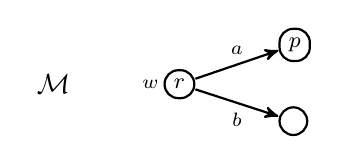
\begin{tikzpicture}[->]
    \node [state, label = {[label-state]left:$w$}] (w1) {$r$};
    \node [state, above right = 0.25em and 3em of w1] (w2) {$p$};
    \node [state, below right = 0.25em and 3em of w1] (w3) {};
    \path (w1) edge node [label-edge, above] {$a$} (w2)
                edge node [label-edge, below] {$b$} (w3);
    \node [ left = of w1] {$\modults$};
    \end{tikzpicture}
\end{tabular}
&
\begin{tabular}{c}
    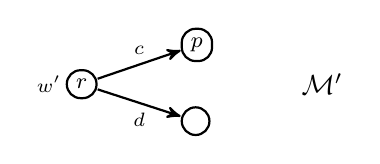
\begin{tikzpicture}[->]
    \node [state, label = {[label-state]left:$w'$}] (w1) {$r$};
    \node [state, above right = 0.25em and 3em of w1] (w2) {$p$};
    \node [state, below right = 0.25em and 3em of w1] (w3) {};
    \path (w1) edge node [label-edge, above] {$c$} (w2)
                edge node [label-edge, below] {$d$} (w3);
    \node [right = 7em of w1] {$\modults'$};
    \end{tikzpicture}
\end{tabular}
\end{tabular} 
\end{center}
For each model, consider respective sets $\Unc(i)=\set{\set{a,b}}$ and $\Unc(i)'=\set{\set{c,d}}$.
Since $\LHlogic$ cannot explicitely talk about plans, $\modults,w$ and $\modults',w'$ are indistinguishable for it.
In $\Reflogic$, $\modults,w\models \dialhepis{a{\not\sim}b}\khi(r,p)$ and $\modults',w'\not\models\dialhepis{a{\not\sim}b}\khi(r,p)$.
\end{proof}


\section{Epistemic updates: extending the basic language}
\label{sec:extension}

A recurring issue when defining both ontic and epistemic updates is the lack of reduction axioms over a general class of models. The reason for this is that the expressivity of the basic language is not enough to describe the effects produced by the update modalities. This makes sense, as the modality $\kh_i$ is very simple, and cannot express properties about explicit courses of action. 
%
%Thus, we managed to define updates for instance for which completeness can be obtained only over a restricted class of models. Moreover, it seems hard to obtain completeness by using a different method. It is well-known that dynamic modalities suffer the lack of desirable properties (from an axiomatizability perspective) such as uniform substitution (see, e.g.,~\cite{HoHoIc11,ArecesFH15}). Naturally, this is also the case for some of our modalities. 
%
% A persistent constraint about the definition of the previous ontic and epistemic operators is that:
% (1) the knowing how modality cannot express explicitly about the plan that meets the requirements to be a proper course of action; and
% (2) to achieve completeness, it is compulsory to limit the scope of the models we are considering.
%
This section explores a different alternative: enrich the underlying static language $\KHilogic$ with a modality to explicitly talk about the actions (or courses of actions) that the agents can take. This modality is simply the basic modal logic operator $\mlbox{a}$ (with $a\in\ACT$). 
%Thus, by extending the axiom system presented in~\Cref{tab:khiaxiom}, we are able to prove that the new logic is sound and complete.
%Moreover, with a similar definition of filtrations used in \cite{mlbook}, we prove that this logic is decidable. \raul{to be checked} 
%Once this has been done, we will be in position to introduce a series of dynamic epistemic operators. The gain of this new approach is that, due to the expressivity added in the underlying static language, we are able to provide reduction axioms for axiomatizing the dynamic modalities over the class of all models.
%Concretely, the meaning of these operators simply reflect situations in which it is announced to all agents (or a group of them) that a plan $\plan$ is distinguishable from every other.

\subsection{The extended basic logic}

We start by introducing the syntax and semantics of the logic $\KHiMLlogic$,  an extension of $\KHilogic$ with the standard $\mlbox{a}$ modality (see e.g.,~\cite{HML,mlbook}).

\medskip

\begin{definition}\label{def:khimlsyntax}
Formulas of the language $\KHiMLlogic$ are defined by the following grammar
\begin{spcenter}
$\varphi ::= p \mid \neg\varphi \mid \varphi\vee\varphi \mid \khi(\varphi,\varphi) \mid \mlbox{a}\varphi$,
\end{spcenter}
with $p \in \PROP$, $i \in \AGT$ and $a \in \ACT$.
As usual, we define $\mldiam{a}\varphi$ as $\neg\mlbox{a}\neg\varphi$. %Formulas of the form $\mlbox{a}\varphi$ are read as: \emph{``every execution of action $a$ leads always to situations in which $\varphi$ holds''};
%whereas  $\mldiam{a}\varphi$ stands for 
%\emph{``there exists a situation after executing action $a$ in which $\varphi$ holds''}.
\end{definition}

\medskip

We introduce now the usual semantics for the $\mlbox{a}$ modality.

\medskip

\begin{definition}\label{def:khimlsemantics}
Let $\modults = \tup{\W, \R, \Unc, \V}$ be an \ults, $a \in \ACT$ and $\varphi$ be a $\KHiMLlogic$-formula, the semantics of a formula $\mlbox{a}\varphi$ is defined as
\begin{spcenter}
$\modults,w \models \mlbox{a}\varphi \ \ \iff \ \ \modults,v \models \varphi \mbox{ for all }v \in \R_a(w)$.
\end{spcenter}
\end{definition}


%\subsubsection{Axiom system}

\Cref{tab:khimlaxiom} provides an axiom system for $\KHiMLlogic$, which is an extension of the axioms in~\Cref{tab:khiaxiom} with the addition of the axioms \axm{Dist$\square$} and \axm{A$\square$}.
A necesitation rule for $\square$ is derivable using \axm{NecA}, \axm{A$\square$} and \axm{MP}.
% Finally, there is a property, \axm{KhE} ($\vdash \left(\E\psi \land \khi(\psi,\varphi)\right) \rightarrow \E\varphi$) by using \axm{KhA}. This will be useful for the completeness proof.

% \begin{lemma}
% \axm{KhE} is derivable.
% \end{lemma}
% \begin{proof}
% By \axm{TAUT}, it is equivalent to prove that

% \begin{equation}\label{eq:khe0}
% \vdash (\E\psi \wedge \khi(\psi,\varphi) \wedge \A\neg\varphi) \ra \bot.
% \end{equation}

% For this, we establish a series of implication and, using transitivity, we get \axm{KhE}. By applying \axm{TAUT}, we have that

% \begin{equation*}
% \vdash (\E\psi \wedge \khi(\psi,\varphi) \wedge \A\neg\varphi) \ra (\E\psi \wedge \khi(\psi,\varphi) \wedge \A\neg\varphi).
% \end{equation*}

% Taking \axm{TAUT} ($\vdash \neg\varphi \lra (\varphi \ra \bot)$, $\vdash \psi \ra \psi$) and \axm{NECA}, we replace $\A\neg\varphi$ by $\A(\varphi \ra \bot)$ and add $\A(\psi \ra \psi)$, which is a tautology. Thus,

% \begin{equation}\label{eq:khe1}
% \vdash (\E\psi \wedge \khi(\psi,\varphi) \wedge \A\neg\varphi) \ra (\E\psi \wedge \A(\psi \ra \psi) \wedge \khi(\psi,\varphi) \wedge \A(\varphi \ra \bot)).
% \end{equation}

% On the other hand, by using an instance of \axm{KhA}, we have that

% \begin{equation*}
% \vdash (\A(\psi \ra \psi) \wedge \khi(\psi,\varphi) \wedge \A(\varphi \ra \bot)) \ra (\khi(\psi,\bot)).
% \end{equation*}

% Adding $\E\psi$ to both sides (by using an instance of \axm{TAUT}),

% \begin{equation*}
% \vdash (\E\psi \wedge \A(\psi \ra \psi) \wedge \khi(\psi,\varphi) \wedge \A(\varphi \ra \bot)) \ra (\E\psi \wedge \khi(\psi,\bot)).
% \end{equation*}

% By definition of $\E$ y $\A$,

% \begin{equation*}
% \vdash (\E\psi \wedge \A(\psi \ra \psi) \wedge \khi(\psi,\varphi) \wedge \A(\varphi \ra \bot)) \ra (\neg\A\neg\psi \wedge \A\neg\psi).
% \end{equation*}

% And by definition of $\bot$,

% \begin{equation}\label{eq:khe2}
% \vdash (\E\psi \wedge \A(\psi \ra \psi) \wedge \khi(\psi,\varphi) \wedge \A(\varphi \ra \bot)) \ra \bot.
% \end{equation}

% Given the implications in \Cref{eq:khe1} and \Cref{eq:khe2}, by transitivity we get \Cref{eq:khe0}.
% \end{proof}

\begin{table}[t]
\begin{tabular}{l@{\quad \quad  }l@{\quad}l}
\toprule
\mbox{Axioms}
& \axm{Taut}  & $\vdash \varphi \mbox{ for $\varphi$ a propositional tautology}$ \\
& \axm{DistA} & $\vdash \A(\varphi\ra\psi) \ra (\A\varphi \ra \A\psi)$ \\
& \axm{TA}    & $\vdash \A\varphi \ra \varphi$ \\
& \axm{4KhA}  & $\vdash \khi(\psi,\varphi) \ra \A\khi(\psi,\varphi)$ \\
& \axm{5KhA}  & $\vdash \neg\khi(\psi,\varphi) \ra \A\neg\khi(\psi,\varphi)$ \\
& \axm{KhA}   & $\vdash \left(\A(\chi \rightarrow \psi) \land \khi(\psi,\varphi) \land \A(\varphi \rightarrow \theta)\right) \rightarrow \khi(\chi, \theta)$ \\
& \axm{Dist$\square$} & $\vdash \mlbox{a}(\varphi\ra\psi) \ra (\mlbox{a}\varphi \ra \mlbox{a}\psi)$ \\
& \axm{A$\square$} & $\vdash \A\varphi \ra \mlbox{a}\varphi$ \\
\midrule
\mbox{Rules}
&  \axm{MP}   & $\mbox{From $\vdash \varphi$ and $\vdash \varphi \rightarrow \psi$ infer $\vdash \psi$ }$ \\
&  \axm{NecA} & $\mbox{From $\vdash \varphi$ infer $\vdash \A\varphi$}$ \\
\bottomrule
\end{tabular}
\caption{Axiomatization $\axset_{\khi,\square}$ for $\KHiMLlogic$ w.r.t.\ $\ultss$.}\label{tab:khimlaxiom}
\end{table}

These axioms and rules are sound over arbitrary \ultss.
To prove completeness we introduce some standard definitions for the construction of the canonical model, similar to what is done in~\cite{AFSVQ21,AFSVQ23report}.

\medskip

\begin{definition}\label{def:notation-completeness}
Let $\Gamma\cup\set{\varphi}$ be a set of $\KHiMLlogic$-formulas. The notions of deduction ($\Gamma \vdash \varphi$) and that of theoremhood ($\vdash \varphi$) 
%(where ) or there are $\varphi_1,...,\varphi_n \in \Gamma$ s.t. $\vdash (\varphi_1 \wedge ... \wedge \varphi_n) \ra \varphi$.
are defined as usual. 
A set $\Gamma$ is $\KHiMLlogic$-consistent if $\Gamma \not \vdash \bot$, and 
$\Gamma$ is a maximally $\KHiMLlogic$-consistent set (MCS) if $\Gamma$ is $\KHiMLlogic$-consistent and for every $\varphi \not\in \Gamma $, $\Gamma \cup \set{\varphi} \vdash \bot$.
\end{definition}

\medskip

\begin{definition}
Let $\smcs$ be the set of all MCSs in $\KHiMLlogic$.
For any $\Delta \in \smcs$, define:
\[
\begin{array}{l@{\;:=\;}l@{\quad\quad}l@{\;:=\;}l}
\resta{\Delta}  & \setof{\chi \in \Delta}{\chi = \A\psi} &
\restna{\Delta} & \setof{\chi \in \Delta}{\chi = \lnot \A\psi} \\
\restkhi{\Delta}  & \setof{\chi \in \Delta}{\chi = \khi(\psi,\varphi)} &
\restnkhi{\Delta} & \setof{\chi \in \Delta}{\chi = \lnot \khi(\psi,\varphi)} \\
\restkh{\Delta}   & \bigcup_{i \in \AGT} \restkhi{\Delta} &
\restnkh{\Delta}  & \bigcup_{i \in \AGT} \restnkhi{\Delta}. \\
\end{array}
\]

Let $\Gamma$ be a set in $\smcs$.
Define $\ACT^\Gamma_i := \setof{\tup{\psi,\varphi}}{\khi(\psi,\varphi) \in \Gamma}$ for every agent $i \in \AGT$, and $\ACT^\Gamma := \bigcup_{i \in \AGT} \ACT^\Gamma_i\cup \ACT$.
\end{definition}

\medskip

Notice that since $\vdash \top$, we have $\A\top = \khi(\neg\top,\bot) \in \Gamma$, for every $i \in \AGT$. Thus, $\ACT^\Gamma \neq \emptyset$. Moreover, this set is denumerable since $\AGT$ is finite and non-empty, and $\ACT$ is denumerable. 
With this property at hand, using a slight variation of what is done in~\cite{AFSVQ21,AFSVQ23report}, the definition of the canonical model is as follows.

\medskip

\begin{definition}\label{def:cm-ults-khiml}
Let $\Gamma \in \smcs$. The structure $\modults^\Gamma=\tup{\W^\Gamma, \R^\Gamma, \Unc^\Gamma, \V^\Gamma}$ over $\ACT^\Gamma \cup \ACT$, $\AGT$ and $\PROP$ is defined as follows.
\begin{itemize}
\item $\W^\Gamma := \setof{\Delta \in \smcs}{\resta{\Delta} = \resta{\Gamma}}$.

\item $\R^{\Gamma}_{\tup{\psi,\varphi}} := \bigcup_{i \in \AGT} \R^{\Gamma} _{\tup{\psi,\varphi}^i}$, with
\begin{center}
$\R^{\Gamma}_{\tup{\psi,\varphi}^i} = \setof{(\Delta_1, \Delta_2) \in (\W^\Gamma)^2}{\khi(\psi,\varphi) \in \Gamma, \psi \in \Delta_1, \varphi \in \Delta_2}$,
\end{center}

\item $\R^{\Gamma}_a := \setof{(\Delta_1, \Delta_2) \in (\W^\Gamma)^2}{\text{for all } \mlbox{a}\varphi \in \Delta_1 \text{ implies } \varphi \in \Delta_2}$,

\item $\Unc^\Gamma(i) := \left\{ \set{\tup{\psi,\varphi}} \mid \tup{\psi,\varphi} \in \ACT^\Gamma_i \right\}$,

\item $\V^\Gamma(\Delta) := \setof{p \in \PROP}{p \in \Delta}$.
\end{itemize}
\end{definition}

\medskip

\begin{proposition}\label{pro:cm-ults-khiml}
The structure $\modults^\Gamma = \tup{\W^\Gamma, \R^\Gamma, \Unc^\Gamma, \V^\Gamma}$ is an $\ults$.
\end{proposition}
\begin{proof}
The set of actions $\ACT^\Gamma$ is denumerable, Thus $\ACT^\Gamma\cup\ACT$ is also denumerable.
Since $\Gamma \in \W^\Gamma$, $\W^\Gamma \neq \emptyset$.
It is enough to show that each $\Unc^\Gamma(i)$ defines a partition over a non-empty subset of $2^{(\ACT^\Gamma)^*}$ since its elements are singletons (thus, mutually disjoint).
As we have that $\khi(\bot,\bot) \in \Gamma$, so $\tup{\bot, \bot} \in \ACT^\Gamma_i$ and hence $\set{\tup{\bot, \bot}} \in \Unc^\Gamma(i)$; thus, $\Unc(i) \neq \emptyset$.
It is easy to argue that $\emptyset \notin \Unc^\Gamma(i)$.
\end{proof}

Note that this definition exploits the fact that the knowing how modality cannot express explicitly the plan that serves as a witness \carlos{Donde? No lo veo. }.

%As a corollary for the truth lemma (stated in \Cref{tlm:cm-ults-lkhi}), given a formula, we can construct a model where the actions the agent is considering do not appear in the formula at all.

Let $\Gamma \in \smcs$, the following properties about the canonical model $\modults^\Gamma$ are useful in what follows (cf.~\cite{Wang2016,AFSVQ23report} for proofs of these properties). Below, we refer to actions $\tup{\psi,\varphi}$ to be those in $\ACT^\Gamma\setminus\ACT$.

\medskip

\begin{proposition}\label{pro:cm-ults-khiml-allsame}
For any $\Delta_1, \Delta_2 \in \W^\Gamma$ we have $\restarbitrary{\Delta_1} = \restarbitrary{\Delta_2}$, $\restnarbitrary{\Delta_1} = \restnarbitrary{\Delta_2}$ for $\arbitrary \in \set{\khi,\kh,\A}$.
\end{proposition}
% \begin{proof}
% $\resta{\Delta_1} = \resta{\Delta_2}$ is straightforward from the definition of $\W^\Gamma$.
% Using \axm{4KhA} and \axm{TA}, we can get $\vdash \khi(\psi,\varphi) \lra \A\khi(\psi,\varphi)$.
% Since we are working with MCSs and using \axm{MP}, $\khi(\psi,\varphi) \in \restkhi{\Delta_1}$ iff $\A\khi(\psi,\varphi) \in \resta{\Delta_1} = \resta{\Delta_2}$.
% This is equivalent to $\khi(\psi,\varphi) \in \restkhi{\Delta_2}$ and thus, $\restkhi{\Delta_1} = \restkhi{\Delta_2}$.
% As a consequence, $\restkh{\Delta_1} = \restkh{\Delta_2}$.
% For $\restnarbitrary{\Delta_1} = \restnarbitrary{\Delta_2}$, the following equivalences hold true:
% $\neg\chi \in \restnarbitrary{\Delta_1}$ iff $\chi \not\in \restarbitrary{\Delta_1}$ iff $\chi \not\in \restarbitrary{\Delta_2}$ iff $\neg\chi \in \restnarbitrary{\Delta_2}$.
% \end{proof}

\medskip

\begin{proposition}\label{pro:cm-ults-khiml-oneall}
Take $\Delta \in \W^\Gamma$. If $\Delta$ has a $\R^\Gamma_{\tup{\psi,\varphi}}$-successor, then every $\Delta' \in \W^\Gamma$ with $\varphi \in \Delta'$ can be $\R^\Gamma_{\tup{\psi,\varphi}}$-reached from $\Delta$.
\end{proposition}
% \begin{proof}
% If $\Delta$ has a $\R^\Gamma_{\tup{\psi,\varphi}}$-successor, then it has a $\R^\Gamma_{\tup{\psi,\varphi}^i}$-successor for some $i \in \AGT$; thus, $\psi \in \Delta$ and $\khi(\psi,\varphi) \in \Gamma$.
% Hence, every $\Delta' \in \W^\Gamma$ with $\varphi \in \Delta'$ is such that $(\Delta, \Delta') \in \R^\Gamma_{\tup{\psi,\varphi}^i}$, and thus such that $(\Delta, \Delta') \in \R^\Gamma_{\tup{\psi,\varphi}}$.
% \end{proof}

\medskip

\begin{proposition}\label{pro:cm-ults-khiml-allall}
Let $\varphi$ be an $\KHiMLlogic$-formula. If $\varphi \in \Delta$ for every $\Delta \in \W^\Gamma$, then $\A\varphi \in \Delta$ for every $\Delta \in \W^\Gamma$.
\end{proposition}

% \begin{proof}
% Let $\Delta$ in $\W^\Gamma \subseteq \smcs$. By definition, $(\resta{\Delta} \cup \restna{\Delta}) \subseteq \Delta$, and therefore it is consistent.
% Moreover: any of its maximally consistent extensions, say $\Delta'$, should satisfy $\resta{\Delta} = \resta{\Delta'}$.
% Since it is an extension, $\resta{\Delta} \subseteq \resta{\Delta'}$.
% If $\A\chi \notin \resta{\Delta}$, then $\A\chi \notin \Delta$.
% Thus, $\neg\A\chi \in \restna{\Delta} \subseteq \restna{\Delta'} \subseteq \Delta'$ and with this $\A\chi \notin \resta{\Delta'}$.

% For the proof of the proposition, suppose $\varphi \in \Delta$ for every $\Delta \in \W^\Gamma$.
% Take any $\Delta \in \W^\Gamma$, and note how $\resta{\Delta} = \resta{\Gamma}$.
% Then, the set $\resta{\Delta} \cup \restna{\Delta} \cup \set{\lnot \varphi}$ is inconsistent. Otherwise it could be extended into a MCS $\Delta' \in \smcs$.
% By the result in the previous paragraph, this would imply $\resta{\Delta'} = \resta{\Delta}$, so $\resta{\Delta'} = \resta{\Gamma}$ and therefore $\Delta' \in \W^\Gamma$. But then, by the assumption, $\varphi \in \Delta'$, and by construction, $\lnot \varphi \in \Delta'$.
% This would make $\Delta'$ inconsistent, a contradiction.

% Hence, there should be sets $\set{\A\psi_1, \ldots, \A\psi_n} \subseteq \resta{\Delta}$ and $\set{\lnot \A\psi'_1, \ldots, \lnot \A\psi'_m} \subseteq \restna{\Delta}$ such that

% \begin{ctabular}{c}
% $\vdash
% \displaystyle
% \left( \bigwedge_{k=1}^{n} \A\psi_k \land \bigwedge_{k=1}^{m} \lnot \A\psi'_k \right)
% \ra \varphi$.
% \end{ctabular}

% Hence, by \axm{NECA},

% \begin{ctabular}{@{}c@{}}
% $\vdash
% \displaystyle
% \A
% \left(
% \left( \bigwedge_{k=1}^{n} \A\psi_k \land \bigwedge_{k=1}^{m} \lnot \A\psi'_k \right)
% \ra \varphi
% \right)$
% \end{ctabular}

% and then, by \axm{DISTA} and \axm{MP},

% \begin{ctabular}{@{}c@{}}
% $\vdash
% \displaystyle
% \A\left( \bigwedge_{k=1}^{n} \A\psi_k \land \bigwedge_{k=1}^{m} \lnot \A\psi'_k \right)
% \ra \A\varphi$.
% \end{ctabular}

% Now, $\A\psi_k \in \resta{\Delta}$ implies (\axm{4KhA} and \axm{MP}) that $\A\A\psi_k \in \Delta$ (for each $k \in \intint{1}{n}$).
% Similarly, $\lnot \A\psi'_k \in \restna{\Delta}$ implies (\axm{5KhA} and \axm{MP}) that $\A \lnot \A\psi'_k \in \Delta$ (for each $k \in \intint{1}{m}$). Thus,

% \begin{ctabular}{c}
% $\displaystyle
% \bigwedge_{k=1}^{n} \A\A\psi_k \in \Delta \qquad\text{and}\qquad
% \bigwedge_{k=1}^{m} \A\lnot\A\psi'_k \in \Delta$
% \end{ctabular}

% and hence

% \begin{ctabular}{c}
% $\displaystyle
% \bigwedge_{k=1}^{n} \A\A\psi_k \land
% \bigwedge_{k=1}^{m} \A\lnot\A\psi'_k \in \Delta,
% \quad \text{so} \quad
% \A
% \left(
% \bigwedge_{k=1}^{n} \A\psi_k \land
% \bigwedge_{k=1}^{m} \lnot\A\psi'_k
% \right)
% \in \Delta$
% \end{ctabular}

% and therefore $\A\varphi \in \Delta$.
% \end{proof}

\medskip

\begin{proposition}\label{pro:cm-ults-khiml-succpre}
Take $\psi, \psi', \varphi'$ in $\KHiMLlogic$. Suppose that every $\Delta \in \W^\Gamma$ with $\psi \in \Delta$ has a $\R^{\Gamma}_{\tup{\psi',\varphi'}}$-successor. Then, $\A(\psi \ra \psi') \in \Delta$ for all $\Delta \in \W^\Gamma$.
\end{proposition}
% \begin{proof}
% Take any $\Delta \in \W^\Gamma$. On one hand, if $\psi \in \Delta$ then, by the hypothesis, $(\Delta, \Delta') \in \R^{\Gamma}_{\tup{\psi',\varphi'}}$ for some $\Delta'$.
% From $\R^{\Gamma}_{\tup{\psi',\varphi'}}$'s definition, $\psi' \in \Delta$ and by maximal consistency $\psi \ra \psi' \in \Delta$.
% On the other hand, if $\psi \not\in \Delta$, then by maximal consistency, $\lnot \psi \in \Delta$ and $\psi \ra \psi' \in \Delta$.
% Thus, $\psi \ra \psi' \in \Delta$ for every $\Delta \in \W^\Gamma$; then, by \Cref{pro:cm-ults-khiml-allall}, $\A(\psi \ra \psi') \in \Delta$ for every $\Delta \in \W^\Gamma$.
% \end{proof}

\medskip

With these properties at hand, we can prove the truth lemma for $\modults^\Gamma$.

\medskip

\begin{lemma}[Truth lemma]\label{tlm:cm-ults-lkhi}
Given $\Gamma \!\in\! \smcs$, take $\modults^\Gamma = \tup{\W^\Gamma, \R^\Gamma, \Unc^\Gamma, \V^\Gamma}$. Then, for every $\Theta \in \W^\Gamma$ and every $\varphi \in \KHiMLlogic$,  % $\modults^\Gamma, \Theta \models \varphi$ if and only if $\varphi \in \Theta$. 
\[
\modults^\Gamma, \Theta \models \varphi \mbox{ if and only if } \varphi \in \Theta.
\]
\end{lemma}
\begin{proof}
The proof is by induction on $\varphi$.
The atomic and Boolean cases behave as usual, so we focus on the $\khi$ and $[a]$ cases.
\medskip

\noindent
\textbf{Case $\mlbox{a}\chi$}: $(\Rightarrow)$ Suppose $\modults^\Gamma,\Theta \models \mlbox{a}\chi$. By the definition of $\models$ and IH, for all $\Delta \in \R^\Gamma_a(\Theta)$, $\chi \in \Delta$.
Suppose $\mlbox{a}\chi \notin \Theta$. Thus, $\neg\mlbox{a}\chi = \mldiam{a}\neg\chi \in \Theta$.
Let $\Delta^- := \resta{\Theta} \cup \restna{\Theta} \cup \setof{\psi}{\mlbox{a}\psi \in \Theta} \cup \set{\neg\chi}$. $\Delta^-$ is consistent.
Otherwise there are sets $\set{\A\psi_1, \ldots, \A\psi_n} \subseteq \resta{\Delta}$, $\set{\lnot \A\psi'_1, \ldots, \lnot \A\psi'_m} \subseteq \restna{\Delta}$ and $\set{\psi''_1, \ldots, \psi''_l} \subseteq \setof{\psi}{\mlbox{a}\psi \in \Theta}$ such that:

\begin{ctabular}{c}
$\vdash
\displaystyle
\left( \bigwedge_{k=1}^{n} \A\psi_k \land \bigwedge_{k=1}^{m} \lnot \A\psi'_k \land \bigwedge_{k=1}^{l} \psi''_k \right)
\ra \chi$.
\end{ctabular}

By \axm{NECA}, \axm{A$\square$} and \axm{DIST$\square$} we have that:

\begin{ctabular}{c}
$\vdash
\displaystyle
\mlbox{a} \left( \bigwedge_{k=1}^{n} \A\psi_k \land \bigwedge_{k=1}^{m} \lnot \A\psi'_k \land \bigwedge_{k=1}^{l} \psi''_k \right)
\ra \mlbox{a} \chi$.
\end{ctabular}

But $\vdash \mlbox{a}(\varphi_1 \wedge \varphi_2) \lra (\mlbox{a} \varphi_1 \wedge \mlbox{a} \varphi_2)$ is equivalent to:

\begin{ctabular}{c}
$\vdash
\displaystyle
\left( \bigwedge_{k=1}^{n} \mlbox{a}\A\psi_k \land \bigwedge_{k=1}^{m} \mlbox{a}\lnot \A\psi'_k \land \bigwedge_{k=1}^{l} \mlbox{a}\psi''_k \right)
\ra \mlbox{a} \chi$.
\end{ctabular}

By construction, $\mlbox{a}\psi''_k \in \Theta$. Since $\A\psi_k \in \Theta$, by \axm{4KhA} and \axm{A$\square$}, and $\mlbox{a}\A\psi_k \in \Theta$. With a similar argument with \axm{5KhA}, $\mlbox{a}\neg\A\psi'_k \in \Theta$.
Hence, $\mlbox{a}\chi \in \Theta$, a contradiction.

Since $\Delta^-$ is consistent, then we have a maximal consistency expansion $\Delta$ s.t. $\resta{\Delta} = \resta{\Theta}$ (hence, $\Delta \in \W^\Gamma$), $\Delta \in \R^\Gamma_a(\Theta)$ and $\chi \notin \Delta$,
a contradiction. Thus, $\mlbox{a}\chi \in \Theta$.

$(\Leftarrow)$ Suppose $\mlbox{a}\chi \in \Theta$. Let $\Delta \in \R^\Gamma_a(\Theta)$, by the definition of $\R^\Gamma_a$, $\chi \in \Delta$.
Using IH and the definition of $\models$, for all $\Delta \in \R^\Gamma_a(\Theta)$, we have that $\modults^\Gamma,\Delta \models \chi$.
Thus, $\modults^\Gamma, \Theta \models \mlbox{a}\chi$.
\medskip

\noindent
\textbf{Case $\khi(\psi,\varphi)$}: $(\Rightarrow)$ Suppose $\modults^\Gamma, \Theta \models \khi(\psi,\varphi)$, and consider two cases.
\begin{itemize}
\item ${\truthset{\modults^\Gamma}{\psi} = \emptyset}$: Then, each $\Delta \in \W^\Gamma$ is such that $\Delta \not\in \truthset{\modults^\Gamma}{\psi}$, which implies $\psi \not\in \Delta$ (by IH) and thus $\lnot\psi \in \Delta$ (by maximal consistency).
Hence, by \Cref{pro:cm-ults-khiml-allall}, $\A\lnot\psi \in \Delta$ for every $\Delta \in \W^\Gamma$. In particular, $\A\lnot\psi \in \Theta$ and thus, by \axm{KhA} and \axm{MP} ($\A(\psi \ra \psi),\kh(\psi,\bot),\A(\bot \ra \varphi) \in \Theta$), $\khi(\psi, \varphi) \in \Theta$.
\item ${\truthset{\modults^\Gamma}{\psi} \neq \emptyset}$.
From $\modults^\Gamma, \Theta \models \khi(\psi,\varphi)$, there is $\set{\tup{\psi',\varphi'}} \in \Unc^\Gamma(i)$ such that
\begin{enumerate}
\item $\truthset{\modults^\Gamma}{\psi} \subseteq \stexec(\set{\tup{\psi',\varphi'}})$ and
\item $\R^\Gamma_{\set{\tup{\psi',\varphi'}}}(\truthset{\modults^\Gamma}{\psi}) \subseteq \truthset{\modults^\Gamma}{\varphi}$.
\end{enumerate}
In other words, there is $\tup{\psi',\varphi'} \in \ACT^\Gamma_i$ such that
\begin{enumerate}
    \item\label{tlm:cm-esmiv-stexec-lkhi-itm:i} for all $\Delta \in \W^\Gamma$, if $\Delta \in \truthset{\modults^\Gamma}{\psi}$ then $\Delta \in \stexec(\set{\tup{\psi',\varphi'}})$, so $\Delta \in \stexec(\tup{\psi',\varphi'})$ and therefore $\Delta$ has a $\R^\Gamma_{\tup{\psi',\varphi'}}$-successor;
    \item\label{tlm:cm-esmiv-stexec-lkhi-itm:ii} for all $\Delta' \in \W^\Gamma$, if $\Delta' \in \R^\Gamma_{\set{\tup{\psi',\varphi'}}}(\truthset{\modults^\Gamma}{\psi})$ then $\Delta' \in \truthset{\modults^\Gamma}{\varphi}$
\end{enumerate}
This case requires three pieces.
\begin{enumerate}
    \item Take any $\Delta \in \W^\Gamma$ with $\psi \in \Delta$. Then, by IH, $\Delta \in \truthset{\modults^\Gamma}{\psi}$ and thus, by \Cref{tlm:cm-esmiv-stexec-lkhi-itm:i}, $\Delta$ has a $\R^\Gamma_{\tup{\psi',\varphi'}}$-successor.
    Thus, every $\Delta \in \W^\Gamma$ with $\psi \in \Delta$ has such successor; then (\Cref{pro:cm-ults-khiml-succpre}), it follows that $\A(\psi \ra \psi') \in \Delta$ for every $\Delta \in \W^\Gamma$.
    In particular, $\A(\psi \ra \psi') \in \Theta$.

    \item From $\tup{\psi',\varphi'} \in \ACT^\Gamma_i$ it follows that $\khi(\psi',\varphi') \in \Gamma$.
    But $\Theta \in \W^\Gamma$, so $\restkh{\Theta} = \restkh{\Gamma}$ (by definition of $\W^\Gamma$).
    Hence, $\khi(\psi',\varphi') \in \Theta$.

    \item Since $\truthset{\modults^\Gamma}{\psi} \neq \emptyset$, there is $\Delta \in \truthset{\modults^\Gamma}{\psi}$.
    By \Cref{tlm:cm-esmiv-stexec-lkhi-itm:i}, $\Delta$ should have at least one $\R^\Gamma_{\tup{\psi',\varphi'}}$-successor.
    Then, by \Cref{pro:cm-ults-khiml-oneall}, every $\Delta' \in \W^\Gamma$ satisfying $\varphi' \in \Delta'$ can be $\R^\Gamma_{\tup{\psi',\varphi'}}$-reached from $\Delta$; in other words, every $\Delta' \in \W^\Gamma$ satisfying $\varphi' \in \Delta'$ is in $\R^\Gamma_{\tup{\psi',\varphi'}}(\Delta)$.
    But $\Delta \in \truthset{\modults^\Gamma}{\psi}$, so every $\Delta' \in \W^\Gamma$ satisfying $\varphi' \in \Delta'$ is in $\R^\Gamma_{\tup{\psi',\varphi'}}(\truthset{\modults^\Gamma}{\psi})$.
    Then, by \Cref{tlm:cm-esmiv-stexec-lkhi-itm:ii}, every $\Delta' \in \W^\Gamma$ satisfying $\varphi' \in \Delta'$ is in $\truthset{\modults^\Gamma}{\varphi}$.
    By IH on the latter part, every $\Delta' \in \W^\Gamma$ satisfying $\varphi' \in \Delta'$ is such that $\varphi \in \Delta'$.
    Thus, $\varphi' \ra \varphi \in \Delta'$ for every $\Delta' \in \W^\Gamma$, and hence (\Cref{pro:cm-ults-khiml-allall}) $\A(\varphi' \ra \varphi) \in \Delta'$ for every $\Delta' \in \W^\Gamma$.
    In particular, $\A(\varphi' \ra \varphi) \in \Theta$.
\end{enumerate}
Thus, $\set{\A(\psi \ra \psi'), \khi(\psi',\varphi'), \A(\varphi' \ra \varphi)} \subset \Theta$.
Therefore, by \axm{KhA} and \axm{MP}, $\khi(\psi, \varphi) \in \Theta$.
\end{itemize}

$(\Leftarrow)$ Suppose $\khi(\psi, \varphi) \in \Theta$.
Thus (\Cref{pro:cm-ults-khiml-allsame}), $\khi(\psi, \varphi) \in \Gamma$, so $\tup{\psi, \varphi} \in \ACT^\Gamma_i$ and therefore $\set{\tup{\psi, \varphi}} \in \Unc^\Gamma(i)$.
The rest of the proof is split in two cases.
\begin{itemize}
\item Suppose there is no $\Delta_\psi \in \W^\Gamma$ with $\psi \in \Delta$.
Then, by IH, there is no $\Delta_\psi \in \W^\Gamma$ with $\Delta_\psi \in \truthset{\modults^\Gamma}{\psi}$, that is, $\truthset{\modults^\Gamma}{\lnot\psi} = \W^\Gamma$.
Since $\modults^\Gamma$ is an $\ults$ (\Cref{pro:cm-ults-khiml}), the latter yields $\modults^\Gamma, \Delta \models \khi(\psi, \chi)$ for any $i \in \AGT$, $\chi \in \KHiMLlogic$ and $\Delta \in \W^\Gamma$; hence, $\modults^\Gamma, \Theta \models \khi(\psi, \varphi)$.

\item Suppose there is $\Delta_\psi \in \W^\Gamma$ with $\psi \in \Delta_\psi$. It will be shown that the set of plans $\set{\tup{\psi, \varphi}} \in \Unc^\Gamma(i)$ satisfies the requirements.
\begin{enumerate}
\item Take any $\Delta \in \truthset{\modults^\Gamma}{\psi}$. By IH, $\psi \in \Delta$.
Moreover, from $\khi(\psi, \varphi) \in \Theta$ and \Cref{pro:cm-ults-khiml-allsame} it follows that $\khi(\psi, \varphi) \in \Delta$.
Then, from $\R^\Gamma_{\tup{\psi,\varphi}^i}$'s definition, every $\Delta' \in \W^\Gamma$ with $\varphi \in \Delta'$ is such that $(\Delta, \Delta') \in \R^\Gamma_{\tup{\psi,\varphi}^i}$, and therefore such that $(\Delta, \Delta') \in \R^\Gamma_{\tup{\psi,\varphi}}$.
Now note how, since there is $\Delta_\psi \in \W^\Gamma$ with $\psi \in \Delta_\psi$, there should be $\Delta_\varphi \in \W^\Gamma$ with $\varphi \in \Delta_\varphi$.
Suppose otherwise, i.e., suppose there is no $\Delta'' \in \W^\Gamma$ with $\varphi \in \Delta''$. Then, $\lnot \varphi \in \Delta''$ for every $\Delta'' \in \W^\Gamma$, and hence (\Cref{pro:cm-ults-khiml-allall}) $\A\lnot\varphi \in \Delta''$ for every $\Delta'' \in \W^\Gamma$.
In particular, $\A\lnot\varphi \in \Delta_\psi$. Moreover, from $\khi(\psi, \varphi) \in \Theta$ and \Cref{pro:cm-ults-khiml-allsame} it follows that $\khi(\psi, \varphi) \in \Delta_\psi$. Then, \axm{KhE} (written as $\khi(\psi, \varphi) \ra (\A\lnot \varphi \ra \A \lnot \psi)$) and \axm{MP} yield $\A\lnot\psi \in \Delta_\psi$, and thus (axiom \axm{TA}) $\lnot\psi \in \Delta_\psi$.
Hence, $\set{\psi, \lnot\psi} \subset \Delta_\psi$, contradicting $\Delta_\psi$'s consistency.

Let us continue with the proof of the lemma. The existence of $\Delta_\varphi \in \W^\Gamma$ with $\varphi \in \Delta_\varphi$ implies that $(\Delta, \Delta_\varphi) \in \R^\Gamma_{\tup{\psi,\varphi}}$ and thus, since $\tup{\psi,\varphi}$ is a basic action, $\Delta \in \stexec(\tup{\psi,\varphi})$, and so $\Delta \in \stexec(\set{\tup{\psi,\varphi}})$. Since $\Delta$ is an arbitrary state in $\truthset{\modults^\Gamma}{\psi}$, the required $\truthset{\modults^\Gamma}{\psi} \subseteq \stexec(\set{\tup{\psi,\varphi}})$ follows.

\item Take any $\Delta' \in \R^\Gamma_{\set{\tup{\psi,\varphi}}}(\truthset{\modults^\Gamma}{\psi})$. Then, there is $\Delta \in \truthset{\modults^\Gamma}{\psi}$ such that $(\Delta, \Delta') \in \R^\Gamma_{\tup{\psi,\varphi}}$. By definition of $\R^\Gamma$, it follows that $\varphi \in \Delta'$ so, by IH, $\Delta' \in \truthset{\modults^\Gamma}{\varphi}$. Since $\Delta'$ is an arbitrary state in $\R^\Gamma_{\set{\tup{\psi,\varphi}}}(\truthset{\modults^\Gamma}{\psi})$, we have $\R^\Gamma_{\set{\tup{\psi,\varphi}}}(\truthset{\modults^\Gamma}{\psi}) \subseteq \truthset{\modults^\Gamma}{\varphi}$.
\end{enumerate}
\end{itemize}
\end{proof}

Completeness now follows from the Truth Lemma in the usual way. 

\medskip

\begin{theorem}\label{th:cm-ults-khikt-completeness}
The axiom system $\axset_{\khi,\square}$ is sound and strongly complete with respect to the class of all models.
\end{theorem}
\medskip

It is easy to see that $\KHiMLlogic$ is strictly more expressive than $\KHilogic$.
Consider for instance, the models $\modults$ and $\modults'$ from the proof of~\Cref{prop:exppal}. It has been established therein that the models are $\KHilogic$-bisimilar. However, $\modults',w'\models\mldiam{b}\top$ while  $\modults,w\not\models\mldiam{b}\top$. Thus, they are distinguishable by an $\KHiMLlogic$-formula. 
%  two models can depict an agent with the same abilities, thus indistinguishable for the second, and yet use different witness for that, thus distinguishable for the first. \carlos{No se pueden usar modelos anteriores para hacer este claim más formal? En particular, no usaría la palabra "abilities" acá.}
Moreover, $\KHiMLlogic$ is also strictly more expressive than the standard multi-modal language $\mathsf{L}_{\square}$, as the global modality is definable in the former, but not in the latter.

\medskip


\subsubsection{Decidability via filtrations}

Now we proceed to define the preliminaries for proving decidability of the satisfiability problem of $\KHiMLlogic$. In order to do so, we will use a \emph{filtration} technique (see e.g.,~\cite{mlbook}). This method enables us, from a given model and a set of formulas, to construct another model (the `filtration') which satisfies the same formulas from the input set. Interestingly, if we depart from a finite set of formulas, the filtration is a finite model, which is a crucial property to obtain decidability. 
Notice that, the filtration we will provide, generalizes the one introduced in~\cite{AFSVQ23report} for $\KHilogic$, by also handling the basic modal logic modality $[a]$. Moreover, in~\cite{AFSVQ23report} it is not shown that a filtration always exists for a model and a set of formulas, which is a missing ingredient in the proof. This aspect is fixed here too.

We start by introducing two relations that, given a set of formulas $\Sigma$ and a model $\modults$, will be crucial to define a proper notion of filtration.

\medskip

\begin{definition}[$\Sigma$-equivalence]
Let $\modults=\tup{\W,\R, \set{\Unc(i)}_{i\in \AGT}, \V}$ be an \ults and let $\Sigma$ be a set of $\KHiMLlogic$-formulas closed under subformulas.
Define the equivalence relations ${\modequiv_\Sigma} \subseteq \W\times\W$ and ${\planequiv_\Sigma} \subseteq \Unc_\AGT \times \Unc_\AGT$ (with $\Unc_\AGT := \bigcup_{i \in \AGT}\Unc(i)$) as:
\begin{center}
\begin{tabular}{lcl}
$w \modequiv_\Sigma v$ &  \iffdef &
for all $\psi \in \Sigma$, $\modults,w\models \psi$ iff $\modults,v\models \psi$,\\
$\plans \planequiv_\Sigma \plans'$ & \iffdef &
for all $i \in \AGT$ and $\khi(\psi,\varphi) \in \Sigma$,  $\plans$ is a witness \\ 
& & for $\khi(\psi,\varphi)$ in $\modults$ iff $\plans'$ is a witness for $\khi(\psi,\varphi)$ in $\modults$.
\end{tabular}
\end{center}

Given $w \in \W$ and $\plans \in \Unc_\AGT$, we define their $\Sigma$-equivalence class:
\begin{center}
$[w]_\Sigma := \setof{v \in \W}{w \modequiv_\Sigma v}$; \qquad  $[\plans]_\Sigma := \setof{\plans' \in 2^{(\ACT^*)}}{\plans \planequiv_\Sigma \plans'}$.
\end{center}
\end{definition}

\medskip

Although the notation $[\_]_\Sigma$ is overloaded, its argument will always disambiguate its use.

\medskip

\begin{definition}\label{def:filtration-actions}
Let $\modults = \tup{\W,\R, \set{\Unc(i)}_{i\in \AGT}, \V}$ be an \ults defined over a denumerable set of actions $\ACT$, and let $\Sigma$ be a set of $\KHiMLlogic$-formulas that is closed under subformulas.
Define
\begin{itemize}
\item $\ACT^{\Sigma}_i := \setof{a_{[\plans]_\Sigma}}{\plans \in \Unc(i) \text{ is a witness of some } \khi(\psi,\varphi) \in \Sigma \text{ in } \modults}$,
\item $\ACT^\Sigma_{\square} := \setof{a \in \ACT}{\mlbox{a}\varphi \in \Sigma}$, and
\item $\ACT^\Sigma := \bigcup_{i \in \AGT} \ACT^\Sigma_i \cup \ACT^\Sigma_{\square}\cup \set{a_\emptyset}$.
\end{itemize} 
\end{definition}

\medskip

The idea behind the definition of $\ACT^{\Sigma}_i$ is that, for each $\khi(\psi,\varphi) \in \Sigma$ that is true at $\modults$, we consider an action mimicking the behaviour of those sets of plans $\plans$ that witness the satisfiability of $\khi(\psi,\varphi)$ in $\modults$. In turn, $\ACT^\Sigma_{\square}$ takes into account those action symbols that are explicitely used in formulas of $\Sigma$. Finally, $a_\emptyset$ will be used to guarantee the existence of an action in the set $\ACT^\Sigma$, as we will see without provoking any side effect. 
Now, we are in position of defining the notion of filtration. 

\medskip

\begin{definition}[Filtration of $\modults$ through $\Sigma$] \label{def:filtrations}
Let $\modults = \tup{\W,\R, \set{\Unc(i)}_{i\in \AGT}, \V}$ be an \ults defined over $\ACT$; let $\Sigma$ be a set of $\KHiMLlogic$-formulas that is closed under subformulas. An \ults defined over $\ACT^\Sigma$, $\modults^f = \tup{\W^f,\R^f, \set{\Unc^f(i)}_{i\in \AGT}, \V^f}$, is \emph{a filtration of $\modults$ through~$\Sigma$} if and only if it satisfies the following conditions:

\begin{enumerate}
\item $\W^f := \setof{[w]_\Sigma}{w \in \W}$;
\item $\V^f([w]_\Sigma) := \setof{p \in \Sigma}{\modults,w\models p}$;
\item $\Unc(i)^f := \setof{\set{a_{[\plans]_{\Sigma}}}}{a_{[\plans]_{\Sigma}} \in \ACT^\Sigma_i} \cup \set{\set{a_\emptyset}}$ for each $i \in \AGT$;
\item \label{item:khiml-fil} $\R^f_{a_\emptyset} = \emptyset$ and for all $a_{[\plans]_\Sigma} \in \ACT^\Sigma_i$, there exists a non empty set $G_{[\plans]_\Sigma} \subseteq [\plans]_\Sigma$ such that $([w]_\Sigma,[v]_\Sigma) \in \R^f_{a_{[\plans]_\Sigma}}$ iff
\begin{itemize}
\item for all $w' \in [w]_\Sigma$ and $\plans' \in G_{[\plans]_\Sigma}$, we have $w' \in \stexec(\plans')$, and
\item there are $w'' \in [w]_\Sigma$, $v'' \in [v]_\Sigma$ and $\plans'' \in G_{[\plans]_\Sigma}$ such that $(w',v') \in \R_{\plans''}$;
\end{itemize}
\item \label{item:khiml-fil-a1} for all $a \in \ACT^\Sigma_\square$, if $(w,v) \in \R_a$, then $([w]_\Sigma,[v]_\Sigma) \in \R^f_a$; and
\item \label{item:khiml-fil-a2} for all $a \in \ACT^\Sigma_\square$, if $([w]_\Sigma,[v]_\Sigma) \in \R^f_a$ then for all $\mlbox{a} \varphi \in \Sigma$, if $\modults,w \models \mlbox{a}\varphi$ then $\modults,v \models \varphi$.
\end{enumerate}
\end{definition}

\medskip

\Cref{def:filtrations} deserves further comments.
The filtration is defined similarly as for the basic modal logic (see, e.g.,~\cite{mlbook}).
The most significant difference is the addition of a denumerable set of actions and relations (\Cref{item:khiml-fil}) since we use the set $\ACT^\Sigma$ as the set of action names.
As a consequence, the actions an agent $i$ considered in $\Unc^f(i)$ are separated from the actions defined in $\ACT$.
Moreover, if $\Sigma$ is finite, the relation $\planequiv_\Sigma$ enables us to obtain a finite set of witnesses for the formulas $\khi(\psi,\varphi) \in \Sigma$, from which (together with $\modequiv_\Sigma$) we also get that $\ACT^\Sigma$ and $\W^f$ are finite.
The function $\Unc^f(i)$ is well-defined since is made only of singletons. Specially, if there is no $\plans \in \Unc(i)$ such that $\plan$ is a witness for some $\khi(\varphi,\psi) \in \Sigma$, $\Unc^f(i)\neq \emptyset$ still holds.
This is due to the addition of a vacuous action, $a_\emptyset$, which is not strongly executable in any state.
The conditions~\ref{item:khiml-fil-a1} and~\ref{item:khiml-fil-a2} are the usual ones for the basic modal logic.
In fact, notice that they are not in conflict with the new conditions, as the actions used to talk about formulas with $\kh$ are disjoint from those to talk about formulas with $[a]$ modalities.
So, new actions $a_{[\plans]_\Sigma}$ are introduced as a result of the witness for a knowing how, but as they are fresh actions, they do not impact on any formula from $\Sigma$.
Finally, \Cref{item:khiml-fil} can be rewritten as $([w]_\Sigma,[v]_\Sigma) \in \R^f_{a_{[\plans]_\Sigma}}$ if and only if the following conditions hold:

\begin{itemize}
\item $[w]_\Sigma \subseteq \bigcap_{\plans' \in G_{[\plans]_\Sigma}} \stexec(\plans')$, and
\item $(w'',v'') \in \bigcup_{\plans'' \in G_{[\plans]_\Sigma}} \R_{\plans''}$ for some $w'' \in [w]_\Sigma$ and $v'' \in [v]_\Sigma$.
\end{itemize}

Moreover, $[w]_\Sigma \in \stexec(a_{[\plans]_\Sigma})$ iff $[w]_\Sigma \subseteq \bigcap_{\plans' \in G_{[\plans]_\Sigma}} \stexec(\plans')$.
The following example illustrates how filtrations preserve relevant information for evaluating formulas from the input set of formulas $\Sigma$.

\medskip

\begin{example}\label{ex:afiltration}
Let $\modults = \tup{\W,\R, \set{\Unc(i)}_{i\in \AGT}, \V}$ be an \ults defined over $\AGT=\set{k,j}$ and $\ACT = \setof{a_i,b_i}{i \in \natnum}$ as: 
\begin{enumerate}
\item $\W =
\setof{w^i_1}{i \in \natnum} \cup
\setof{w^i_2}{i \in \natnum} \cup
\setof{v^i}{i \in \natnum}$;
\item
$\R_{a_i} = \setof{(w^i_1,w^j_2)}{j \in \natnum}$,
$\R_{b_i} = \set{(w^i_2,v^i)}$;
\item
$\Unc(k) = \set{\plans_1,\plans_2,\plans_3}$, where  $\plans_1=\set{a_1b_1}$, $\plans_2=\set{a_1}$, and $\plans_3= \setof{a_i b_i}{i \in \natnum}$, and
$\Unc(j) = \setof{\set{a_i}}{i \in \natnum \setminus \set{1}}$;
\item $\V(w^i_1) = \set{p}$, $\V(w^i_2) = \set{r}$, $\V(v^i) = \set{q,s^i}$, for all $i \in \natnum$.
\end{enumerate}

\medskip

The model just defined is depicted below:

\begin{center}
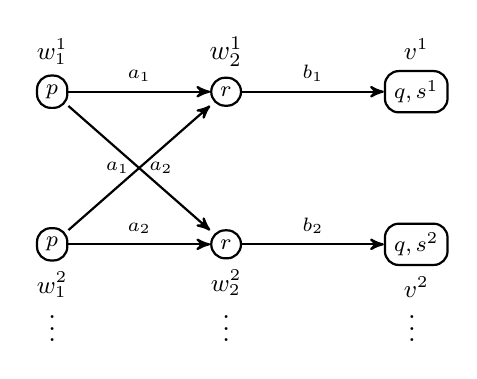
\begin{tikzpicture}[->]
\node [state, label=above:\small$w^1_1$] (w11) {$p$};
\node [state, label=above:$w^1_2$, right = 1.8cm of w11] (w12) {$r$};
\node [state, label=above:\small$v^1$, right = 1.8cm of w12] (v1) {$q,s^1$};
\node [state, label=below:\small$w^2_1$, below = 1.5cm of w11] (w21) {$p$};
\node [state, label=below:\small$w^2_2$, right = 1.8cm of w21] (w22) {$r$};
\node [state, label=below:\small$v^2$, right = 1.8cm of w22] (v2) {$q,s^2$};
\node [below = 0.35cm of w21] (w31) {$\vdots$};
\node [right = 1.85cm of w31] (w32) {$\vdots$};
\node [right = 2cm of w32] (v3) {$\vdots$};

\path (w11) edge[right] node [label-edge, above] {$a_1$} (w12);
\path (w11) edge[right] node [label-edge, right] {$a_2$} (w22);
\path (w12) edge[right] node [label-edge, above] {$b_1$} (v1);

\path (w21) edge[right] node [label-edge, above] {$a_2$} (w22);
\path (w21) edge[right] node [label-edge, left] {$a_1$} (w12);
\path (w22) edge[right] node [label-edge, above] {$b_2$} (v2);
\end{tikzpicture}
\end{center}

Let $\Sigma = \set{\kh_k(p,q),\kh_k(p,r),\neg\kh_j(p,q),\kh_j(p,r),p,q,r,\mlbox{b_1} q,s^1}$ a set of formulas closed by subformulas.
The equivalence classes for the plans in $\Unc_\AGT$ are,
\begin{inlineenum}
\item $[\plans_1]_\Sigma = [\plans_3]_\Sigma = \set{\plans_1,\plans_3}$ and
\item $[\plans_2]_\Sigma = [\set{a_1}]_\Sigma= \set{a_1}$,
\end{inlineenum}
for agent $k$, and $[\set{a_2}] = [\plans_4] = \setof{\set{a_i}}{i \in \natnum}$ for agent $j$.
Notice that $[\plans_1]_\Sigma$ encompasses the set of plans that are witnesses for $\kh_k(p,q)$, while $[\plans_2]_\Sigma$ encompasses the witneess for $\kh_k(p,r)$. For the case of $\kh_j(p,q)$ there is no witness under consideration, as the formula does not hold at $\modults$.   
And for $\kh_j(p,r)$, we have $[\set{a_2}]$.

A possible filtration would be $\modults^f = \tup{\W^f,\R^f, \set{\Unc^f(i)}_{i\in \AGT}, \V^f}$, with: 
\begin{enumerate}
\item $\W^f := \set{[w^1_1]_\Sigma,[w^1_2]_\Sigma,[v^1]_\Sigma,[v^2]_\Sigma}$, where:
    \begin{itemize}
        \item $[w^1_1]_\Sigma=\setof{w^i_1}{i \in \natnum}$,
        \item $[w^1_2]_\Sigma=\setof{w^i_2}{i \in \natnum}$, 
        \item $[v^1]_\Sigma=\set{v^1}$, 
        and 
        \item $[v^2]_\Sigma=\setof{v^i}{i \in \natnum \setminus \set{1}}$.
    \end{itemize}
\item $\V^f([w^1_1]_\Sigma) = \set{p}$, $\V([w^1_2]_\Sigma) = \set{r}$, $\V([v^1]_\Sigma) = \set{q,s^1}$ and $\V([v^2]_\Sigma) = \set{q}$.
\item
$\Unc^f(k) = \set{\set{a_{[\plans_1]_\Sigma}}, \set{a_{[\plans_2]_\Sigma}}, \set{a_\emptyset}}$,
$\Unc^f(j) = \set{\set{a_{[\plans_4]_\Sigma}}, \set{a_\emptyset}}$;
% $\Unc^f(k) = \set{\set{a_\emptyset}}$;
\item $\R^f$ is defined as follows for each $a \in \ACT^\Sigma$:
\begin{itemize}
\item $\R^f_{a_\emptyset} = \emptyset$,
\item $\R^f_{a_{[\plans_1]_\Sigma}} = \setof{([w^1_1]_\Sigma,[v^i]_\Sigma)}{i \in \natnum}$ (if $G_{[\plans_1]_\Sigma} = [\plans_1]_\Sigma$),
\item $\R^f_{a_{[\plans_2]_\Sigma}} = \set{([w^1_1]_\Sigma,[w^1_2]_\Sigma)}$ (if $G_{[\plans_2]_\Sigma} = [\plans_2]_\Sigma$),
\item $\R^f_{a_{[\plans_2]_\Sigma}} = \set{([w^1_1]_\Sigma,[w^1_2]_\Sigma)}$ (if $G_{[\plans_4]_\Sigma} = [\plans_4]_\Sigma$), and 
\item $\R^f_{b_1} = \set{([w^1_2]_\Sigma,[v^1]_\Sigma)}$. % (given $\ACT^\Sigma_\square = \set{b_1}$)
\end{itemize}
\end{enumerate}

\medskip

The filtration $\modults^f$ is depicted below:

\begin{center}
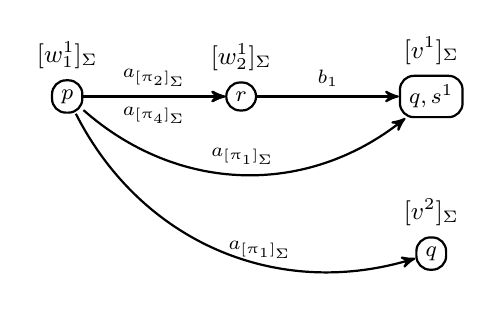
\begin{tikzpicture}[->]
\node [state, label=above:\small{$[w^1_1]_\Sigma$}] (w11) {$p$};
\node [state, label=above:\small{$[w^1_2]_\Sigma$}, right = 1.8cm of w11] (w12) {$r$};
\node [state, label=above:\small{$[v^1]_\Sigma$}, right = 1.8cm of w12] (v1) {$q,s^1$};
\node [state, label=above:\small{$[v^2]_\Sigma$}, below = 1.5cm of v1] (v2) {$q$};
% \node [below = 0.1cm of v2] (v3) {$\vdots$};
% \node [below = 1.8cm of w12] (w32) {$\vdots$};

\path (w11) edge[right] node [label-edge, above] {$a_{[\plans_2]_\Sigma}$} (w12);
\path (w11) edge[right] node [label-edge, below] {$a_{[\plans_4]_\Sigma}$} (w12);
\path (w11) edge[below, bend right=40] node [label-edge, above] {$a_{[\plans_1]_\Sigma}$} (v1);
\path (w11) edge[right, bend right=40] node [label-edge, right] {$a_{[\plans_1]_\Sigma}$} (v2);
\path (w12) edge[right] node [label-edge, above] {$b_1$} (v1);
\end{tikzpicture}
\end{center}

If, however, we consider $G_{[\plans_1]_\Sigma} = \set{\plans_1}$, then $\R^f_{a_{[\plans_1]_\Sigma}} = \set{([w^1_1]_\Sigma,[v^1]_\Sigma)}$ as $(w^1_1,v^1)$ is the only edge that holds the two conditions.
\end{example}

\medskip

We then proceed to prove that, given a model and its filtration via $\Sigma$, they both satisfy the same formulas in $\Sigma$.

\medskip

\begin{theorem}\label{th:filtration}
Let $\modults = \tup{\W,\R, \set{\Unc(i)}_{i\in \AGT}, \V}$ be an \ults and
let $\Sigma$ be a set of $\KHiMLlogic$-formulas that is closed under subformulas.
Then, for all $\psi \in \Sigma$ and $w \in \W$, 
\[
    \modults,w\models \psi \ \mbox{  iff  } \ \modults^f,[w]_\Sigma\models \psi.
\] 
Moreover, if $\Sigma$ is finite then $\modults^f$ is a finite model.
\end{theorem}

\begin{proof}
Boolean cases work as expected. We will proceed to prove the cases for the modalities $\khi$ and $\mlbox{a}$.

\begin{itemize}
\item \textbf{Case $\khi(\psi,\varphi)$}:

$(\Rightarrow)$ Suppose $\modults \models \khi(\psi,\varphi)$, and let $\plans \in \Unc(i)$ be one of its witnesses.
By~\Cref{def:filtration-actions}, $a_{[\plans]_\Sigma} \in \ACT^\Sigma_i$ and thus, $\set{a_{[\plans]_\Sigma}} \in \Unc^f(i)$. It is enough to prove that this is a witness for $ \khi(\psi,\varphi)$ in $\modults^f$. 
By \Cref{item:khiml-fil} of~\Cref{def:filtrations}, for all $\plans' \in G_{[\plans]_\Sigma}$, $\plans \planequiv_\Sigma \plans'$.
Then, for all $\plans' \in G_{[\plans]_\Sigma}$, $\truthset{\modults}{\psi} \subseteq \stexec(\plans')$ and $\R_{\plans'}(\truthset{\modults}{\psi}) \subseteq \truthset{\modults}{\varphi}$.
    \begin{enumerate}
        \item Let $[w]_\Sigma \in \truthset{\modults^f}{\psi}$. By inductive hypothesis, for all $w' \in [w]_\Sigma = [w']_\Sigma$, $w' \in \truthset{\modults}{\psi}$,  thus $[w]_\Sigma \subseteq \stexec(\plans')$, for all $\plans' \in G_{[\plans]_\Sigma}$.
        Then, $[w]_\Sigma \in \stexec(a_{[\plans]_\Sigma})$. Therefore, $\truthset{\modults^f}{\psi} \subseteq \stexec(\set{a_{[\plans]_\Sigma}})$.

        \item Let $([w]_\Sigma,[v]_\Sigma) \in \R^f_{a_{[\plans]_\Sigma}}$ be such that $[w]_\Sigma \in \truthset{\modults^f}{\psi}$.
        Then, for some $w' \in [w]_\Sigma = [w']_\Sigma$, $v' \in [v]_\Sigma = [v']_\Sigma$ and $\plans' \in G_{[\plans]_\Sigma}$ we have $(w',v') \in \R_{\plans'}$.
        By inductive hypothesis, $w' \in \truthset{\modults}{\psi}$ and thus $v' \in \truthset{\modults}{\varphi}$.
        Again, by inductive hypothesis, $[v']_\Sigma = [v]_\Sigma \in \truthset{\modults^f}{\varphi}$.
        Then, $\R^f_{\set{a_{[\plans]_\Sigma}}}(\truthset{\modults^f}{\psi}) \subseteq \truthset{\modults^f}{\varphi}$.
    \end{enumerate}

A a consequence, we get $\modults^f \models \khi(\psi,\varphi)$. \\

$(\Leftarrow)$ Suppose $\modults^f \models \khi(\psi,\varphi)$, and let $\plans \in \Unc^f(i)$ be one of its witnesses. 
If $\plans = \set{a_\emptyset}$, then $\truthset{\modults^f}{\psi} \subseteq \stexec(\set{a_\emptyset}) = \emptyset$.
By inductive hypothesis, $\truthset{\modults}{\psi} = \emptyset$ and any $\plans \in \Unc(i)$ is a witness in $\modults$ for $\khi(\psi,\varphi)$. 
If $\plans = \set{a_{[\plans']_{\Sigma}}}$, then $\truthset{\modults^f}{\psi} \subseteq \stexec(\set{a_{[\plans']_\Sigma}})$ and $\R^f_{\set{a_{[\plans']_\Sigma}}}(\truthset{\modults^f}{\psi}) \subseteq \truthset{\modults^f}{\varphi}$.
It is enough to prove that any $\plans'' \in G_{[\plans']_\Sigma}$ does the job.

    \begin{enumerate}
        \item Let $w \in \truthset{\modults}{\psi}$, by inductive hypothesis, $[w]_\Sigma \in \truthset{\modults^f}{\psi}$ and consequently $[w]_\Sigma \in \stexec(\set{a_{[\plans']_\Sigma}})$.
        By \Cref{item:khiml-fil} in~\Cref{def:filtrations}, we have that $[w]_\Sigma \subseteq \bigcap_{\plans'' \in G_{[\plans']_\Sigma}} \stexec(\plans'')$, and naturally that $w \in \bigcap_{\plans'' \in G_{[\plans']_\Sigma}} \stexec(\plans'')$.
        Thus, $\truthset{\modults}{\psi} \subseteq \stexec(\plans'')$, for all $\plans'' \in G_{[\plans']_\Sigma}$.

        \item Let $(w,v) \in \R_{\plans''}$ such that $w \in \truthset{\modults}{\psi}$.
        Since $w \in \bigcap_{\plans'' \in G_{[\plans']_\Sigma}} \stexec(\plans'')$, necessarily we have $([w]_\Sigma,[v]_\Sigma) \in \R^f_{a_{[\plans']_\Sigma}}$.
        By inductive hypothesis, $[w]_\Sigma \in \truthset{\modults^f}{\psi}$ and with this $[v]_\Sigma \in \truthset{\modults^f}{\varphi}$.
        Again, by inductive hypothesis, $v \in \truthset{\modults}{\varphi}$. Then, $\R_{\plans''}(\truthset{\modults}{\psi}) \subseteq \truthset{\modults}{\varphi}$, for any $\plans'' \in G_{[\plans']_\Sigma}$.
    \end{enumerate}

Therefore, $\modults \models \khi(\psi,\varphi)$. 

\item \textbf{Case $\mlbox{a}\varphi$}: $(\Rightarrow)$ Suppose $\modults,w \models \mlbox{a}\varphi$.
Let $([w]_\Sigma,[v]_\Sigma) \in \R^f_a$, since $\mlbox{a}\varphi \in \Sigma$, then $\modults,v \models \varphi$.
By IH, $\modults^f,[v]_\Sigma \models \varphi$.
Hence, $\modults^f,[w]_\Sigma \models \mlbox{a}\varphi$.

$(\Leftarrow)$ Suppose $\modults^f,[w]_\Sigma \models \mlbox{a}\varphi$.
Let $(w,v) \in \R_a$, then $([w]_\Sigma,[v]_\Sigma) \in \R^f_a$ and $\modults^f,[v]_\Sigma \models \varphi$.
By IH, $\modults,v \models \varphi$.
Hence, $\modults,w \models \mlbox{a}\varphi$.
\end{itemize}

It remains to show that if $\Sigma$ is finite, then $\modults^f$ is finite.
First, note that the number of elements in $\W^f$ is at most exponential in the size in the number of formulas in $\Sigma$.
Thus, $\W^f$ and $\V^f$ are finite. Similarly, as the number of $\khi(\psi,\varphi)$ and $\mlbox{a} \varphi$ in $\Sigma$ are finite, $\ACT^{\Sigma}$ is also finite.
Thus, $\R^f$ and $\Unc^f$ are both finite, and therefore $\modults^f$ is a finite model.
\end{proof}

\medskip 

\begin{example}\label{ex:filtration-preserves}
 Consider again~\Cref{ex:afiltration}. Notice that the filtration preserves the satisfiability of formulas in $\Sigma$. For instance, $\modults\models\kh_k(p,q)$ with $\plans_1$ as witness, while $\modults^f\models\kh_k(p,q)$ with $[\plans_1]_\Sigma$ as witness. Also, it is clear that both $\modults\not\models\kh_j(p,q)$ and $\modults^f\not\models\kh_j(p,q)$, and that $\modults,w^1_2\models[b_1]q$ and $\modults^f,[w^1_2]_\Sigma\models[b_1]q$.
\end{example}

\medskip

Considering~\Cref{th:filtration}, it remains to prove that, given a model $\modults$ and a set of formulas $\Sigma$ closed under subformulas, the set of filtrations of $\modults$ via $\Sigma$ is non empty.
This can be achieved by defining $G_{[\plans]_\Sigma} = [\plans]_\Sigma \neq \emptyset$ for each $a_{[\plans]_\Sigma} \in \ACT^\Sigma_i$, and considering at least one of the two alternatives to define $\R_a$ for each $a \in \ACT^\Sigma_\square$ given in \cite{HML,mlbook}:

\begin{itemize}
\item $([w]_\Sigma,[v]_\Sigma) \in \R^f_a$ iff there exists $w' \in [w]_\Sigma$, $v' \in [v]_\Sigma$ such that $(w',v') \in \R_a$; or
\item $([w]_\Sigma,[v]_\Sigma) \in \R^f_a$ iff for all $\mlbox{a}\varphi \in \Sigma$, $\modults,w \models \mlbox{a}\varphi$ then $\modults,v \models \varphi$.
\end{itemize}
 
\medskip

The last theorem states that every satisfiable formula of $\KHiMLlogic$, is satisfiable in a finite model.
As a consequence, the satisfiability problem for $\KHiMLlogic$ is decidable.

\medskip

\begin{corollary}\label{cor:extended-decidable}
The satisfiability problem for $\KHiMLlogic$ is decidable.
\end{corollary}

\begin{proof}
Suppose $\varphi$ is satisfiable, then there exists a model $\modults$ and a state $w$ such that $\modults,w\models\varphi$. Let $\Sigma$ be the set of subformulas of $\varphi$ (including $\varphi$). Then, by~\Cref{th:filtration}, $\modults^\Sigma,[w]_\Sigma\models\varphi$. Since $\Sigma$ is finite, $\modults^\Sigma$ is finite, and of size at most exponential. Consequently, we know there exists a finite model of $\varphi$. Thus, we can list all the models and try one by one, whether they satisfy $\varphi$ or not, by calling a model-checking algorithm. Since model-checking is decidable (by simply combining the algorithm for basic modal logic~\cite{mlbook}, and the one for $\KHilogic$~\cite{AFSVQ21,AFSVQ23report}), the corollary follows. \raul{No tenemos demo especifica de que model-checking es decidible, dejamos asi como esta?}
\end{proof}

\medskip

It is worth noticing that the conditions regarding the treatment of $\Unc^f(i)$ in~\Cref{def:filtrations} are slightly different from the conditions introduced in~\cite{AFSVQ23report} for the basic logic $\KHilogic$. Therein, the existence of a filtration is not established. Thus, in this work we update the definition of filtrations, making easier to guarantee that always we can obtain a finite model from any set of finite formulas, and consequently~\Cref{cor:extended-decidable}.

% The rest of the section will be devoted to introduce a new family of dynamic epistemic logics extending $\KHiMLlogic$.


% \subsection{Atomic action refinement}
\label{subsec:atom-ref}

The main goal of defining the extended logic $\KHiMLlogic$ is to obtain enough expressivity to axiomatize some dynamic modalities. Here, we define the modality $\srefbox{a}$, inspired by the refinement modality from~\Cref{sec:ref}. A formula $\srefbox{a}\varphi$ publicly establishes that action $a$ must be distinguished from any other, and in such a context $\varphi$ holds. Unlike the modality $\refbox{\plan_1}{\plan_2}$, this modality takes atomic actions but we will generalize it later to arbitrary plans. 
%The operator models the case This is useful as for instance, an uninformed agent may receive a concrete information about the actual effect of a particular action, thus this action becomes distinguishable from any other. Moreover, in case the agent is oblivious about the existence of an action, she becomes aware of it as a result of the announcement. We formalize these ideas below.

\medskip

\begin{definition}\label{def:ssrefsyntax}
Formulas of the language $\AtomReflogic$ are defined by the following grammar:
\[
\varphi ::= p \mid \neg\varphi \mid \varphi\vee\varphi \mid \khi(\varphi,\varphi) \mid \mlbox{a}\varphi \mid \srefbox{a}\varphi,
\]
with $p \in \PROP$, $i\in\AGT$ and $a \in \ACT$. Formulas of the form $\srefbox{a}\varphi$ are read as: \emph{``after announcing that $a$ is distinguishable from any other plan, $\varphi$ holds''.} 
\end{definition}

\medskip

\begin{definition}\label{def:ssrefsemantics}
Let $\modults = \tup{\W, \R, \Unc, \V}$ be an \ults, $a \in \ACT$ and let $\varphi$ be an  $\PlanReflogic$-formula,
\[
\modults,w \models \srefbox{a}\varphi \ \ \iff \ \ \modults^a,w \models \varphi,
\] 
where $\modults^a = \tup{\W,\R,\Unc',\V}$, with:
\begin{itemize}
\item $\Unc'(i) = (\Unc(i) \setminus \set{\plans}) \cup \set{\set{a}}$, if there is $\plans \in \Unc(i)$ such that $a \in \plans$,
\item $\Unc'(i) = \Unc(i) \cup \set{\set{a}}$ otherwise.
\end{itemize}
\end{definition}

\medskip

Intuitively, the new dynamic modality is an announcement of the fact that a given action has a behavior that can be uniquely determined. In case the action is not a part of the actions that are under the consideration of a certain agent, it is added to it, making the agent aware of its existence. 
The following proposition states that the new modality is self-dual and normal.

\medskip

\begin{proposition} The following propositions hold:
\begin{enumerate}
\item $\models \srefbox{a}\varphi \lra \neg\srefbox{a}\neg\varphi$. 
\item $\models \srefbox{a}(\varphi_1 \ra \varphi_2) \ra (\srefbox{a}\varphi_1 \ra \srefbox{a}\varphi_2)$.
\item If $\models \varphi$, then $\models \srefbox{a}\varphi$.
\end{enumerate}
\end{proposition}

\medskip

Let us introduce now an example of use of the new modality.

\medskip

\begin{example}
Let $\modults$ be the single agent model depicted below, with $\Unc(i):=\set{\set{a}}$. It is clear that $\modults,w\not\models\khi(p,q)$. But we have that $\modults,w\models[!b]\khi(p,q)$, as after announcing $b$, the agent becomes aware of the existence of that plan, and she can use it to guarantee $q$ given~$p$. 
\begin{center}
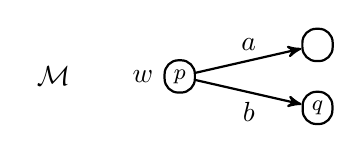
\begin{tikzpicture}[->, grow' = right, level/.style={sibling distance = 2em/#1}, level distance = 1.5em]
\node[state] at (0,1) (p) [label=left:$w$]{$p$};
\node[left = of p] (m) {$\modults$};
\node[state] at (1.75,0.6) (nq) {{$q$}};
\node[state] at (1.75,1.4) (q) {\phantom{$p$}};
\path (p) edge [above] node {$a$} (q);
\path (p) edge [below] node {$b$} (nq);
\end{tikzpicture} 
\end{center} 
\end{example}

We proceed now to introduce a complete axiom system for $\AtomReflogic$. In this case, the expressive power of the underlying static logic is sufficient to capture the behavior of $\srefbox{a}$, and we can obtain an axiomatization via reduction axioms.

Reduction axioms can be used to translate every formula of $\AtomReflogic$ into an equivalent formula of $\KHiMLlogic$. The challenging case is, as usual, to eliminate the occurence of a $\srefbox{a}$ modality in presence of $\khi$. Consider a formula $\srefbox{a}\khi(\psi,\varphi)$. After the ``announcement'' of action $a$ being different to any other plan, there are two possible reasons of why $\khi(\psi,\varphi)$ holds. The first possibility, is that action $a$ plays no role in the truth of $\khi(\psi,\varphi)$. In this case, we can push the dynamic modality into the front of the pre and post-conditions of the $\khi$ modality, i.e., we obtain $\khi(\srefbox{a}\psi,\srefbox{a}\varphi)$. The second possibility is that $a$ is crucial in order to raise new knowledge for the agent. If the singleton $\set{a}$ is the witness for $\khi(\psi,\varphi)$ it is because: 1) $a$ is SE at every state satisfying $\psi$ after the annoucement of $a$ (notice that as $a$ is a single action, SE is equivalent to executability); and 2) from every $\psi$-state, after every execution of $a$ we always get that $\varphi$ holds (in the model updated by $\srefbox{a}$). The former is captured in formula by $\srefbox{a}\psi\ra\mldiam{a}\top$ holding everywhere, while the latter is captured by $\mlbox{a}\srefbox{a}\varphi$. Putting all together, this case is reflected by $\A(\srefbox{a}\psi\ra(\mldiam{a}\top\wedge\mlbox{a}\srefbox{a}\varphi))$. 

%The other cases are standard reductions, so we obtain the axioms shown in~\Cref{tab:ssrefaxiom}.

\begin{table}[t]
\begin{tabular}{l@{\quad}l}
\toprule
\axm{RAtom} & $\vdash \srefbox{a}p \lra p$ \\
\axm{R$\neg$} & $\vdash \srefbox{a} \neg \varphi_1 \lra \neg \srefbox{a} \varphi_1$ \\
\axm{R$\vee$} & $\vdash \srefbox{a} (\varphi_1 \vee \varphi_2) \lra (\srefbox{a} \varphi_1 \vee \srefbox{a} \varphi_2)$ \\
\axm{R$\square$} & $\vdash \srefbox{a}\mlbox{a}\varphi_1 \lra \mlbox{a}\srefbox{a}\varphi_1$ \\
\axm{RKh} & $\vdash \srefbox{a} \khi(\varphi_1,\varphi_2) \lra (\khi(\srefbox{a} \varphi_1,\srefbox{a} \varphi_2) \vee \A(\srefbox{a} \varphi_1 \ra (\mldiam{a}\top \wedge \mlbox{a} \srefbox{a}\varphi_2)))$ \\
\axm{RE$_{\srefbox{}}$} & $\text{From } \vdash \varphi \leftrightarrow \psi \text{ derive } \vdash \srefbox{a}\varphi \leftrightarrow \srefbox{a}\psi$ \\
\bottomrule
\end{tabular}
\caption{Reduction axioms $\axset_{\AtomReflogic}$.}\label{tab:ssrefaxiom}
\end{table}

\medskip 

\begin{proposition}\label{pro:ssrefaxioms} The reduction axioms from~\Cref{tab:ssrefaxiom} are valid.
% \begin{enumerate}
% \item $\models \srefbox{a}p \lra p$
% \item $\models \srefbox{a} \neg \varphi_1 \lra \neg \srefbox{a} \varphi_1$
% \item $\models \srefbox{a} (\varphi_1 \vee \varphi_2) \lra (\srefbox{a} \varphi_1 \vee \srefbox{a} \varphi_2)$
% \item $\models \srefbox{a}\mlbox{a}\varphi_1 \lra \mlbox{a}\srefbox{a}\varphi_1$
% \item $\models \srefbox{a} \khi(\varphi_1,\varphi_2) \lra (\khi(\srefbox{a} \varphi_1,\srefbox{a} \varphi_2) \vee \A(\srefbox{a} \varphi_1 \ra (\mldiam{a}\top \wedge \mlbox{a} \srefbox{a}\varphi_2)))$
% \end{enumerate}
\end{proposition}
\begin{proof}
We only discuss validity of the axiom $\axm{RKh}$. 
Let $\modults = \tup{\W, \R, \Unc, \V}$ be an \ults.

$\Rightarrow)$ $\modults \models \srefbox{a} \khi(\varphi_1,\varphi_2)$ iff $\modults^a \models \khi(\varphi_1,\varphi_2)$ iff there is $\plans' \in \Unc'(i)$ s.t. $\truthset{\modults^a}{\varphi_1} \subseteq \stexec^{\modults^a}(\plans')$ and $\R_{\plans'}(\truthset{\modults^a}{\varphi_1}) \subseteq \truthset{\modults^a}{\varphi_2}$.
Using $\truthset{\modults^a}{\psi} = \truthset{\modults}{\srefbox{a} \psi}$ and $\stexec^{\modults^a}(\plans') = \stexec^\modults(\plans')$ (since relations remain unchanged), this is equivalent to the existence of $\plans' \in \Unc'(i)$ s.t. $\truthset{\modults}{\srefbox{a} \varphi_1} \subseteq \stexec^\modults(\plans')$ and $\R_{\plans'}(\truthset{\modults}{\srefbox{a} \varphi_1}) \subseteq \truthset{\modults}{\srefbox{a} \varphi_2}$. We need to consider two cases:
\begin{itemize}
\item If $\plans' \neq \set{a}$, then $\plans' \in \Unc(i)$ and we get $\modults \models \khi(\srefbox{a}\varphi_1,\srefbox{a}\varphi_2)$.
\item If $\plans' = \set{a}$, then $\truthset{\modults}{\srefbox{a}\varphi_1} \subseteq \stexec^\modults(a)$ and $\R_a(\truthset{\modults}{\srefbox{a}\varphi_1}) \subseteq \truthset{\modults}{\srefbox{a}\varphi_2}$.
From the first part, using the definition of SE, we can derive that for all $w \in \truthset{\modults}{\srefbox{a}\varphi_1}$, we have $\modults,w \models \mldiam{a}\top$.
From the second one, we can reach that for all $w \in \truthset{\modults}{\srefbox{a}\varphi_1}$, $\modults,w \models \mlbox{a} \srefbox{a}\varphi_2$.
Thus, for all $w \in \W$, $\modults,w \models \srefbox{a} \varphi_1 \ra (\mldiam{a}\top \wedge \mlbox{a} \srefbox{a}\varphi_2)$.
\end{itemize}

$\Leftarrow)$ Suppose $\modults \models \khi(\srefbox{a} \varphi_1,\srefbox{a} \varphi_2) \vee \A(\srefbox{a} \varphi_1 \ra (\mldiam{a}\top \wedge \mlbox{a} \srefbox{a}\varphi_2))$. We consider two cases:
\begin{itemize}
    \item $\modults \models \khi(\srefbox{a} \varphi_1,\srefbox{a} \varphi_2)$: Let $\plans \in \Unc(i)$ be s.t. $\truthset{\modults}{\srefbox{a}\varphi_1} \subseteq \stexec^\modults(\plans)$ and $\R_\plans(\truthset{\modults}{\srefbox{a}\varphi_1}) \subseteq \truthset{\modults}{\srefbox{a}\varphi_2}$.
    As stated before, this is equivalent to $\truthset{\modults^a}{\varphi_1} \subseteq \stexec^{\modults^a}(\plans)$ and $\R_\plans(\truthset{\modults^a}{\varphi_1}) \subseteq \truthset{\modults^a}{\varphi_2}$.
    If $a \notin \plans$, then $\plans \in \Unc'(i)$.
    If $a \in \plans$, then $\set{a} \in \Unc'(i)$, $\stexec^{\modults^a}(\plans) \subseteq \stexec^{\modults^a}(\set{a})$ and $\R_{\set{a}}(\truthset{\modults^a}{\varphi_1}) \subseteq \R_\plans(\truthset{\modults^a}{\varphi_1})$. In any case, we get $\modults \models \srefbox{a}\khi(\varphi_1,\varphi_2)$.

    \item $\modults \models \A(\srefbox{a} \varphi_1 \ra (\mldiam{a}\top \wedge \mlbox{a} \srefbox{a}\varphi_2))$: Notice that $a$ meets the strong executability and reachability conditions.
    We only need to prove that $\set{a} \in \Unc'(i)$. But this is always the case. Hence,  $\modults \models \srefbox{a}\khi(\varphi_1,\varphi_2)$.
\end{itemize}
\end{proof}

Now, using~\Cref{th:cm-ults-khikt-completeness}, the following result easily follows.

\medskip 

\begin{theorem}\label{th:sscomplete}
The axiom system $\axset_{\AtomReflogic}+\axset_{\khi,\square}$ for $\AtomReflogic$ is sound and strongly complete w.r.t. the class of all models.
\end{theorem}

\medskip 

Finally, as the elimination of the dynamic modality takes a finite number of steps, using~\Cref{cor:extended-decidable} we can conclude:

\medskip 

\begin{corollary}
The satisfiability problem for $\AtomReflogic$ is decidable.
\end{corollary} 


\subsection{Plan refinement}
\label{sec:planref}

The idea introduced in the previous section has the novelty of admitting a sound and complete axiom system, a property that was missing in other approaches. However, one can argue that allowing action refinement only, is a bit limited. But, is this a real limitation of the framework? Or these ideas can actually be generalized to arbitrary plans? In this section we show that the latter is the case. Moreover, we show that all the results presented for $\AtomReflogic$ naturally extend to this case.
We start by presenting the syntax and semantics of the new logic. 

\begin{definition}\label{def:srefsyntax}
Formulas of the language $\PlanReflogic$ are given by
\[
\varphi ::= p \mid \neg\varphi \mid \varphi\vee\varphi \mid \khi(\varphi,\varphi) \mid \mlbox{a}\varphi \mid \srefbox{\plan}\varphi,
\]
with $p \in \PROP$, $i\in\AGT$, $a \in \ACT$ and $\plan \in \ACT^*$.  Formulas of the form $\srefbox{\plan}\varphi$ are read as: \emph{``after announcing that $\plan$ is distinguishable from any other plan, $\varphi$ holds''.} 
\end{definition}

\begin{definition}\label{def:srefsemantics}
Let $\modults = \tup{\W, \R, \Unc, \V}$ be an \ults, $\plan \in \ACT^*$ and  be a $\PlanReflogic$-formula,
\[
\modults,w \models \srefbox{\plan}\varphi \ \ \iff \ \ \modults^\plan,w \models \varphi,
\]
where $\modults^\plan = \tup{\W,\R,\Unc',\V}$, with:
\begin{itemize}
\item $\Unc'(i) = (\Unc(i) \setminus \set{\plans}) \cup \set{\set{\plan}}$ if there is $\plans \in \Unc(i)$ such that $\plan \in \plans$,
\item $\Unc'(i) = \Unc(i) \cup \set{\set{\plan}}$ otherwise.
\end{itemize}
\end{definition}

The refinement in $\modults^\plan$ is essentially as in~\Cref{def:ssrefsemantics} except that now we allow arbitrary plans. This generalization enables us e.g. to handle the example we have been using along the paper.

\begin{example}\label{ex:sref}
Recall the model $\modults$ from \Cref{ex:cook}.
Now, suppose that a cooking professor teaches (announces) to both agents about the plan $\mathit{ebmfsp}$.
Now every agent is able to distinguish the plan $\mathit{ebmfsp}$ from all others.
Moreover, after the announcement, agent $j$ knows how to make a good cake.
Thus, $\modults \models \srefbox{\mathit{ebmfsp}} \kh_j(h,g)$.
\end{example}

Again, we can state the following properties:
\begin{proposition}
The following hold:
\begin{enumerate}
\item $\models \srefbox{\plan}\varphi \lra \neg\srefbox{\plan}\neg\varphi$. 
\item $\models \srefbox{\plan}(\varphi_1 \ra \varphi_2) \ra (\srefbox{\plan}\varphi_1 \ra \srefbox{\plan}\varphi_2)$
\item If $\models \varphi$, then $\models \srefbox{\plan}\varphi$
\end{enumerate}
\end{proposition}
% \begin{proof}
% Let $\modults = \tup{\W, \R, \Unc, \V}$ be an \ults.
% \begin{enumerate}
% \item Suppose $\modults,w \models \srefbox{\plan}(\varphi_1 \ra \varphi_2) \wedge \srefbox{\plan}\varphi_1$
% \end{enumerate}
% \end{proof}

\subsubsection{Axiom System}

Now it is time to investigate a complete axiomatization for $\PlanReflogic$, one of the main goals of introducing this framework over an extended basic language. As shown in what follows, the elimination of the dynamic modality $\srefbox{\plan}$ in presence of the modality $\khi$ requires a little bit more of work than the single action case we presented already.  The case in which the announcement does not affect the knowledge, is straightforward. For the other case, we need to make sure than for every state in which after the announcement of $\plan$ guarantees that if the precondition holds ($\srefbox{\plan}\varphi_1$), then $\plan$ is SE and after its execution, the postcondition holds ($\srefbox{\plan}\varphi_2$). The latter, is expressed by the predicate $P(\plan,\srefbox{\plan}\varphi_2)$, described below. Notice that $P$ can be defined as we extended the expressivity of the underlying language, by allowing basic action modalities.
\begin{table}[t]
\begin{tabular}{l@{\quad}l}
\toprule
\axm{RAtom} & $\vdash \srefbox{\plan}p \lra p$ \\
\axm{R$\neg$} & $\vdash \srefbox{\plan} \neg \varphi_1 \lra \neg \srefbox{\plan} \varphi_1$ \\
\axm{R$\vee$} & $\vdash \srefbox{\plan} (\varphi_1 \vee \varphi_2) \lra (\srefbox{\plan} \varphi_1 \vee \srefbox{\plan} \varphi_2)$ \\
\axm{R$\square$} & $\vdash \srefbox{\plan}\mlbox{a}\varphi_1 \lra \mlbox{a}\srefbox{\plan}\varphi_1$ \\
\axm{RKh} & $\vdash \srefbox{\plan} \khi(\varphi_1,\varphi_2) \lra (\khi(\srefbox{\plan} \varphi_1,\srefbox{\plan} \varphi_2) \vee \A(\srefbox{\plan} \varphi_1 \ra P(\plan,\srefbox{\plan}\varphi_2)))$ \\
\axm{RE$_{\srefbox{}}$} & $\text{From } \vdash \varphi \leftrightarrow \psi \text{ derive } \vdash \srefbox{\plan}\varphi \leftrightarrow \srefbox{\plan}\psi$ \\
\bottomrule
\end{tabular}
\caption{Reduction axioms $\axset_{\PlanReflogic}$.}\label{tab:srefaxiom}
\end{table}

\begin{proposition}\label{pro:srefaxioms}
Let $\beta \in \ACT^*$, we define the extension of $\mlbox{a}$ for plan, $\mlbox{\beta}$ as
\[
\mlbox{\beta} \psi = 
\begin{cases}
\psi &\quad \beta = \epsilon\\
\mlbox{\beta[1]} \dots \mlbox{\beta[\card{\beta}]} \psi &\quad \beta \neq \epsilon \\
\end{cases}
\]
With this, let $P$ be defined inductively as: 
\[
    \begin{array}{lcl}
        P(\epsilon,\psi) & = & \psi \\
        P(\alpha,\psi)  &= &(\bigwedge_{k=0}^{\card{\alpha}-1}(\mlbox{\alpha_k}\mldiam{\alpha[k+1]}\top) \wedge \mlbox{\alpha} \psi), \mbox{ with } \mlbox{\beta} = \mlbox{\beta[1]} \dots \mlbox{\beta[\card{\beta}]}. 
    \end{array}
\]
Then, the reduction axioms from~\Cref{tab:srefaxiom} are valid.
% \begin{enumerate}
% \item $\models \srefbox{\plan}p \lra p$
% \item $\models \srefbox{\plan} \neg \varphi_1 \lra \neg \srefbox{\plan} \varphi_1$
% \item $\models \srefbox{\plan} (\varphi_1 \vee \varphi_2) \lra (\srefbox{\plan} \varphi_1 \vee \srefbox{\plan} \varphi_2)$
% \item $\models \srefbox{\plan}\mlbox{a}\varphi_1 \lra \mlbox{a}\srefbox{\plan}\varphi_1$
% \item $\models \srefbox{\plan} \khi(\varphi_1,\varphi_2) \lra (\khi(\srefbox{\plan} \varphi_1,\srefbox{\plan} \varphi_2) \vee \A(\srefbox{\plan} \varphi_1 \ra P(\plan,\srefbox{\plan}\varphi_2)))$
% \end{enumerate}
% with $P(\alpha,\psi) = (\bigwedge_{k=0}^{\card{\alpha}-1}(\mlbox{\alpha_k}\mldiam{\alpha[k+1]}\top) \wedge \mlbox{\alpha} \psi)$, $\mlbox{\beta} = \mlbox{\beta[1]}...\mlbox{\beta[\card{\beta}]}$ and $P(\epsilon,\psi) = \psi$.
\end{proposition}
\begin{proof}
The proofs ideas for the first four items are similar to the ones in \Cref{pro:ssrefaxioms}. Let us focus again in the case of $\axm{RKh}$.  
Let $\modults = \tup{\W, \R, \Unc, \V}$ be an \ults, then we prove below the two directions of the double implication.

$\Rightarrow):$ Assume $\modults \models \srefbox{\plan} \khi(\varphi_1,\varphi_2)$, i.e.,  $\modults^\plan \models \khi(\varphi_1,\varphi_2)$ iff there is $\plans' \in \Unc'(i)$ s.t. $\truthset{\modults^\plan}{\varphi_1} \subseteq \stexec^{\modults^\plan}(\plans')$ and $\R_{\plans'}(\truthset{\modults^\plan}{\varphi_1}) \subseteq \truthset{\modults^\plan}{\varphi_2}$.
Using $\truthset{\modults^\plan}{\psi} = \truthset{\modults}{\srefbox{\plan} \psi}$ and $\stexec^{\modults^\plan}(\plans') = \stexec^\modults(\plans')$ (since the relations remain unchanged), this is equivalent to say that there is $\plans' \in \Unc'(i)$ s.t. $\truthset{\modults}{\srefbox{\plan} \varphi_1} \subseteq \stexec^\modults(\plans')$ and $\R_{\plans'}(\truthset{\modults}{\srefbox{\plan} \varphi_1}) \subseteq \truthset{\modults}{\srefbox{\plan} \varphi_2}$. We need to consider two cases:
\begin{itemize}
\item If $\plans' \neq \set{\plan}$, then $\plans \in \Unc(i)$ and we get $\modults \models \khi(\srefbox{\plan}\varphi_1,\srefbox{\plan}\varphi_2)$.
\item If $\plans' = \set{\plan}$, then $\truthset{\modults}{\srefbox{\plan}\varphi_1} \subseteq \stexec^\modults(\plan)$ and $\R_\plan(\truthset{\modults}{\srefbox{\plan}\varphi_1}) \subseteq \truthset{\modults}{\srefbox{\plan}\varphi_2}$.
From the first part, using the definition of SE, we can derive that for all $w \in \truthset{\modults}{\srefbox{\plan}\varphi_1}$, $k \in \intint{0}{\card{\plan}-1}$ we have $\modults,w \models \mlbox{\plan_l}\mldiam{\plan[l+1]}\top$.
From the second one, we can reach that for all $w \in \truthset{\modults}{\srefbox{\plan}\varphi_1}$, $\modults,w \models \mlbox{\plan} \srefbox{\plan}\varphi_2$.
Thus, for all $w \in \W$, $\modults,w \models \srefbox{\plan} \varphi_1 \ra P(\plan,\srefbox{\plan}\varphi_2)$.
\end{itemize}

$\Leftarrow):$ Conversely, suppose $\modults \models \khi(\srefbox{\plan} \varphi_1,\srefbox{\plan} \varphi_2) \vee \A(\srefbox{\plan} \varphi_1 \ra P(\plan,\srefbox{\plan}\varphi_2))$, then the disjunction is satified by either one of the following situations:
\begin{itemize}
\item  $\modults \models \khi(\srefbox{\plan} \varphi_1,\srefbox{\plan} \varphi_2)$: Let $\plans \in \Unc(i)$ be s.t. $\truthset{\modults}{\srefbox{\plan}\varphi_1} \subseteq \stexec^\modults(\plans)$ and $\R_\plans(\truthset{\modults}{\srefbox{\plan}\varphi_1}) \subseteq \truthset{\modults}{\srefbox{\plan}\varphi_2}$.
As we already stated, this is equivalent to say that $\truthset{\modults^\plan}{\varphi_1} \subseteq \stexec^{\modults^\plan}(\plans)$ and $\R_\plans(\truthset{\modults^\plan}{\varphi_1}) \subseteq \truthset{\modults^\plan}{\varphi_2}$.
If $\plan \notin \plans$, then $\plans \in \Unc'(i)$.
If $\plan \in \plans$, then $\set{\plan} \in \Unc'(i)$, $\stexec^{\modults^\plan}(\plans) \subseteq \stexec^{\modults^\plan}(\set{\plan})$ and $\R_{\set{\plan}}(\truthset{\modults^\plan}{\varphi_1}) \subseteq \R_\plans(\truthset{\modults^\plan}{\varphi_1})$. In any case, we get $\modults \models \srefbox{\plan}\khi(\varphi_1,\varphi_2)$.

\item $\modults \models \A(\srefbox{\plan} \varphi_1 \ra P(\plan,\srefbox{\plan}\varphi_2))$: Notice that $\plan$ meets the strong executability and reachability conditions.
The only thing left to prove is that $\set{\plan} \in \Unc'(i)$. But that is direct since wheter $\plan \in \plans$ for some $\plans \in \Unc(i)$ or not, in the end $\set{\plan} \in \Unc'(i)$. Hence $\modults \models \srefbox{\plan}\khi(\varphi_1,\varphi_2)$.
\end{itemize}
\end{proof}

Thus, by again putting all the pieces together (\Cref{pro:srefaxioms,th:cm-ults-khikt-completeness}), we get:

\begin{theorem}
The axiom system $\axset_{\PlanReflogic}+\axset_{\khi,\square}$ for $\PlanReflogic$ is sound and strongly complete w.r.t. the class of all models.
\end{theorem}

By using~\Cref{,cor:extended-decidable}, we can conclude:

\begin{corollary}
$\PlanReflogic$ is decidable.
\end{corollary} \raul{revisar}



% \subsection{Semi-private plan refinement}
\label{sec:sempriv-planref}

Finally, we can consider a last type of plan refinement. Notice that, so far, the dynamic modalities we introduced produce (according to the dynamic epistemic logic terminology) ``public'' updates. This means, that the information which is revealed is accessible to all the agents, similar to what is done in public annoucements (\cite{Plaza89:lopc}). However, other kinds of communication are possible, as the so-called semi-private and private communications, achieved via e.g. action models (see e.g.~\cite{BR16}). The flexibility of our framework enables us to also doing so. In this section, we will adapt the plan refinement modality from~\Cref{def:ssrefsyntax} in order to produce a semi-private update.

\medskip 

\begin{definition}\label{def:srefgsyntax}
Formulas of the language $\AgentReflogic$ are given by
\[
\varphi ::= p \mid \neg\varphi \mid \varphi\vee\varphi \mid \khi(\varphi,\varphi) \mid \mlbox{a}\varphi \mid \srefbox{\plan,i}\varphi,
\]
with $p \in \PROP$, $i\in\AGT$, $a \in \ACT$ and $\plan \in \ACT^*$. The modality $\srefbox{\plan,i}\varphi$ is read as \emph{``after it is announced to agent $i$ that the plan $\plan$ is distinguishable from any other plan, $\varphi$ holds''.}
\end{definition}

\medskip 

\begin{definition}\label{def:srefgsemantics}
Let $\modults = \tup{\W, \R, \Unc, \V}$ be an \ults, $\plan \in \ACT^*$ and  be a $\AgentReflogic$-formula, 
\[
\modults,w \models \srefbox{\plan,i}\varphi \ \ \iff \ \ \modults^\plan_i,w \models \varphi,
\]
where $\modults^\plan_i = \tup{\W,\R,\Unc',\V}$, with:
\begin{itemize}
\item $\Unc'(j) = \Unc(j)$ if $j \neq i$,
\item $\Unc'(i) = (\Unc(i) \setminus \set{\plans}) \cup \set{\set{\plan}}$, if there is $\plans \in \Unc(i)$ such that $\plan \in \plans$,
\item $\Unc'(i) = \Unc(i) \cup \set{\set{\plan}}$ otherwise.
\end{itemize}
\end{definition}

\medskip 

\begin{example}
Suppose as in~\Cref{ex:cook}, we have an expert chef $i$, but we have two inexpert chefs $j$ and $k$, with $\Unc(j)=\Unc(k)=\set{\set{\mathit{ebfmsp},\mathit{ebmfsp}}}$. Suppose now, that agent $j$ subscribed for a course taught by agent $i$, while agent $k$ does not. Then, the information of that \textit{ebfmsp} is the correct course of action is only revealed to $j$, obtaining that $\srefbox{ebfmsp,j}\kh_j(h,g)$ while $\srefbox{ebfmsp,j}\neg\kh_k(h,g)$.
\end{example}

Again, this modality is self-dual and normal.

\medskip 

\begin{proposition} The following propositions hold:
\begin{enumerate}
\item $\models \srefbox{\plan,i}\varphi \lra \neg\srefbox{\plan,i}\neg\varphi$. 
\item $\models \srefbox{\plan,i}(\varphi_1 \ra \varphi_2) \ra (\srefbox{\plan,i}\varphi_1 \ra \srefbox{\plan,i}\varphi_2)$
\item If $\models \varphi$, then $\models \srefbox{\plan,i}\varphi$
\end{enumerate}
\end{proposition}

\medskip 

Below we state the correcteness of the reduction axioms of~\Cref{tab:srefgaxiom}, that is similar to the ``public'' cases. 

\medskip 

\begin{proposition}\label{pro:srefgaxioms}
Let $P$ be defined as in~\Cref{pro:srefaxioms}. Then, the reduction axioms from~\Cref{tab:srefgaxiom} are valid.
\end{proposition}
% \begin{enumerate}
% \item $\models \srefbox{\plan,i}p \lra p$
% \item $\models \srefbox{\plan,i} \neg \varphi_1 \lra \neg \srefbox{\plan,i} \varphi_1$
% \item $\models \srefbox{\plan,i} (\varphi_1 \vee \varphi_2) \lra (\srefbox{\plan,i} \varphi_1 \vee \srefbox{\plan,i} \varphi_2)$
% \item $\models \srefbox{\plan,i}\mlbox{a}\varphi_1 \lra \mlbox{a}\srefbox{\plan,i}\varphi_1$
% \item $\models \srefbox{\plan,i} \khi(\varphi_1,\varphi_2) \lra (\khi(\srefbox{\plan,i} \varphi_1,\srefbox{\plan,i} \varphi_2) \vee \A(\srefbox{\plan,i} \varphi_1 \ra P(\plan,\srefbox{\plan,i}\varphi_2)))$
% \item $\models \srefbox{\plan,i} \kh_j(\varphi_1,\varphi_2) \lra \kh_j(\srefbox{\plan,i} \varphi_1,\srefbox{\plan,i} \varphi_2)$
% \end{enumerate}
% with $P(\alpha,\psi) = (\bigwedge_{k=0}^{\card{\alpha}-1}(\mlbox{\alpha_k}\mldiam{\alpha[k+1]}\top) \wedge \mlbox{\alpha} \psi)$, $\mlbox{\beta} = \mlbox{\beta[1]}...\mlbox{\beta[\card{\beta}]}$ and $P(\epsilon,\psi) = \psi$.
% \end{proposition}
% \begin{proof}
% The proofs ideas for the first five items are similar to the ones in \Cref{pro:ssrefaxioms} and \Cref{pro:srefaxioms}.
% Let $\modults = \tup{\W, \R, \Unc, \V}$ be an \ults.
% \begin{enumerate}
% \item[6.] $\modults \models \srefbox{\plan,i} \kh_j(\varphi_1,\varphi_2)$ iff $\modults^\plan_i \models \kh_j(\varphi_1,\varphi_2)$ iff there is $\plans \in \Unc'(j)$ s.t. $\truthset{\modults^\plan_i}{\varphi_1} \subseteq \stexec^{\modults^\plan_i}(\plans)$ and $\R_\plans(\truthset{\modults^\plan_i}{\varphi_1}) \subseteq \truthset{\modults^\plan_i}{\varphi_2}$.
% Using $\Unc'(j) = \Unc(j)$, $\truthset{\modults^\plan_i}{\psi} = \truthset{\modults}{\srefbox{\plan,i} \psi}$ and $\stexec^{\modults^\plan_i}(\plans) = \stexec^\modults(\plans)$ (since the relations remain unchanged), this is equivalent to that there is $\plans \in \Unc(j)$ s.t. $\truthset{\modults}{\srefbox{\plan,i} \varphi_1} \subseteq \stexec^\modults(\plans)$ and $\R_\plans(\truthset{\modults}{\srefbox{\plan,i} \varphi_1}) \subseteq \truthset{\modults}{\srefbox{\plan,i} \varphi_2}$.
% Hence, equivalent to $\kh_j(\srefbox{\plan,i} \varphi_1,\srefbox{\plan,i} \varphi_2)$.
% \end{enumerate}
% \end{proof}

\begin{table}[t]
\begin{tabular}{l@{\quad}l}
\toprule
\axm{RAtom} & $\vdash \srefbox{\plan,i}p \lra p$ \\
\axm{R$\neg$} & $\vdash \srefbox{\plan,i} \neg \varphi_1 \lra \neg \srefbox{\plan,i} \varphi_1$ \\
\axm{R$\vee$} & $\vdash \srefbox{\plan,i} (\varphi_1 \vee \varphi_2) \lra (\srefbox{\plan,i} \varphi_1 \vee \srefbox{\plan,i} \varphi_2)$ \\
\axm{R$\square$} & $\vdash \srefbox{\plan,i}\mlbox{a}\varphi_1 \lra \mlbox{a}\srefbox{\plan,i}\varphi_1$ \\
\axm{RKh$_i$} & $\vdash \srefbox{\plan,i} \khi(\varphi_1,\varphi_2) \lra (\khi(\srefbox{\plan,i} \varphi_1,\srefbox{\plan,i} \varphi_2) \vee \A(\srefbox{\plan,i} \varphi_1 \ra P(\plan,\srefbox{\plan,i}\varphi_2)))$ \\
\axm{RKh$_j$} & $\vdash \srefbox{\plan,i} \kh_j(\varphi_1,\varphi_2) \lra \khi(\srefbox{\plan,i} \varphi_1,\srefbox{\plan,i} \varphi_2)$ \\
\axm{RE$_{\srefbox{}}$} & $\text{From } \vdash \varphi \leftrightarrow \psi \text{ derive } \vdash \srefbox{\plan,i}\varphi \leftrightarrow \srefbox{\plan,i}\psi$ \\
\bottomrule
\end{tabular}
\caption{Reduction axioms $\axset_{\AgentReflogic}$.}\label{tab:srefgaxiom}
\end{table}

Again, we can obtain the following results: 

\medskip 

\begin{corollary}
The axiom system $\axset_{\AgentReflogic}+\axset_{\khi,\square}$ for $\AgentReflogic$ is sound and strongly complete w.r.t. the class of all models.
\end{corollary}

\medskip 

\begin{corollary}
The satisfiability problem for $\AgentReflogic$ is decidable.
\end{corollary}


\section{Conclusions}
\label{sec:final}
\begin{comment}
In this paper we investigated dynamic modalities in the context of \emph{knowing how} logics. Our starting point has been the uncertainty-based semantics from~\cite{AFSVQ21,AFSVQ23report}. 
Building on this, we studied two forms of updates: ontic updates, via annoucement-like and arrow-update-like modalities; and epistemic updates, refining the perception of an agent regarding her own abilities. For the operators encompassed in the former family, we showed that in their general form, they increase the expressivity of the logic. Moreover, we restricted ourselves to a particular class of models and we provided axiomatizations via reduction axioms. For the latter family, we discussed some preliminary thoughts and semantic properties of each operator, and we discussed some limitations of this setting. Concretely, we showed that the presented logics lack uniform substitution, a typical property that is used to obtain complete axiomatizations. To deal with this issue, we presented an extended, underlying static language, and then proposed some dynamic modalities for epistemic updates. This contribution is completely novel with respect to~\cite{AFSV22}. Here, we presented a modality that makes a single plan  distinguishable from any other from the perspective of the agents. 
% three modalities, each of them refining the other. First, we presented a modality that makes a single action distinguishable from any other from the perspective of the agents. The second one, generalizes the first one, by allowing plans instead of single actions. Finally, we presented a semi-private version of the modality, in which the distinction of a plan is made only to a particular agent. 
In this extended setting, apart from showing how it could be useful for the examples we introduced, we obtained sound and complete axiomatizations via reduction axioms, and showed that the satisfiability problem for these logics is decidable. 
\end{comment}

\begin{textonuevo}
This paper investigated dynamic modalities in the context of \emph{knowing how} logics. Our starting point has been the uncertainty-based semantics from~\cite{AFSVQ21,AFSVQ23report}. 
Building on this, we studied two forms of updates: ontic updates (via model operations for removing worlds and for removing edges) and, more extensively, epistemic updates (via model operations for refining the agents' uncertainty over plans). For the operators encompassed in the former family, we showed that in their general form, they increase the expressivity of the logic. Then, we provided axiomatizations via reductions axioms by restricting ourselves to a particular class of models. For those in the latter family, we started by presenting a operation for distinguishing between two given plans, discussing some of its properties and building an action for arbitrary refinement on top of it. The issue of complete axiomatization over the class of all models is still elusive in this setting, and this lead to the final proposal in this text: an extension of the underlying static language (with a normal modality for each basic action) and an arguably `more robust' epistemic action (which makes a single plan distinguishable from any other). For this extended setting, we provided sound and complete axiomatizations via reduction axioms, and showed that the satisfiability problem for these logics is decidable. 
\end{textonuevo}


\begin{comment}
To the best of our knowledge, this is the first attempt to establish a theory of dynamic epistemic logics for knowing how. We argue that the semantics provided in~\cite{AFSVQ21,AFSVQ23report} is the crucial aspect for succeeding in this goal. Moreover, our work opens the path to study other dynamic operators in this context. For instance, we could define dynamic modalities based on action models, like those in~\cite{BaltagMS98,DELbook,GalimullinA22}. 
Also, it would be interesting to explore alternative techniques for obtaining proof systems without a general rule of substitution, for instance, by building a dynamic logic over a hybrid logic semantics (see e.g.~\cite{BenthemMZ2022}). Finally, we would like to characterize the exact complexity of the dynamic logics we introduced.
\end{comment}


\begin{textonuevo}
While this paper answers some questions, some others remain unanswered. Some of those involve these specific proposals. Regarding the ontic dynamic operators, one would like to know whether there are reduction axioms for the `standard' state-removing and arrow-update operators in the restricted class $\cultsba$.\fer{El enunciado anterior se puede borrar, dependiendo de si agreagamos algo sobre esto en la sección 3.1 y 3.2} Concerning the extension of the `static' \emph{knowing how} setting, one wonders the precise relationship, expressivity-wise, between the new language $\KHiMLlogic$ and other known languages (e.g., $\mathsf{L}_{\square,\A}$). In fact, following that line of though, one also wonders whether the $\kh$ modality is definable from other `more basic' operators (e.g., standard normal modalities plus nominals and/or operators quantifying over actions) and whether this would yield a more expressive language on which reduction axioms for the introduced dynamic modalities exist (cf.~\cite{BenthemMZ2022}). Finally, we would like to characterize the exact complexity of the introduced dynamic logics.

But one can also take a broader look, and study other (maybe more general) dynamic operators that change the agents' abilities. For instance, one can use ideas from~\cite{BaltagMS98} to define actions of semi-private ability-change (cf.~\cite{GalimullinA22}). To the best of our knowledge, this is the first attempt of establishing a theory of dynamic epistemic logics for the notion of \emph{knowing how}, and we hope this will be followed by other proposals.
\end{textonuevo}

 


\paragraph{Acknowledgements.} 
This work was supported by Agencia I+D+i grants
 PICT 2020-3780,
 2021-00400, CONICET project PIBAA-28720210100165CO, 
 Stic-AmSud 23-STIC-07 ‘DL(R)', 
 SeCyT-UNC grant 33620230100178CB, 
 the EU
H2020 research and innovation programme under the
Marie Skłodowska-Curie grant agreements 101008233
(MISSION), and the IRP SINFIN.

\section*{Declaration of conflict of interest}
The authors declare that there are no conflicts of interest regarding the publication of this article.

\section*{Declaration of data availability}
No new data were created or analyzed in this study.

%\bibliographystyle{sn-aps} 
\bibliography{references}

% \appendix
% \section{Technical Appendix}

%%%  PUBLIC ANNOUNCEMENTS

\begin{lemma}\label{lem:palproperties} The following equalities hold:
\begin{enumerate}
\item $\truthset{\modults}{\gann{\chi}\varphi} = \truthset{\modults}{\neg\chi} \cup \truthset{\annmodelchi}{\varphi}$.
\item $\truthset{\annmodelchi}{\varphi} = \truthset{\modults}{\chi \wedge \gann{\chi}\varphi}$.
\end{enumerate}
\end{lemma}

\begin{proof}
\ 
\begin{enumerate}
\item Let $w \in \truthset{\modults}{\gann{\chi}\varphi}$, we have that $\modults,w \models \gann{\chi}\varphi$. Thus, $\modults,w \models \chi$ implies $\annmodelchi,w \models \varphi$, which it can be rewritten as $\modults,w \models \neg\chi$ or $\annmodelchi,w \models \varphi$. Hence, $w \in \truthset{\modults}{\neg\chi} \cup \truthset{\annmodelchi}{\varphi}$. The other inclusion behaves the same way.
\item Let $w \in \truthset{\annmodelchi}{\varphi}$, we have that $w \in \annsemantics{\W}{\chi} = \truthset{\modults}{\chi}$ and $w \in \truthset{\annmodelchi}{\varphi}$. Thus, $w \in \truthset{\modults}{\chi} \cap \truthset{\annmodelchi}{\varphi}$. The previous set is in the form of $(A \cap B)$. By set reasoning, it is equal to $(A \cap (A^c \cup B))$.
In other words, it is equivalent to $w \in \truthset{\modults}{\chi} \cap (\truthset{\modults}{\neg\chi} \cup \truthset{\annmodelchi}{\varphi})$. Using the result of the first item, $w \in \truthset{\modults}{\chi} \cap \truthset{\modults}{\gann{\chi}\varphi}$. Hence, $w \in \truthset{\modults}{\chi \wedge \gann{\chi}\varphi}$.
The other inclusion behaves the same way.
\end{enumerate}
\end{proof}

\begin{lemma}
The reduction axioms from~\Cref{tab:palaxiom} are valid in $\cultsba$.
\end{lemma}

\begin{proof} The proof proceeds by cases:
\begin{itemize}
\item For \axm{RAtom}, suppose $\modults,w \models \chi$. Then $\annmodelchi,w \models p$ iff $p \in \annsemantics{\V}{\chi}(w)$. Since $\annsemantics{\V}{\chi}(w) = \V(w)$, we have that $\modults,w \models p$.
By definition, $\modults,w \models \gann{\chi}p$ iff $\modults,w \models \chi$ then $\annmodelchi,w \models p$, which is equivalent to $\modults,w \models \chi$ then $\modults,w \models p$.
Thus, equivalent to $\modults,w \models (\chi \implies p)$.

\item For \axm{R$\neg$}, by definition $\modults,w \models (\chi \implies \neg\gann{\chi}\varphi)$ iff $\modults,w \models \chi$ implies $\modults,w \models \neg\gann{\chi}\varphi$.
Again, by definition $\modults,w \models \neg\gann{\chi}\varphi$ iff $\modults,w \models \chi$ and $\annmodelchi,w \not\models \varphi$.
Thus, $\modults,w \models (\chi \implies \neg\gann{\chi}\varphi)$ iff $\modults,w \models \chi$ implies $\modults,w \models \chi$ and $\annmodelchi,w \not\models \varphi$.
The previous implication is in the form of $(A \implies (A \wedge B))$.
By propositional reasoning, this is equivalent to $(A \implies B)$.
In other words, it is equivalent to $\modults,w \models \chi$ implies $\annmodelchi,w \not\models \varphi$.
Since, $\annmodelchi,w \not\models \varphi$ iff $\annmodelchi,w \models \neg\varphi$, by the definition of $\gann{\chi}$, we have that $\modults,w \models \gann{\chi}\neg\varphi$.

\item For \axm{R$\vee$}, by definition of $\gann{\chi}$ we have that $\modults,w \models \gann{\chi}(\varphi \vee \psi)$ iff $\modults,w \models \chi$ implies $\annmodelchi,w \models \varphi \vee \psi$. Which is equivalent to $\modults,w \models \chi$ implies $\annmodelchi,w \models \varphi$ or $\annmodelchi,w \models \psi$.
The previous implication is in the form of $(A \implies (B \vee C))$. By propositional reasoning, this is equivalent to $((A \implies B) \vee (A \implies C))$.
In other words, it is equivalent to $\modults,w \models \chi$ implies $\annmodelchi,w \models \varphi$, or $\modults,w \models \chi$ implies $\annmodelchi,w \models \psi$.
By the definition of $\gann{\chi}$, $\modults,w \models \gann{\chi}\varphi$ or $\modults,w \models \gann{\chi}\psi$ and thus $\modults,w \models \gann{\chi}\varphi \vee \gann{\chi}\psi$.

\item For \axm{RKh}, by the definition of $\gann{\chi}$, $\modults,w \models \gann{\chi}\khi(\varphi,\psi)$ iff $\modults,w \models \chi$ implies $\annmodelchi,w \models \khi(\varphi,\psi)$. Using the definition of $\khi$, $\annmodelchi,w \models \khi(\varphi,\psi)$ iff there is $\plans \in (\annsemantics{\Unc}{\chi})(i)$ with $\plans \subseteq \ACT$ s.t. $\truthset{\annmodelchi}{\varphi} \subseteq \stexec^{\annmodelchi}(\plans)$ and $(\annsemantics{\R}{\chi})_\plans(\truthset{\annmodelchi}{\varphi}) \subseteq \truthset{\annmodelchi}{\psi}$.
By the definition of $\annmodelchi$, $(\annsemantics{\Unc}{\chi})(i)=\Unc(i)$. Using \Cref{lem:palproperties}, $\truthset{\annmodelchi}{\varphi} = \truthset{\modults}{\chi \wedge \gann{\chi}\varphi}$ and $\truthset{\annmodelchi}{\psi} = \truthset{\modults}{\chi \wedge \gann{\chi}\psi}$.
Thus, $\annmodelchi,w \models \khi(\varphi,\psi)$ iff there is $\plans \in \Unc(i)$ with $\plans \subseteq \ACT$ s.t. $\truthset{\modults}{\chi \wedge \gann{\chi}\varphi} \subseteq \stexec^{\annmodelchi}(\plans)$ and $(\annsemantics{\R}{\chi})_\plans(\truthset{\modults}{\chi \wedge \gann{\chi}\varphi}) \subseteq \truthset{\modults}{\chi \wedge \gann{\chi}\psi}$.
Let $a \in \plans$ and $w \in \annsemantics{\W}{\chi}$. If $w \in \truthset{\modults}{\chi \wedge \gann{\chi}\varphi}$, then:
\begin{itemize}
    \item $(\annsemantics{\R}{\chi})_a(w) \neq \emptyset$ (since $w \in \stexec^{\annmodelchi}(a)$) and
    \item $(\annsemantics{\R}{\chi})_a(w) \subseteq \truthset{\modults}{\chi \wedge \gann{\chi}\psi}$.
\end{itemize}
Using \Cref{def:annupdate}, the first item is equivalent to $w \in \truthset{\modults}{\chi}$, $\R_a(w) \subseteq \truthset{\modults}{\chi}$ and $\R_a(w) \neq \emptyset$ and with this information, $(\annsemantics{\R}{\chi})_a(w) = \R_a(w)$ that is useful for the second item.
Hence, if $w \in \truthset{\modults}{\chi \wedge \gann{\chi}\varphi}$, then:
\begin{itemize}
    \item $w \in \truthset{\modults}{\chi}$, $\R_a(w) \subseteq \truthset{\modults}{\chi}$ and $\R_a(w) \neq \emptyset$ and
    \item $\R_a(w) \subseteq \truthset{\modults}{\chi \wedge \gann{\chi}\psi}$.
\end{itemize}
Note that $w \in \truthset{\modults}{\chi}$ and $\R_a(w) \subseteq \truthset{\modults}{\chi}$ are redundant as $w \in \truthset{\modults}{\chi \wedge \gann{\chi}\varphi}$ and $\R_a(w) \subseteq \truthset{\modults}{\chi \wedge \gann{\chi}\psi}$.
With this, if $w \in \truthset{\modults}{\chi \wedge \gann{\chi}\varphi}$, then:
\begin{itemize}
    \item $\R_a(w) \neq \emptyset$ (thus, $w \in \stexec^\modults(a)$) and
    \item $\R_a(w) \subseteq \truthset{\modults}{\chi \wedge \gann{\chi}\psi}$.
\end{itemize}
Since we prove for arbitrary $a \in \plans$ and $w \in \annsemantics{\W}{\chi}$, the result yields for all $a \in \plans$ and $w \in \annsemantics{\W}{\chi}$.
Moreover, it can be generalized for all $w \in \W$ as if $w \in \truthset{\modults}{\chi \wedge \gann{\chi}\varphi}$, then $w \in \annsemantics{\W}{\chi}$; and if $w \in \annsemantics{\W}{\chi}$, then $w \in \W$.
Now $\annmodelchi,w \models \khi(\varphi,\psi)$ iff there is $\plans \in \Unc(i)$ with $\plans \subseteq \ACT$ s.t. $\truthset{\modults}{\chi \wedge \gann{\chi}\varphi} \subseteq \stexec(\plans)$ and $\R_\plans(\truthset{\modults}{\chi \wedge \gann{\chi}\varphi}) \subseteq \truthset{\modults}{\chi \wedge \gann{\chi}\psi}$.
This happens iff $\modults,w \models \khi(\chi \wedge \gann{\chi}\varphi,\chi \wedge \gann{\chi}\psi)$. Since for this equivalence we prove assuming $\modults,w \models \chi$, then $\modults,w \models \chi$ implies $\annmodelchi,w \models \khi(\varphi,\psi)$ iff $\modults,w \models \chi$ implies $\modults,w \models \khi(\chi \wedge \gann{\chi}\varphi,\chi \wedge \gann{\chi}\psi)$. Thus, iff $\modults,w \models \chi \implies \khi(\chi \wedge \gann{\chi}\varphi,\chi \wedge \gann{\chi}\psi)$.
\end{itemize}
\end{proof}



%% ARROW UPDATES 

\begin{lemma}
The reduction axioms from \Cref{tab:aulaxiom} are valid.
\end{lemma}

\begin{proof} The proof proceeds by cases:
\begin{itemize}
\item For \axm{RBase}, let $U' = (\bigwedge_{i=1}^n \theta_i,\bigwedge_{i=1}^n \theta'_i) = (\alpha_1,\theta'_1)$, note that $\arrowsemantics{\W}{U} = \arrowsemantics{\W}{U'} = \W$, $\arrowsemantics{\Unc}{U} = \arrowsemantics{\Unc}{U'} = \Unc$ and $\arrowsemantics{\V}{U}(p) = \arrowsemantics{\V}{U'}(p) = \V(p)$ for every $p$. Let $a \in \ACT$, $(w,v) \in (\arrowsemantics{\R}{U})_a$ iff $w \in \truthset{\modults}{\bigwedge_{i=1}^n \theta_i}$, $\R_a(w) \subseteq \truthset{\modults}{\bigwedge_{i=1}^n \theta'_i}$.
Since $\truthset{\modults}{\bigwedge_{i=1}^n \theta_i} = \truthset{\modults}{\alpha_1} = \truthset{\modults}{\bigwedge_{i=1}^1 \alpha_i}$ and $\truthset{\modults}{\bigwedge_{i=1}^n \theta'_i} = \truthset{\modults}{\theta'_1} = \truthset{\modults}{\bigwedge_{i=1}^1 \theta'_i}$, $(w,v) \in (\arrowsemantics{\R}{U})_a$ iff $(w,v) \in (\arrowsemantics{\R}{U'})_a$.
With this, $(\arrowsemantics{\R}{U})_a = (\arrowsemantics{\R}{U'})_a$ for all $a \in \ACT$, $\arrowmodelU = \arrowmodel{U'}$ and satisfy the same formulas.
Thus, $\modults,w \models \arrowdiam{U}\varphi$ iff $\modults,w \models \arrowdiam{U'}\varphi$.

\item For \axm{RAtom}, let $U = (\theta,\theta')$, $\modults,w \models \arrowdiam{U}p$ iff $\arrowmodelU,w \models p$. Since $\arrowsemantics{\V}{U}(w) = \V(w)$, $p \in \arrowsemantics{\V}{U}(w)$ iff $w \in \V(p)$. Thus, $\modults,w \models \arrowdiam{U}p$ iff $\modults,w \models p$.

\item For \axm{R$\neg$}, let $U = (\theta,\theta')$, $\modults,w \models \arrowdiam{U}\neg\varphi$ iff $\arrowmodelU,w \models \neg\varphi$ iff $\arrowmodelU,w \not\models \varphi$ iff $\modults,w \not\models \arrowdiam{U}\varphi$ iff $\modults,w \models \neg\arrowdiam{U}\varphi$.

\item For \axm{R$\vee$}, let $U = (\theta,\theta')$,
$\modults,w \models \arrowdiam{U}(\varphi \vee \psi)$ iff $\arrowmodelU,w \models \varphi \vee \psi$ iff $\arrowmodelU,w \models \varphi$ or $\arrowmodelU,w \models \psi$ iff $\modults,w \models \arrowdiam{U}\varphi$ or $\modults,w \models \arrowdiam{U}\psi$ iff $\modults,w \models \arrowdiam{U}\varphi \vee \arrowdiam{U}\psi$.

\item For \axm{RKh}, let $U = (\theta,\theta')$, by the definition of $\arrowdiam{U}$, $\modults,w \models \arrowdiam{U}\khi(\varphi,\psi)$ iff $\arrowmodelU,w \models \khi(\varphi,\psi)$.
Using the definition of $\khi$, $\arrowmodelU,w \models \khi(\varphi,\psi)$ iff there is $\plans \in (\arrowsemantics{\Unc}{U})_i$ with $\plans \subseteq \ACT$ s.t. $\truthset{\arrowmodelU}{\varphi} \subseteq \stexec^{\arrowmodelU}(\plans)$ and $\R'_\plans(\truthset{\arrowmodelU}{\varphi}) \subseteq \truthset{\arrowmodelU}{\psi}$.
By the definition of $\arrowmodelU$, $(\arrowsemantics{\Unc}{\chi})_i=\Unc(i)$. Using the definition of $\arrowdiam{U}$, $\truthset{\arrowmodelU}{\varphi} = \truthset{\modults}{\arrowdiam{U}\varphi}$ and $\truthset{\arrowmodelU}{\psi} = \truthset{\modults}{\arrowdiam{U}\psi}$.
Thus, $\arrowmodelU,w \models \khi(\varphi,\psi)$ iff there is $\plans \in \Unc(i)$ with $\plans \subseteq \ACT$ s.t. $\truthset{\modults}{\arrowdiam{U}\varphi} \subseteq \stexec^{\arrowmodelU}(\plans)$ and $\R'_\plans(\truthset{\modults}{\arrowdiam{U}\varphi}) \subseteq \truthset{\modults}{\arrowdiam{U}\psi}$.
Let $a \in \plans$ and $w \in \arrowsemantics{\W}{U}$. If $w \in \truthset{\modults}{\arrowdiam{U}\varphi}$, then:
\begin{itemize}
\item $(\arrowsemantics{\R}{U})_a(w) \neq \emptyset$ (since $w \in \stexec^{\arrowmodelU}(a)$) and
\item $(\arrowsemantics{\R}{U})_a(w) \subseteq \truthset{\modults}{\arrowdiam{U}\psi}$.
\end{itemize}
Using \Cref{def:arrowupdate}, the first item is equivalent to $w \in \truthset{\modults}{\theta}$, $\R_a(w) \subseteq \truthset{\modults}{\theta'}$ and $\R_a(w) \neq \emptyset$ and with this information, $(\arrowsemantics{\R}{U})_a(w) = \R_a(w)$ that is useful for the second item.
Hence, if $w \in \truthset{\modults}{\arrowdiam{U}\varphi}$, then:
\begin{itemize}
\item $w \in \truthset{\modults}{\theta}$,
\item $\R_a(w) \neq \emptyset$ (thus, $w \in \stexec^\modults(a)$),
\item $\R_a(w) \subseteq \truthset{\modults}{\theta'}$ and $\R_a(w) \subseteq \truthset{\modults}{\arrowdiam{U}\psi}$.
\end{itemize}
Since the first item is independent from $\plans$, we can put it outside of the expression.
With some minor adjustments we have that $\modults,w \models \A(\arrowdiam{U}\varphi \implies \theta)$ and if $w \in \truthset{\modults}{\arrowdiam{U}\varphi}$, then:
\begin{itemize}
\item $\R_a(w) \neq \emptyset$ (thus, $w \in \stexec^\modults(a)$),
\item $\R_a(w) \subseteq \truthset{\modults}{\theta' \wedge \arrowdiam{U}\psi}$.
\end{itemize}

Since we prove for arbitrary $a \in \plans$ and $w \in \arrowsemantics{\W}{U} = \W$, the result yields for all $a \in \plans$ and $w \in \arrowsemantics{\W}{U} = \W$.
Now $\arrowmodelU,w \models \khi(\varphi,\psi)$ iff $\modults,w \models \A(\arrowdiam{U}\varphi \implies \theta)$ and there is $\plans \in \Unc(i)$ with $\plans \subseteq \ACT$ s.t. $\truthset{\modults}{\arrowdiam{U}\varphi} \subseteq \stexec(\plans)$ and $\R_\plans(\arrowdiam{U}\varphi) \subseteq \truthset{\modults}{\theta' \wedge \arrowdiam{U}\psi}$.
This happens iff $\modults,w \models (\A(\arrowdiam{U}\varphi \implies \theta) \wedge \khi(\arrowdiam{U}\varphi,\theta' \wedge \arrowdiam{U}\psi))$ with $U = (\theta,\theta')$.
\end{itemize}
\end{proof}


\end{document}
